\documentclass[a4paper,10pt]{article}
\usepackage[margin=1in]{geometry}
\usepackage{amsmath,amsthm,amssymb,amsfonts,stmaryrd}
\usepackage{soul}
\usepackage{array}
\usepackage{empheq}
\usepackage{xfrac}
\usepackage{minibox}
\usepackage{enumitem}
	\setlist{nosep} % or \setlist{noitemsep} to leave space around whole list
\usepackage{color}
\usepackage{blkarray}
\setcounter{MaxMatrixCols}{20}
\usepackage{showlabels}
\usepackage{arydshln}	% Dotted lines in arrays
\usepackage{adjustbox}
\usepackage{hyperref}
\hypersetup{
  colorlinks   = true, %Colours links instead of ugly boxes
  urlcolor     = blue, %Colour for external hyperlinks
  linkcolor    = blue, %Colour of internal links
  citecolor   = red %Colour of citations
}
\usepackage{cleveref}
\usepackage{multirow}
\usepackage{bm}
\usepackage{cases}


\newtheorem{lemma}{Lemma}
\newtheorem{definition}{Definition}
\newtheorem{theorem}{Theorem}
\newtheorem{corollary}{Corollary}
\newtheorem{remark}{Remark}

\newcommand{\tcb}{\textcolor{blue}}
\newcommand{\tcr}{\textcolor{red}}
\newcommand{\todo}[1]{\textcolor{red}{[TODO\@: #1]}}

\newcommand{\im}{\mathrm{i}}

\DeclareMathOperator{\cL}{\mathcal{L}}
\DeclareMathOperator{\cLs}{\mathcal{L}^2}
\DeclareMathOperator{\cN}{\mathcal{N}}

\DeclareMathOperator{\cP}{\mathcal{P}}
\DeclareMathOperator{\cPg}{\mathcal{P}_{\gamma}}

\DeclareMathOperator{\bVert}{\big\Vert}


\begin{document}
\allowdisplaybreaks


% ---------------------------------------------------------------------------------------------- %
% ---------------------------------------------------------------------------------------------- %
% ---------------------------------------------------------------------------------------------- %
\section{A unifying $1 \times1 $ and $2 \times 2$ theory}
In the $1\times1$ setting (i.e., in the linear algorithm), we have to invert the operator
\begin{align*}
{\cal Q}^{1\times1} = (\eta I  - {\cal L})^2 + \beta^2 I = (\eta^2 + \beta^2) I - 2\eta {\cal L} + {\cal L}^2,
\end{align*}
which we have been \textit{choosing} to precondition with the operator $(\gamma I - {\cal L})^{-2}$, $\gamma \in (0, \infty)$. But, we could also consider a more general preconditioner of the form $(\delta I - {\cal L})^{-1} (\gamma I - {\cal L})^{-1}$, for $\delta, \gamma \in (0, \infty)$. In which case, the preconditioned operator takes the form
\begin{align} \label{eq:P_gen_lin}
{\cal P}_{\delta, \gamma}^{1\times1} \coloneqq \big[ (\eta I  - {\cal L})^2 + \beta^2 I \big] (\delta I - {\cal L})^{-1} (\gamma I - {\cal L})^{-1}, \quad \delta, \gamma \in (0, \infty).
\end{align}

Similarly, in the $2\times2$ setting (i.e., in the nonlinear algorithm), when $\cL_1 = \cL_2 \equiv \cL$, we have to invert the Schur complement operator
\begin{align*}
{\cal Q}^{2\times2} = (\eta I  - {\cal L}) + \beta^2 (\eta I  - {\cal L})^{-1},
\end{align*}
which we've been choosing to precondition with the operator $(\gamma I - {\cal L})^{-1}$, $\gamma \in (0, \infty)$. So, in this case, the preconditioned operator is given by
\begin{align}
\nonumber
{\cal P}_{\gamma}^{2\times2}
&= 
\big[ (\eta I  - {\cal L}) + \beta^2 (\eta I  - {\cal L})^{-1} \big] (\gamma I - {\cal L})^{-1}, \\
\label{eq:P_gen_nonlin}
&=
\big[ (\eta I  - {\cal L})^2 + \beta^2I \big] (\eta I - {\cal L})^{-1} (\gamma I - {\cal L})^{-1} 
\equiv {\cal P}_{\eta, \gamma}^{1\times1}.
\end{align}
That is to say, the preconditioned operator for the nonlinear algorithm can be considered as a special case of the generalized preconditioner \eqref{eq:P_gen_lin} for the linear algorithm. It therefore stands to reason that we should try to analyze the more general preconditioned operator \eqref{eq:P_gen_lin} in an attempt to better understand the similarities that occur in the analyses of the two different problems. It turns out that in fact we can analyze this general operator and recover from it the special cases we had been considering, as is shown in the following Theorem and Corollaries.

%
\begin{theorem}[Optimal preconditioning]
\label{th:cond_gen} Let $\cL$ be real-valued, and suppose
that $\eta > 0$ and $W(\cL) \leq 0$. Let $\mathcal{P}_{\delta,\gamma}$ denote
the preconditioned operator, 
\begin{align} \label{eq:P_gen}
{\cal P}_{\delta, \gamma} \coloneqq [(\eta I  - {\cal L})^2 + \beta^2 I] (\delta I - {\cal L})^{-1} (\gamma I - {\cal L})^{-1}, \quad \delta, \gamma \in (0, \infty),
\end{align}
in which $[(\eta I  - {\cal L})^2 + \beta^2 I]$ is preconditioned with $(\delta I - {\cal L})^{-1} (\gamma I - {\cal L})^{-1}$.
%
Let $\kappa({\cal P}_{\delta, \gamma})$ denote the two-norm condition number of ${\cal P}_{\delta,\gamma}$,
and define $\gamma_*$ by
\begin{align} \label{eq:gamma*_gen}
\gamma_* \coloneqq \frac{\eta^2+\beta^2}{\delta}.
\end{align}
Then
\begin{align} \label{eq:kappa_gen_gamma*_bound}
\kappa(\mathcal{P}_{\delta, \gamma_*}) \leq \frac{1}{2 \eta} \left( \delta + \frac{\eta^2 + \beta^2}{\delta} \right).
\end{align}

Moreover, (i) bound \eqref{eq:kappa_gen_gamma*_bound} is tight in the sense that $\exists$ $\cL$
that satisfy \eqref{eq:kappa_gen_gamma*_bound} exactly, and (ii) $\gamma = \gamma_*$ is optimal
in the sense that, without further assumptions on $\cL$, $\gamma_*$ minimizes a tight
upper bound on $\kappa({\cal P}_{\delta, \gamma})$ over all $\gamma \in (0, \infty)$.
\end{theorem}
\textbf{\tcb{See after the following two Corollaries for the proof of this theorem.}}

\begin{corollary}[Optimal preconditioning in the $1 \times 1$ setting]
With respect to a tight upper bound on its condition number, the optimal values of $\delta$ and $\gamma$ in the preconditioned operator \eqref{eq:P_gen_lin} are $\delta = \gamma = \gamma_* = \sqrt{\eta^2 + \beta^2}$, and the condition number of the corresponding operator is tightly bounded as
\begin{align} \label{eq:kappa_gammastar,gammastar}
\kappa({\cal P}_{\gamma_*, \gamma_*}) \leq \sqrt{1 + \frac{\beta^2}{\eta^2}}.
\end{align}
\end{corollary}
\begin{proof}
Operator \eqref{eq:P_gen_lin} is equivalent to that of \eqref{eq:P_gen} analyzed in Theorem \ref{th:cond_gen}.
Differentiating bound \eqref{eq:kappa_gen_gamma*_bound}, for $\delta > 0$ we see that it has only one critical point at $\delta = \sqrt{\eta^2+ \beta^2}$. Since this function is increasing as $\delta \to 0^+$ and $\delta \to \infty$, this critical point must be a local minimum. Therefore, the tight upper bound \eqref{eq:kappa_gen_gamma*_bound} is minimized when $\delta = \sqrt{\eta^2+ \beta^2}$. Substituting $\delta =  \sqrt{\eta^2+ \beta^2}$ into \eqref{eq:gamma*_gen} yields $\gamma_* = \sqrt{\eta^2 + \beta^2}$, and substituting $\delta = \gamma_* = \sqrt{\eta^2 + \beta^2}$ into \eqref{eq:kappa_gen_gamma*_bound} yields bound \eqref{eq:kappa_gammastar,gammastar}.
\end{proof}

\begin{corollary}[Optimal preconditioning in the $2 \times 2$ setting]
With respect to a tight upper bound on its condition number, the optimal value of $\gamma$ in the preconditioned operator \eqref{eq:P_gen_nonlin} is $\gamma = \gamma_* =  \eta + \beta^2 / \eta$, and the condition number of the corresponding preconditioned operator is tightly bounded by
\begin{align}
\kappa({\cal P}_{\eta, \gamma_*}) \leq  1 +  \frac{1}{2} \frac{\beta^2}{\eta^2}.
\end{align}
\end{corollary}
\begin{proof}
The preconditioned operator \eqref{eq:P_gen_nonlin} is equivalent to the operator \eqref{eq:P_gen} analyzed in Theorem \ref{th:cond_gen} with $\delta = \eta$. The value of $\gamma_*$ and the bound on $\kappa({\cal P}_{\eta, \gamma_*})$ immediately follow from \eqref{eq:gamma*_gen} and \eqref{eq:kappa_gen_gamma*_bound} upon letting $\delta = \eta$, respectively.
\end{proof}


\textbf{\tcb{Proof of Theorem \ref{th:cond_gen}}}
\begin{proof}
First we will prove bound \eqref{eq:kappa_gen_gamma*_bound}, then we will demonstrate it is tight, and finally we will demonstrate the optimality of $\gamma=\gamma_*$.

The square of the condition number of ${\cal P}_{\delta, \gamma}$ is given by
%
\begin{align}
\label{eq:kappa_gen_def}
\kappa^2({\cal P}_{\delta,\gamma}) 
= 
\Vert {\cal P}_{\delta,\gamma} \Vert^2 
\Vert {\cal P}_{\delta,\gamma}^{-1} \Vert^2
=
\underset{{\bm{v} \neq 0}}{\max} \frac{\Vert {\cal P}_{\delta,\gamma} \bm{v} \Vert^2 }{\Vert \bm{v} \Vert^2} 
\frac{1}{\displaystyle{\underset{{\bm{v} \neq 0}}{\min} \frac{\Vert {\cal P}_{\delta,\gamma} \bm{v} \Vert^2 }{\Vert \bm{v} \Vert^2}}},
\end{align}
%
where for real-valued $\cL$, the max and min can be obtained by restricting ourselves
to real-valued $\bm{v}$. The key step in establishing \eqref{eq:kappa_gen_gamma*_bound} is bounding
$\Vert {\cal P}_{\delta,\gamma} \Vert^2$ and $\Vert {\cal P}_{\delta,\gamma}^{-1} \Vert^2$ from above
by bounding $\Vert {\cal P}_{\delta,\gamma} \bm{v} \Vert^2 / \Vert \bm{v} \Vert^2$
from above and below, respectively.
%
Consider the form of the preconditioned operator ${\cal P}_{\delta,\gamma}$ in
\eqref{eq:P_gen} and make the substitution $\bm{v} = (\gamma I - \cL) (\delta I - \cL) \bm{w}$. 
Now, for real-valued $\bm{v}$ (and, thus, real-valued $\bm{w}$),
$\|{\cal P}_{\delta,\gamma} \bm{v}\|^2$ can be expanded as
%
\begin{align}
\label{eq:norm_Pv_gen}
\begin{split}
\Vert {\cal P}_{\delta, \gamma} \bm{v} \Vert^2
&=
\bVert [( \eta I - \cL)^2 + \beta^2] \bm{w} \bVert^2, \\
&=
\bVert (\eta^2 + \beta^2) \bm{w} + \cLs \bm{w} \bVert^2  
	-4 \eta (\eta^2 +\beta^2) \langle \cL \bm{w}, \bm{w} \rangle \\
	&\hspace{5ex}	
	-4 \eta \langle \cL (\cL \bm{w}), \cL \bm{w} \rangle
	+4 \eta^2 \bVert \cL \bm{w} \bVert^2
\end{split}
\end{align}
%
Similarly, expanding $\|\bm{v}\|^2$ yields
%
\begin{align}
\label{eq:norm_v_gen}
\Vert \bm{v} \Vert^2
&=
\bVert ( \gamma I - \cL) ( \delta I - \cL) \bm{w} \bVert^2, \\
&=
\nonumber
\bVert \delta \gamma \bm{w} + \cLs \bm{w} \bVert^2  
	- 2 \delta \gamma (\delta + \gamma ) \langle \cL \bm{w}, \bm{w} \rangle
	- 2  (\delta + \gamma ) \langle \cL ( \cL \bm{w}), \cL \bm{w} \rangle 
	+  (\delta + \gamma)^2 \bVert \cL \bm{w} \bVert^2 
\end{align}
%
Thus, the key term in \eqref{eq:kappa_gen_def} takes the form
\begin{align}
\label{eq:P_gen_frac}
\frac{\Vert {\cal P}_{\delta,\gamma} \bm{v} \Vert^2}{\Vert \bm{v} \Vert^2}
=
\frac{
c_0(\bm{w}) f_0(\bm{w}) + c_1 f_1(\bm{w}) + c_2 f_2(\bm{w}) + c_3 f_3(\bm{w})
}
{
f_0(\bm{w}) + f_1(\bm{w}) + f_2(\bm{w}) + f_3(\bm{w})
},
\end{align}
where we have defined the functions and constants
\begin{equation}
\begin{aligned}
\label{eq:f_c_gen_def}
f_0 &\coloneqq \bVert \delta \gamma \bm{w} + \cLs \bm{w} \bVert^2 > 0,
\quad
&&c_0\coloneqq \frac{\bVert (\eta^2 + \beta^2) \bm{w} + \cLs \bm{w} \bVert^2}{\bVert \delta \gamma \bm{w} + \cLs \bm{w} \bVert^2} > 0,
\\
f_1 &\coloneqq -2 \delta \gamma (\delta + \gamma)  \langle \cL \bm{w}, \bm{w} \rangle \geq 0,
\quad 
&&c_1\coloneqq \frac{\eta^2 + \beta^2}{\delta \gamma} \frac{2 \eta}{\delta + \gamma} > 0,\\
f_2 &\coloneqq -2( \delta + \gamma) \langle \cL( \cL \bm{w}), \cL \bm{w} \rangle \geq 0, 
\quad
&&c_2\coloneqq \frac{2 \eta}{\delta + \gamma} > 0,\\
f_3 &\coloneqq (\delta+\gamma)^2 \bVert \cL \bm{w} \bVert^2 \geq 0, 
\quad
&&c_3\coloneqq \left(\frac{2 \eta}{\delta + \gamma}\right)^2 > 0, \\
\end{aligned}
\end{equation}
assuming $\delta, \gamma > 0$. Note that functions $f_1$ and $f_2$ are non-negative by
assumption of $W( \cL ) \leq 0$, while for all $\bm{w}$, it must hold that
either $f_3 > 0$ or $c_0f_0 > 0$ (or both).

Since all of the addends in the numerator and denominator of \eqref{eq:P_gen_frac} are non-negative, and at least one addend in each is positive, it can be bounded as
\begin{align*}
\min \{ c_0, c_1, c_2, c_3 \} \eqqcolon c_{\min}
\leq
\frac{\Vert {\cal P}_{\delta,\gamma} \bm{v} \Vert^2}{\Vert \bm{v} \Vert^2} 
\leq c_{\max} 
\coloneqq \max \{ c_0, c_1, c_2, c_3 \}.
\end{align*}
Applying these bounds to the norms in \eqref{eq:kappa_gen_def} yields
\begin{align} \label{eq:P_gen_bounds}
\Vert {\cal P}_{\delta, \gamma} \Vert \leq \sqrt{c_{\max}}, 
\quad
\Vert {\cal P}_{\delta, \gamma}^{-1} \Vert \leq \frac{1}{\sqrt{c_{\min}}}.
\end{align}
%
Bounding $c_0$ for general $\gamma$, and hence $c_{\min}$ and $c_{\max}$, is
difficult because the sign of $\langle \cLs \bm{w}, \bm{w} \rangle$ (which
appears in expanding $\bVert \gamma^2 \bm{w} + \cLs \bm{w} \bVert^2$) is not
known for general $\cL$, noting that the sign of $W(\cL)$ does not determine
that of $W(\cLs)$. However, observe from \eqref{eq:f_c_gen_def} that the judicious
choice of $\gamma = \gamma_* \coloneqq (\eta^2 + \beta^2)/\delta$ yields $c_0(\bm{w}) = 1$.
Moreover, in the final part of this proof we demonstrate that
$\gamma = \gamma_*$ is optimal, and, as such, moving forward we
only consider the case $\gamma = \gamma_*$.

Letting $\gamma = \gamma_* \coloneqq (\eta^2 + \beta^2)/\delta$, from \eqref{eq:f_c_gen_def} one has $c_0 = 1 > c_1 = c_2
= \sqrt{c_3} = 2 \eta/(\delta + \gamma_*)$, where the inequality $1 > 2 \eta/(\delta + \gamma_*)$ follows from the AM--GM inequality applied to $\delta$ and $\gamma_*$ then assuming $\beta \neq 0$. Thus, for $\gamma = \gamma_*$, the bounds in \eqref{eq:P_gen_bounds}
are given by
\begin{align}
\label{eq:P_gen_gamma*_bounds}
\Vert {\cal P}_{\delta,\gamma_*} \Vert \leq 1,
\quad
\Vert {\cal P}_{\delta,\gamma_*}^{-1} \Vert 
\leq \frac{\delta + \gamma_*}{2 \eta}
= \frac{1}{2 \eta} \left( \delta + \frac{\eta^2 + \beta^2}{\delta} \right)
\end{align}
Applying these bounds to the condition number \eqref{eq:kappa_gen_def}
yields the upper bound in \eqref{eq:kappa_gen_gamma*_bound}.

We now show that bound \eqref{eq:kappa_gen_gamma*_bound} is tight and that
$\gamma = \gamma_*$ is optimal. We do so by construction, showing that the
bound in \eqref{eq:kappa_gen_gamma*_bound} is achieved for certain matrices, and 
that for $\gamma\neq\gamma_*$, $\exists$ matrices $\cL$ for which
$\kappa({\cal P}_{\delta, \gamma}) > (\delta + \gamma_*)/(2\eta)$. Note that the min/max 
of $\Vert {\cal P}_{\delta,\gamma} \bm{v} \Vert^2/\Vert \bm{v} \Vert^2$ over $\bm{v}$
for real-valued ${\cal P}_{\delta,\gamma}$ is equivalent when minimizing over real
or complex $\bm{v}$; we now consider complex $\bm{v}$ for theoretical
purposes. To that end, let $~\bm{v}=(\gamma I - \cL)(\delta I - \cL) \bm{w}$, but 
suppose that $(\textrm{i} \xi, \bm{w})$ is an eigenpair of $\cL$, with $\xi$
a real number and $\bm{w}$ a complex eigenvector. Plugging into
$\| {\cal P}_{\delta,\gamma} \bm{v}\|^2$ \eqref{eq:norm_Pv_gen} and $\|\bm{v}\|^2$
\eqref{eq:norm_v_gen}, and taking the ratio as in \eqref{eq:P_gen_frac},
define the following function of $\xi$:
%
\begin{align} \label{eq:H_gen_def}
{\cal H}_{\delta,\gamma}(\xi) 
\coloneqq 
\left. \frac{\Vert {\cal P}_{\delta, \gamma} \bm{v} \Vert^2 }{\Vert \bm{v} \Vert^2} \right|_{\cL \bm{w} = \mathrm{i} \xi \bm{w}}
=
\frac{|(\eta- \mathrm{i} \xi)^2 + \beta^2|^2}{|(\delta \gamma - \xi^2 - \mathrm{i} (\delta \gamma) \xi|^2}
=
\frac{(\delta \gamma_* - \xi^2)^2 + (2 \eta \xi)^2}{(\delta \gamma-\xi^2)^2 + [\xi ( \delta + \gamma) ]^2},
\end{align}
where we have made use of $\delta \gamma_* = \eta^2 + \beta^2$.
By virtue of restricting that $\bm{w}$ be an eigenvector, from \eqref{eq:kappa_gen_def} we have
\begin{align}
\label{eq:H_gen_bounds}
\frac{1}{\Vert {\cal P}_{\delta,\gamma}^{-1} \Vert^2}
=
\underset{\bm{v} \neq 0}{\min} \frac{\Vert {\cal P}_{\delta,\gamma} \bm{v} \Vert^2}{\Vert \bm{v} \Vert^2}
\leq {\cal H}_{\delta,\gamma}(\xi) \leq 
\underset{\bm{v} \neq 0}{\max} \frac{\Vert {\cal P}_{\delta,\gamma} \bm{v} \Vert^2}{\Vert \bm{v} \Vert^2} = \Vert {\cal P}_{\delta,\gamma} \Vert^2.
\end{align}
%
That is, any value of $1/{\cal H}_{\delta,\gamma}(\xi)$ serves as a lower bound on
$\Vert {\cal P}_{\delta,\gamma}^{-1} \Vert^2$, while any value of ${\cal
H}_{\delta,\gamma}(\xi)$ serves as a lower bound on $\Vert {\cal P}_{\delta,\gamma} \Vert^2$.
Therefore, the ratio of any two values of ${\cal H}_{\delta,\gamma}(\xi)$ provide a
lower bound on $\kappa^2({\cal P}_{\delta,\gamma})$.

We now show that bound \eqref{eq:kappa_gen_gamma*_bound} on $\kappa({\cal P}_{\delta,\gamma_*})$
is tight. Considering \eqref{eq:H_gen_def} at the judiciously chosen eigenvalues of
$\mathrm{i} \xi = \{ 0, \pm \mathrm{i} \sqrt{\delta \gamma_*}\}$, we have
%
\begin{align}
\label{eq:H1_gen}
{\cal H}_{\delta,\gamma}(0) 
	&= \frac{\gamma_*^2}{\gamma^2}, 
\hspace{5ex}
{\cal H}_{\delta,\gamma}(\pm \sqrt{\delta \gamma_*}) = 
	\frac{(2 \eta)^2 \gamma_*}{\delta( \gamma- \gamma_*)^2 + \gamma_* (\delta + \gamma)^2 }.
\end{align}
%
First observe from \eqref{eq:H_gen_bounds} and \eqref{eq:H1_gen} that $\Vert {\cal
P}_{\delta,\gamma_*} \Vert^2 \geq {\cal H}_{\delta,\gamma_*}(0) = 1$, and thus the upper bound
on $\Vert {\cal P}_{\delta,\gamma_*} \Vert$ from \eqref{eq:P_gen_gamma*_bounds} achieves
equality for a matrix $\cL$ having an eigenvalue of $\xi = 0$.
Secondly, observe from \eqref{eq:H_gen_bounds} and \eqref{eq:H1_gen} that $\Vert {\cal
P}_{\delta,\gamma_*}^{-1} \Vert^2 \geq 1/{\cal H}_{\delta,\gamma_*}(\pm \sqrt{\delta  \gamma_*})= [(\delta + \gamma_*)/(2\eta)]^2$, and thus the upper bound on $\Vert {\cal
P}_{\delta,\gamma_*}^{-1} \Vert$ from \eqref{eq:P_gen_gamma*_bounds} achieves equality for
a matrix $\cL$ having eigenvalues $\mathrm{i} \xi = \pm \mathrm{i} \sqrt{\delta \gamma_*}$.
Therefore, bound \eqref{eq:kappa_gen_gamma*_bound} on $\kappa({\cal P}_{\delta,\gamma_*})$
achieves equality for any matrix $\cL$ having eigenvalues $\{0, \pm
\mathrm{i}\sqrt{\delta \gamma_*}\}$.

Finally, having shown that \eqref{eq:kappa_gen_gamma*_bound} is tight, we now show that 
$\gamma = \gamma_*$ is optimal. Once again, consider the matrix $\cL$ from above
with eigenvalues $\{0, \pm \mathrm{i}\sqrt{\delta \gamma_*} \}$, such that
$\kappa({\cal P}_{\delta,\gamma_*})
=
(\delta + \gamma_*)/(2\eta)$. Now, observe from this, \eqref{eq:H_gen_bounds},
and \eqref{eq:H1_gen} that for $0 < \gamma < \gamma_*$,
%
\begin{align}
\label{eq:kappa_gen_lwr_bnd1}
\kappa^2({\cal P}_{\delta,\gamma_*})
<
\frac{\gamma_*[\delta(\gamma - \gamma_*)^2 + \gamma_*(\delta + \gamma)^2]}{(2 \eta \gamma)^2}
=
\frac{{\cal H}_{\delta,\gamma}(0)}{{\cal H}_{\delta,\gamma}(\pm \sqrt{\delta \gamma_*})}
\leq
\kappa^2({\cal P}_{\delta,\gamma}),
\end{align}
by noting that the above inequality is equivalent to 
$\gamma_*(\gamma_* - \gamma)^2 + (\gamma_* - \gamma) [2 \gamma_*  \gamma + \delta(\gamma_* + \gamma)] > 0$, which is clearly true when $0 < \gamma < \gamma_*$.
Now suppose that $\cL$ has eigenvalues $\mathrm{i} \xi \to \pm \mathrm{i} \infty$,
which, when substituted into \eqref{eq:H_gen_def}, yields
$\lim_{\xi \to \pm \infty} {\cal H}_{\delta,\gamma}(\xi) = 1$.
Combining with \eqref{eq:H_gen_bounds} and \eqref{eq:H1_gen}, we have 
for $\gamma_* < \gamma < \infty$,
%
\begin{align}
\label{eq:kappa_gen_lwr_bnd2}
\kappa^2({\cal P}_{\delta,\gamma_*})
< 
\frac{\delta(\gamma - \gamma_*)^2 + \gamma_*(\delta + \gamma)^2}{(2 \eta )^2 \gamma_*}
=
\frac{{\cal H}_{\delta,\gamma}(\pm \infty)}{{\cal H}_{\delta,\gamma}(\pm \sqrt{\delta \gamma_*})}
\leq
\kappa^2({\cal P}_{\delta,\gamma}),
\end{align}
by noting that the above inequality is equivalent to 
$\delta (\gamma - \gamma_*)^2 + \gamma_*(\gamma - \gamma_*) (2 \delta + \gamma_* + \gamma) > 0$, which is clearly satisfied for $\gamma > \gamma_*$.
%

By construction in \eqref{eq:kappa_gen_lwr_bnd1} and \eqref{eq:kappa_gen_lwr_bnd2},
we have shown that for all $\gamma \in (0, \infty) \setminus \gamma_*$, there exists
matrices $\cL$ such that $\kappa({\cal P}_{\delta,\gamma}) > \kappa({\cal
P}_{\delta,\gamma_*}) = (\delta + \gamma_*)/(2\eta)$. It therefore holds for general $\cL$
satisfying $W(\cL) \leq 0$ that a tight upper bound on $\kappa({\cal P}_{\delta,\gamma})$
for $\gamma \in (0, \infty) \setminus \gamma_*$ must be larger than the tight upper
bound of $\kappa({\cal P}_{\delta,\gamma_*}) \leq (\delta + \gamma_*)/(2\eta)$. Hence $\gamma=\gamma_*$ is the
minimizer over $\gamma \in (0, \infty)$ of a tight upper bound on $\kappa({\cal
P}_{\delta,\gamma})$.
\end{proof}
\newpage
%


% ---------------------------------------------------------------------------------------------- %
% ---------------------------------------------------------------------------------------------- %
% ---------------------------------------------------------------------------------------------- %
\section{New linear theory}

Consider a similar preconditioner as in
\Cref{sec:solve:inv}, but with some constant $\gamma \mapsto
(\gamma I - \widehat{\mathcal{L}})^{-2}$. The resulting preconditioned
operator takes the form
%
\begin{align}\nonumber
\mathcal{P}_\gamma & =
(\gamma I - \mathcal{L})^{-2}\Big[(nI - \mathcal{L})^2 + \beta^2 I\Big] \\ \nonumber
& = (\gamma I - \mathcal{L})^{-2}\Big[((\eta-\gamma)I + (\gamma I - \mathcal{L}))^2 + \beta^2 I\Big] \\
% & = (\gamma I - \mathcal{L})^{-2}\Big[(\gamma-\eta)^2I - 2(\gamma-\eta)(\gamma I - \mathcal{L}) +
% 	(\gamma I - \mathcal{L})^2 + \beta^2 I\Big] \nonumber\\
& = I - 2(\gamma-\eta)(\gamma I - \mathcal{L})^{-1} + (\beta^2 + (\gamma-\eta)^2)(\gamma I -
	\mathcal{L})^{-2} \nonumber\\
& = I - 2\frac{\gamma-\eta}{\gamma}\left(I - \tfrac{1}{\gamma}\mathcal{L}\right)^{-1} +
	\frac{\beta^2 + (\gamma-\eta)^2}{\gamma^2}
	\left(I - \tfrac{1}{\gamma}\mathcal{L}\right)^{-2}.\label{eq:prec_k}
\end{align}
%
Note that in \eqref{eq:prec_k} we have a quadratic polynomial in
$(I - \tfrac{1}{\gamma}\mathcal{L})^{-1}$. Although this provides
nice structure, the field of values analysis applied in \Cref{sec:solve:inv}
becomes much more complicated due to no necessary relation between
$\langle A\mathbf{x},\mathbf{x}\rangle$ and
$\langle A^2\mathbf{x},\mathbf{x}\rangle$ for general operators $A$. Thus, here
we take a different approach, analyzing the condition number of the preconditioned
operator, $\mathcal{P}_\gamma$, similar to as done for SPD matrices in \cite{exh}.
Although the conditioning does not yield immediate GMRES bounds as the field of values
analysis does (or as conditioning does for bounds on CG convergence), it still
provides a robust measure of the effectiveness and scalability of the
preconditioner.
Moving forward we will limit ourselves to considering $\eta \leq \gamma \leq \
\tfrac{\eta^2+\beta^2}{\eta}$, which limits to the natural case of $\gamma = \eta$
as $\beta \to 0$.

%

% %
% Under the additional assumption of $\mathcal{L}^2 \geq 0$, $\gamma = \eta$
% yields bounds
% %
% \begin{align*}
% \textnormal{cond}(\mathcal{P}_{\gamma_*}) \leq 1 + \frac{\beta^2}{\eta^2}.
% \end{align*}
% %

\begin{theorem}[Conditioning of preconditioned operator]\label{th:cond}
Suppose Assumptions \ref{ass:eig} and \ref{ass:fov} hold, that is, $\eta > 0$
and $W(\mathcal{L}) \leq 0$ \eqref{eq:fov}. Let $\mathcal{P}_\gamma$ denote
the preconditioned operator, where $((\eta + i\beta)I -
\widehat{\mathcal{L}})((\eta - i\beta)I - \widehat{\mathcal{L}})$ is
preconditioned with $(\gamma I - \widehat{\mathcal{L}})^{-2}$.
Define $\gamma_* = \sqrt{\eta^2+\beta^2}$. Then
%
\begin{align}\label{eq:gammastar_}
\textnormal{cond}(\mathcal{P}_{\gamma_*}) \leq 
	3\sqrt{1+\frac{\beta^2}{\eta^2}} - 2.
\end{align}

Assume additionally that $W(\mathcal{L}^2) \geq 0$. Then for
$\eta \leq \gamma \leq \gamma_*$ 
\begin{align}\label{eq:cond_gen}
\textnormal{cond}(\mathcal{P}_\gamma) \leq \frac{\gamma}{\eta}
	\left(1 + \frac{\beta^2 + (\gamma-\eta)^2}{\gamma^2}\right).
\end{align}
\end{theorem}
\begin{proof}
Recall for matrix $A$, cond$(A) = \|A\|\|A^{-1}\|$.
First, consider bounding $\|\mathcal{P}_\gamma\|$ for $\gamma \geq \eta$:
%
\begin{align}\nonumber
\|\mathcal{P}_\gamma\| & = \left\| I - 2\frac{\gamma-\eta}
	{\gamma}\left(I - \tfrac{1}{\gamma}\mathcal{L}\right)^{-1} +
		\frac{\beta^2 + (\gamma-\eta)^2}{\gamma^2}
		\left(I - \tfrac{1}{\gamma}\mathcal{L}\right)^{-2} \right\| \\
% & \leq \left\| I - 2\frac{\gamma-\eta}
% 	{\gamma}\left(I - \tfrac{1}{\gamma}\mathcal{L}\right)^{-1}\right\| +
% 		\frac{\beta^2 + (\gamma-\eta)^2}{\gamma^2}\left\|
% 		\left(I - \tfrac{1}{\gamma}\mathcal{L}\right)^{-2} \right\| \\
& \leq \left\| I - 2\frac{\gamma-\eta}
	{\gamma}\left(I - \tfrac{1}{\gamma}\mathcal{L}\right)^{-1}\right\| +
		\frac{\beta^2 + (\gamma-\eta)^2}{\gamma^2}\left\|
		\left(I - \tfrac{1}{\gamma}\mathcal{L}\right)^{-1} \right\|^2 \nonumber \\
& \leq \left\| I - 2\frac{\gamma-\eta}
	{\gamma}\left(I - \tfrac{1}{\gamma}\mathcal{L}\right)^{-1}\right\| +
		\frac{\beta^2 + (\gamma-\eta)^2}{\gamma^2}. \label{eq:P0}
\end{align}
%
For the first term, note that maximizing over $\mathbf{v}\in\mathbb{R}^n$ and
letting $\mathbf{v} := (I - \tfrac{1}{\gamma}\mathcal{L})\mathbf{w}$,
%
\begin{align*}
\left\| I - 2\tfrac{\gamma-\eta}
	{\gamma}(I - \tfrac{1}{\gamma}\mathcal{L})^{-1}\right\|^2
		& = \sup_{\mathbf{v}\neq\mathbf{0}} \frac{\left\| [I - 2\frac{\gamma-\eta}
	{\gamma}(I - \tfrac{1}{\gamma}\mathcal{L})^{-1}]\mathbf{v}\right\|^2}{\|\mathbf{v}\|^2} 
= \sup_{\mathbf{w}\neq\mathbf{0}} \frac{\left\| (I - \tfrac{1}{\gamma}\mathcal{L} -
		2\frac{\gamma-\eta}{\gamma}I )\mathbf{w}\right\|^2}{\|(I - \tfrac{1}{\gamma}\mathcal{L})
		\mathbf{w}\|^2} \\
% & = \sup_{\mathbf{w}\neq\mathbf{0}} \frac{\left\|[(1 - 2\frac{\gamma-\eta}{\gamma})
% 	I - \tfrac{1}{\gamma}\mathcal{L}]\mathbf{w}\right\|^2}{\|(I - \tfrac{1}{\gamma}\mathcal{L})
% 		\mathbf{w}\|^2} \\
&\hspace{-5ex} = \sup_{\mathbf{w}\neq\mathbf{0}} \frac{|1 - 2\tfrac{\gamma-\eta}{\gamma}|^2\|\mathbf{w}\|^2
	- \tfrac{1}{\gamma}(1 - 2\tfrac{\gamma-\eta}{\gamma})\langle (\mathcal{L} + \mathcal{L}^T)
		\mathbf{w},\mathbf{w}\rangle + \tfrac{1}{\gamma}^2\|\mathcal{L}\mathbf{w}\|^2}
	{\|\mathbf{w}\|^2 - \tfrac{1}{\gamma}\langle (\mathcal{L} + \mathcal{L}^T)
		\mathbf{w},\mathbf{w}\rangle + \tfrac{1}{\gamma}^2\|\mathcal{L}\mathbf{w}\|^2}.
\end{align*}
%
Note that by assumption, $\gamma \geq \eta$, which implies
$0 \leq 2\tfrac{\gamma-\eta}{\gamma}  < 2$, and 
$|1 - 2\tfrac{\gamma-\eta}{\gamma}| < 1$. In addition, we assume $W(\mathcal{L})\leq 0$,
which implies $\langle (\mathcal{L}+\mathcal{L}^T)\mathbf{w},\mathbf{w}\rangle \leq 0$
(see \Cref{th:fov}), and
$2\tfrac{\gamma-\eta}{\gamma^2} \geq 0$, which implies the term
$2\tfrac{\gamma-\eta}{\gamma^2}\langle (\mathcal{L}+\mathcal{L}^T)
	\mathbf{w},\mathbf{w}\rangle\leq 0$. Appealing to these two inequalities,
%
\begin{align} \label{eq:P1}
\left\| I - 2\tfrac{\gamma-\eta}
	{\gamma}(I - \tfrac{1}{\gamma}\mathcal{L})^{-1}\right\|^2
& < \sup_{\mathbf{w}\neq\mathbf{0}} \frac{\|\mathbf{w}\|^2
	- \tfrac{1}{\gamma}\langle (\mathcal{L} + \mathcal{L}^T)
		\mathbf{w},\mathbf{w}\rangle + \tfrac{1}{\gamma}^2\|\mathcal{L}\mathbf{w}\|^2}
	{\|\mathbf{w}\|^2 - \tfrac{1}{\gamma}\langle (\mathcal{L} + \mathcal{L}^T)
		\mathbf{w},\mathbf{w}\rangle + \tfrac{1}{\gamma}^2\|\mathcal{L}\mathbf{w}\|^2} 
= 1.
\end{align}
%
Combining \eqref{eq:P0} and \eqref{eq:P1} yields
%
\begin{align}\label{eq:Pgamma}
\|\mathcal{P}_\gamma\| \leq 1 + \frac{\beta^2 + (\gamma-\eta)^2}{\gamma^2}.
\end{align}

Now consider bounding $\|\mathcal{P}_\gamma^{-1}\|$ from above. Let $s_{\max}(A)$
and $s_{\min}(A)$ denote the maximum and minimum singular value of matrix $A$,
respectively, and recall
%
\begin{align*}
\|\mathcal{P}_\gamma^{-1}\| = s_{\max}(\mathcal{P}_\gamma^{-1})
	& = \frac{1}{s_{\min}(\mathcal{P}_\gamma)}, \hspace{5ex}\textnormal{where}\hspace{2ex}
s_{\min}(\mathcal{P}_\gamma) =
	\min_{\mathbf{v}\neq\mathbf{0}} \frac{\|\mathcal{P}_\gamma\mathbf{v}\|}{\|\mathbf{v}\|}.
\end{align*}
%
Thus, consider the minimum singular value of $\mathcal{P}_\gamma$. Letting $\mathbf{v} :=
(I - \tfrac{1}{\gamma}\mathcal{L})^{2}\mathbf{w}$,
%
\begin{align}\nonumber
s_{\min}(\mathcal{P}_\gamma)^2 & = \min_{\mathbf{v}\neq\mathbf{0}}
	\frac{\left\| \left[I - 2\frac{\gamma-\eta}{\gamma}(I - \tfrac{1}{\gamma}
		\mathcal{L})^{-1} + \frac{\beta^2 + (\gamma-\eta)^2}{\gamma^2}
		(I - \tfrac{1}{\gamma}\mathcal{L})^{-2}\right]\mathbf{v} \right\|^2}
	{\|\mathbf{v}\|^2} \\
& = \min_{\mathbf{v}\neq\mathbf{0}}
	\frac{\left\| \left[(I - \tfrac{1}{\gamma}\mathcal{L})^{2} - 2\frac{\gamma-\eta}{\gamma}
		(I - \tfrac{1}{\gamma} \mathcal{L}) + \frac{\beta^2 + (\gamma-\eta)^2}{\gamma^2} I
		\right]\mathbf{w} \right\|^2}
	{\|(I - \tfrac{1}{\gamma}\mathcal{L})^{2}\mathbf{w}\|^2} \nonumber\\
& = \min_{\mathbf{v}\neq\mathbf{0}}
	\frac{\left\| \left[(I - \tfrac{1}{\gamma}\mathcal{L})^{2} + 
		\tfrac{\eta^2+\beta^2-\gamma^2}{\gamma^2} I + 2\frac{\gamma-\eta}{\gamma^2}
		\mathcal{L}) \right]\mathbf{w} \right\|^2}
	{\|(I - \tfrac{1}{\gamma}\mathcal{L})^{2}\mathbf{w}\|^2}.\label{eq:smin0}
\end{align}
%

For ease of notation, define
%
\begin{align*}
c_I & := \tfrac{\eta^2+\beta^2-\gamma^2}{\gamma^2} , \hspace{5ex}
c_{\mathcal{L}} := 2\frac{\gamma-\eta}{\gamma^2},
\end{align*}
%
noting that for $\eta\leq\gamma\leq\sqrt{\eta^2+\beta^2}$, $c_I,c_{\mathcal{L}} \geq 0$.
Now, collect like terms in \eqref{eq:smin0} and expand the norm to yield
%
\begin{align}\label{eq:smin_ex}
\begin{split}
& s_{\min}(\mathcal{P}_\gamma)^2 \\
& = \min_{\mathbf{w}\neq\mathbf{0}}
	\frac{\left\| \left[(1+c_I)I - (\tfrac{2}{\gamma}-c_{\mathcal{L}})\mathcal{L} +
		\tfrac{1}{\gamma^2}\mathcal{L}^2\right]\mathbf{w} \right\|^2}
	{\left\|\left(I - \tfrac{2}{\gamma}\mathcal{L} +
		\tfrac{1}{\gamma^2}\mathcal{L}^2\right)\mathbf{w} \right\|^2} \\
& =  \min_{\mathbf{w}\neq\mathbf{0}}
	\frac{\|(1+c_I)\mathbf{w}+\tfrac{1}{\gamma^2}\mathcal{L}^2\mathbf{w}\|^2 +
		(\tfrac{2}{\gamma}-c_{\mathcal{L}})^2\|\mathcal{L}\mathbf{w}\|^2 -
		2(1+c_I)(\tfrac{2}{\gamma}-c_{\mathcal{L}})\langle\mathcal{L}\mathbf{w},\mathbf{w}\rangle -
		2\tfrac{2-\gamma c_{\mathcal{L}}}{\gamma^3}\langle\mathcal{L}(\mathcal{L}\mathbf{w}),
			\mathcal{L}\mathbf{w}\rangle}
	{\|\mathbf{w}+\tfrac{1}{\gamma^2}\mathcal{L}^2\mathbf{w}\|^2 +
		\tfrac{4}{\gamma^2}\|\mathcal{L}\mathbf{w}\|^2 -
		\tfrac{4}{\gamma}\langle\mathcal{L}\mathbf{w},\mathbf{w}\rangle -
		\tfrac{4}{\gamma^3}\langle\mathcal{L}(\mathcal{L}\mathbf{w}),\mathcal{L}\mathbf{w}\rangle}.
\end{split}
\end{align}
%
By assumption on $W(\mathcal{L})\leq 0$ and $\eta\leq\gamma\leq\sqrt{\eta^2+\beta^2}$,
all terms in the numerator and denominator are non-negative (note, $\mathbf{w}$ and
$\tfrac{1}{\gamma^2}\mathcal{L}^2\mathbf{w}$ were kept together in norm to avoid
the difficulties that arise in analyzing $\langle\mathcal{L}^2\mathbf{w},\mathbf{w}\rangle$).
For numerator $\mathcal{N}$ and denominator $\mathcal{D}$, if $\widehat{K}\mathcal{N}
\geq \mathcal{D}$, then $\mathcal{N}/\mathcal{D} \geq 1 / \widehat{K}$. For 
$\|\mathcal{L}\mathbf{w}\|^2$, $\langle\mathcal{L}\mathbf{w},\mathbf{w}\rangle$,
and $\langle\mathcal{L}(\mathcal{L}\mathbf{w}),\mathcal{L}\mathbf{w}\rangle$,
we can directly bound the ratio of constants in the numerator and denominator.
For $\|\mathcal{L}\mathbf{w}\|^2$, we have
%
\begin{align*}
\widehat{K}(\tfrac{2}{\gamma}-c_{\mathcal{L}})^2 \geq \frac{4}{\gamma^2}
	\hspace{5ex}\Longleftrightarrow\hspace{5ex}
\widehat{K} \geq \frac{\gamma^2}{\eta^2},
\end{align*}
%
while $\langle\mathcal{L}\mathbf{w},\mathbf{w}\rangle$ requires
%
\begin{align*}
2\widehat{K}(1+c_I)(\tfrac{2}{\gamma}-c_{\mathcal{L}})\geq \frac{4}{\gamma},
	\hspace{5ex}\Longleftrightarrow\hspace{5ex}
\widehat{K} \geq \frac{\gamma^3}{\eta(\eta^2+\beta^2)},
\end{align*}
%
and $\langle\mathcal{L}(\mathcal{L}\mathbf{w}),\mathcal{L}\mathbf{w}\rangle$
requires
%
\begin{align*}
2\widehat{K}\tfrac{2-\gamma c_{\mathcal{L}}}{\gamma^3} \leq \frac{4}{\gamma^3},
	\hspace{5ex}\Longleftrightarrow\hspace{5ex}
\widehat{K} \geq \frac{\gamma}{\eta}.
\end{align*}
%
Because we want a lower bound on $\mathcal{N}/\mathcal{D} \geq 1/\widehat{K}$,
we seek the maximum required $\widehat{K}$ of the above ratios. For
$\gamma \in[\eta,\sqrt{\eta^2+\beta^2}]$, the maximum of the
above ratios ends up being $\widehat{K} := \tfrac{\gamma^2}{\eta^2}$.

The difficult ratio to bound in \eqref{eq:smin_ex} ends up being 
$\|(1+c_I)\mathbf{w}+\tfrac{1}{\gamma^2}\mathcal{L}^2\mathbf{w}\|^2$ and the
similar denominator term, $\|\mathbf{w}+\tfrac{1}{\gamma^2}\mathcal{L}^2\mathbf{w}\|^2$.
Here we consider two cases:\\
\\
%%%%%
\underline{$\boldsymbol{\gamma_* = \sqrt{\eta^2+\beta^2}}$}: Under this specific choice, we
get the nice cancellation that $c_I = 0$, and have matching terms
$\|\mathbf{w}+\tfrac{1}{\gamma^2}\mathcal{L}^2\mathbf{w}\|^2$ in the numerator
and denominator of \eqref{eq:smin_ex}. Then, the maximum ratio of numerator 
to denominator terms is $\widehat{K} := \tfrac{\gamma^2}{\eta^2}$ derived above,
and we can bound $\|P_{\gamma}^{-1}\|$ via
%
\begin{align}\label{eq:gammas_bound}
\|P_{\gamma}^{-1}\| & = \frac{1}{s_{\min}(P_{\gamma}^{-1})} 
	\leq \frac{1}{1/\sqrt{\widehat{K}}} 
	= \frac{\sqrt{\eta^2+\beta^2}}{\eta} =
	\sqrt{1+\frac{\beta^2}{\eta^2}}.
\end{align}
%
Combining with \eqref{eq:Pgamma} for $\gamma = \gamma_*$ and simplifying
completes the proof of \eqref{eq:gammastar}.\\
\\
%%%%%
\noindent
\underline{\textbf{Nonnegative $\mathcal{L}^2$}}: Suppose $W(\mathcal{L}^2) \geq 0$.
Given we are minimizing over real vectors, we can write $\langle\mathcal{L}^2\mathbf{w},
\mathbf{w} \rangle := \cos(\theta)\|\mathcal{L}^2\mathbf{w}\|\|\mathbf{w}\|$ for some
angle $\theta$. By assumption $W(\mathcal{L}^2) \geq 0$, we have $\cos(\theta)\geq 0$.
Taking the ratio of these individual terms then yields
%
\begin{align}\label{eq:problem}
\frac{\|(1+c_I)\mathbf{w}+\tfrac{1}{\gamma^2}\mathcal{L}^2\mathbf{w}\|^2}
	{\|\mathbf{w}+\tfrac{1}{\gamma^2}\mathcal{L}^2\mathbf{w}\|^2}
& = \frac{(1+c_I)^2\|\mathbf{w}\|^2+\tfrac{1}{\gamma^4}\|\mathcal{L}^2\mathbf{w}\|^2
	+ 2\cos(\theta)(1+c_I)\|\mathcal{L}^2\mathbf{w}\|\|\mathbf{w}\|}
	{\|\mathbf{w}\|^2+\tfrac{1}{\gamma^4}\|\mathcal{L}^2\mathbf{w}\|^2
	+ 2\cos(\theta)\|\mathcal{L}^2\mathbf{w}\|\|\mathbf{w}\|}.
\end{align}
%
Letting $x := \tfrac{\|\mathcal{L}\mathbf{w}\|}{\|\mathbf{w}\|}$, we can
cancel $1/\|\mathbf{w}\|^2$ from the numerator and denominator and
write \eqref{eq:problem} as a ratio of quadratic functions in $x \geq 0$:
%
\begin{align}\label{eq:x_simp}
\frac{x^2 + 2\cos(\theta)(1+c_I)x + (1+c_I)^2}{x^2 + 2\cos(\theta)x + 1}.
\end{align}
%
For $c_I\geq 0$ (corresponding to $\gamma \leq\sqrt{\eta^2+\beta^2}$)
and $\cos(\theta)\geq 0$, \eqref{eq:x_simp} is $\geq 1$ for all $x$.
%
%---------------- Comment on \gamma > \sqrt(\eta^2+\beta^2) ----------------
% It is
% also clear in \eqref{eq:x_simp} why choosing $\gamma > \sqrt{\eta^2+\beta^2}
% \implies c_I < 0$ does not appear to be advantageous, at least for this term,
% as the ratio in \eqref{eq:x_simp} is then $<1$ for all $x\geq 0$, which
% requires a larger $\widehat{K}$ and, thus, smaller bound on
% $s_{\min}(\mathcal{P}_\gamma)$.
Similar to the proof for $\gamma = \gamma_*$, the ratio in \eqref{eq:problem}
is always $\geq 1$, and the maximum required $\widehat{K}$ to bound
$\widehat{K}\mathcal{N} \geq \mathcal{D}$ for each matching term is
given by $\widehat{K} = \tfrac{\gamma^2}{\eta^2}$. Altogether,
this yields
%
\begin{align*}
\|P_{\gamma}^{-1}\| & = \frac{1}{s_{\min}(P_{\gamma}^{-1})} 
	\leq \frac{1}{1/\sqrt{\widehat{K}}} 
	= \frac{\gamma}{\eta}.
\end{align*}
%
Combining with \eqref{eq:Pgamma} completes the proof of \eqref{eq:cond_gen}.
\end{proof}
%

%
% % ---------------------------------------------------------------------------------------------- %
% \subsubsection{$\gamma = \sqrt{\eta^2+\beta^2}$}
%
%% Consider the choice of $\gamma = \gamma_* = \sqrt{\eta^2+\beta^2}$. Recall $\gamma_*$
% is optimal when $\mathcal{L}$ is SPD with spectrum $\subset[0,\infty)$. It turns out,
% $\gamma_*$ provides a unique simplification here as well. From \eqref{eq:smin0}, we have
% %
% \begin{align*}
% s_{\min}(\mathcal{P}_{\gamma_*})^2 & = \min_{\mathbf{w}\neq\mathbf{0}}
% 	\frac{\left\| \left[(I - \tfrac{1}{\gamma_*}\mathcal{L})^{2} + 
% 		2\frac{\gamma_*-\eta}{\gamma_*^2} \mathcal{L}) \right]\mathbf{w} \right\|^2}
% 	{\|(I - \tfrac{1}{\gamma_*}\mathcal{L})^{2}\mathbf{w}\|^2} \\
% & = \min_{\mathbf{w}\neq\mathbf{0}}
% 	\frac{\| (I - \tfrac{1}{\gamma_*}\mathcal{L})^{2}\mathbf{w}\|^2 + 
% 		4(\frac{\gamma_*-\eta}{\gamma_*^2})^2\|\mathcal{L}\mathbf{w} \|^2 +
% 	4\frac{\gamma_*-\eta}{\gamma_*^2}\left\langle (I - \tfrac{2}{\gamma_*}\mathcal{L}+
% 		\tfrac{1}{\gamma_*^2}\mathcal{L}^2)\mathbf{w}, \mathcal{L}\mathbf{w}\right\rangle}
% 	{\|(I - \tfrac{1}{\gamma_*}\mathcal{L})^{2}\mathbf{w}\|^2} \\
% & = \min_{\mathbf{w}\neq\mathbf{0}} 1 +
% 	\frac{\left(4(\frac{\gamma_*-\eta}{\gamma_*^2})^2 - 8\frac{\gamma_*-\eta}{\gamma_*^3}\right)
% 		\|\mathcal{L}\mathbf{w} \|^2 +
% 	4\frac{\gamma_*-\eta}{\gamma_*^2}\langle\mathcal{L}\mathbf{w},\mathbf{w}\rangle 
% 	+ 4\frac{\gamma_*-\eta}{\gamma_*^4}\langle\mathcal{L}(\mathcal{L}\mathbf{w}),
% 		\mathcal{L}\mathbf{w}\rangle}
% 	{\|\mathbf{w}\|^2 + \tfrac{4}{\gamma_*^2}\|\mathcal{L}\mathbf{w}\|^2 +
% 		\frac{1}{\gamma_*^4}\|\mathcal{L}^2\mathbf{w}\|^2 - 
% 		\tfrac{4}{\gamma_*}\langle\mathcal{L}\mathbf{w},\mathbf{w}\rangle +
% 		\tfrac{2}{\gamma_*^2}\langle\mathcal{L}^2\mathbf{w},\mathbf{w}\rangle -
% 		\tfrac{4}{\gamma_*^3}\langle\mathcal{L}(\mathcal{L}\mathbf{w}),\mathcal{L}\mathbf{w}\rangle}\\
% & = \min_{\mathbf{w}\neq\mathbf{0}} 1 -
% 	\frac{\left(8\frac{\gamma_*-\eta}{\gamma_*^3} - 4(\frac{\gamma_*-\eta}{\gamma_*^2})^2\right)
% 		\|\mathcal{L}\mathbf{w} \|^2
% 	- 4\frac{\gamma_*-\eta}{\gamma_*^2}\langle\mathcal{L}\mathbf{w},\mathbf{w}\rangle 
% 	- 4\frac{\gamma_*-\eta}{\gamma_*^4}\langle\mathcal{L}(\mathcal{L}\mathbf{w}),
% 		\mathcal{L}\mathbf{w}\rangle}
% 	{\|\mathbf{w}+\tfrac{1}{\gamma_*^2}\mathcal{L}^2\mathbf{w}\|^2 +
% 		\tfrac{4}{\gamma_*^2}\|\mathcal{L}\mathbf{w}\|^2 -
% 		\tfrac{4}{\gamma_*}\langle\mathcal{L}\mathbf{w},\mathbf{w}\rangle -
% 		\tfrac{4}{\gamma_*^3}\langle\mathcal{L}(\mathcal{L}\mathbf{w}),\mathcal{L}\mathbf{w}\rangle}\\
% & \geq 1 - \max_{\mathbf{w}\not\in\textnormal{ker}(\mathcal{L})}
% 	\frac{\left(8\frac{\gamma_*-\eta}{\gamma_*^3} - 4(\frac{\gamma_*-\eta}{\gamma_*^2})^2\right)
% 		\|\mathcal{L}\mathbf{w} \|^2
% 	- 4\frac{\gamma_*-\eta}{\gamma_*^2}\langle\mathcal{L}\mathbf{w},\mathbf{w}\rangle 
% 	- 4\frac{\gamma_*-\eta}{\gamma_*^4}\langle\mathcal{L}(\mathcal{L}\mathbf{w}),
% 		\mathcal{L}\mathbf{w}\rangle}
% 	{\tfrac{4}{\gamma_*^2}\|\mathcal{L}\mathbf{w}\|^2 -
% 		\tfrac{4}{\gamma_*}\langle\mathcal{L}\mathbf{w},\mathbf{w}\rangle -
% 		\tfrac{4}{\gamma_*^3}\langle\mathcal{L}(\mathcal{L}\mathbf{w}),\mathcal{L}\mathbf{w}\rangle},
% \end{align*}
% %
% where in the last step we note that if $\mathcal{L}\mathbf{w} = \mathbf{0}$, the only
% nonzero term is $\|\mathbf{w}+\tfrac{1}{\gamma_*^2}\mathcal{L}^2\mathbf{w}\|^2 = \|\mathbf{w}\|^2$
% in the denominator, which yields one for the full equation.
%
%% Now note that all of the terms in the numerator and denominator are non-negative,
% and we can bound the maximum from above by ensuring the leading numerator and
% denominator constants, say $c_n$ and $c_d$, satisfy $c_n/c_d \leq K$. For
% $\|\mathcal{L}\mathbf{w}\|^2$, we require
% %
% \begin{align}\nonumber
% \left(8\frac{\gamma_*-\eta}{\gamma_*^3} - 4\Big(\frac{\gamma_*-\eta}{\gamma_*^2}\Big)^2\right)
% 	& \leq \frac{4}{\gamma_*^2}K, \\
% \Longleftrightarrow\hspace{5ex}
% \left(2\frac{\gamma_*-\eta}{\gamma_*} - \Big(\frac{\gamma_*-\eta}{\gamma_*}\Big)^2\right)
% 	& \leq K
% 	\hspace{5ex}\Longleftrightarrow\hspace{5ex}
% 1 - \frac{\eta^2}{\gamma_*^2}\leq K.\label{eq:Kproof}
% \end{align}
% %
% Similarly, $\langle\mathcal{L}\mathbf{w},\mathbf{w}\rangle $ requires
% %
% \begin{align}
% 4\frac{\gamma_*-\eta}{\gamma_*^2} & \leq \frac{4}{\gamma_*}K
% 	\hspace{5ex}\Longleftrightarrow\hspace{5ex}
% 	1 - \frac{\eta}{\gamma_*} \leq K, \label{eq:Kproof2}
% \end{align}
% %
% and $\langle\mathcal{L}(\mathcal{L}\mathbf{w}),\mathcal{L}\mathbf{w}\rangle $ requires
% %
% \begin{align*}
% 4\frac{\gamma_*-\eta}{\gamma_*^4} & \leq \frac{4}{\gamma_*^3}K
% 	\hspace{5ex}\Longleftrightarrow\hspace{5ex}
% 	1 - \frac{\eta}{\gamma_*} \leq K.
% \end{align*}
% %
%
%% Because $\gamma_* >\eta$, the largest $K$ is in \eqref{eq:Kproof}, where we define
% $K = \frac{\beta^2}{\eta^2+\beta^2} = 1 - \tfrac{\eta^2}{\gamma_*^2} >
% 1 - \tfrac{\eta}{\gamma}$. Altogether, this yields
% $s_{\min}(P_{\gamma_*}^{-1})^2 \geq 1 - K$, and
% %
% \begin{align*}
% \|P_{\gamma_*}^{-1}\| & = \frac{1}{s_{\min}(P_{\gamma_*}^{-1})} 
% 	\leq \frac{1}{\sqrt{1 - K}} 
% 	= \sqrt{1 + \frac{\beta^2}{\eta^2}}.
% \end{align*}
% %
%
%% It is worth noting that in practice, $\|P_{\gamma_*}^{-1}\|$ is likely
% smaller and more independent of $\eta$ and $\beta$.


% ---------------------------------------------------------------------------------------------- %
% ---------------------------------------------------------------------------------------------- %
% ---------------------------------------------------------------------------------------------- %
\section{Linear setting: The skew symmetric case}
\label{sec:lin_ss}
Assuming $\beta > 0$, the preconditioned operator can be written in the form
\begin{align} 
\label{eq:ss_lin_P_gamma}
{\cal P}_{\gamma} &= (\gamma I - {\cal L})^{-2} \big[ (\eta I - {\cal L})^2 + \beta^2 I \big],\\
\label{eq:ss_lin_P_y}
&= (y I - {\cal N})^{-2} \big[ (x I - {\cal L})^2 + I \big] \eqqcolon {\cal P}_y,
\end{align}
where we define the scaled quantities 
\begin{align} 
\label{eq:ss_lin_scaled_var}
x \coloneqq \frac{\eta}{\beta}, 
\quad 
y \coloneqq \frac{\gamma}{\beta}, 
\quad 
{\cal N} \coloneqq \frac{1}{\beta} {\cal L}.
\end{align}
Letting $\lambda \in \sigma(- {\cal N})$, the spectrum ${\cal F}_y$ of the preconditioned operator \eqref{eq:ss_lin_P_y} is
\begin{align}
{\cal F}_y(\lambda) = \frac{(x+\lambda)^2 + 1}{(y + \lambda)^2}.
\end{align}
Furthermore, the condition number of ${\cal P}_y$ is 
\begin{align} \label{eq:ss_lin_kappa_def}
\kappa({\cal P}_y) = \frac{\underset{\lambda}{\max} \, | {\cal F}_y(\lambda) |}{\underset{\lambda}{\min} \, | {\cal F}_y(\lambda)|}
\end{align}

Since ${\cal N}$ is skew-symmetric, i.e., ${\cal N}^\top = - {\cal N}$, it has purely imaginary eigenvalues. We write the eigenvalues of $-{\cal N}$ as $\lambda = \im \mu$, for $\mu \in \mathbb{R}$. To avoid working with the imaginary $\lambda$, we instead work with the real-valued variable $\mu$. Since ${\cal F}_y$ is complex, we consider its magnitude squared,
\begin{align}
\label{eq:ss_lin_G}
{\cal G}_y(\mu) \coloneqq |{\cal F}_y(\mu)|^2 = 
\frac{\mu^4 + 2(x^2-1)\mu^2 + (x^2 + 1)^2}{(y^2 + \mu^2)^2} > 0.
\end{align}\\

Now we present some of the calculations to determine the extrema of ${\cal G}_y$. Note that we assume $y > 0$ (sometimes this is said explicitly, but sometimes it is not). First we consider the value of ${\cal G}_y$ at the end points of its domain,
\begin{align*}
\lim_{\mu \to \pm \infty} {\cal G}_y(\mu) 
=
\lim_{\mu \to \pm \infty} \frac{1 + 2 \frac{x^2-1}{\mu^2} + \frac{(x^2+1)^2}{\mu^4}}{1 + 2 \frac{y^2}{\mu^2} + \frac{y^4}{\mu^4}}
=
\begin{cases}
1^+, \quad a \leq 0, \\
1^-, \quad a > 0,
\end{cases}
\end{align*}
where the constant $a$ is
\begin{align*}
a \coloneqq 1 - x^2  + y^2.
\end{align*}
Now, computing the derivative of \eqref{eq:ss_lin_G} we find
\begin{align*}
\frac{\textrm{d} {\cal G}_y}{\textrm{d} \mu} = 
4 \mu \frac{a \mu^2 - c}{(\mu^2 + y^2)^2},
\end{align*}
where we define the constant
\begin{align*}
c \coloneqq (1+x^2)^2 + (1 - x^2)y^2.
\end{align*}
Thus, there exist at most three critical points of ${\cal G}_y$,
\begin{align*}
\mu = 0, \quad \mu = \pm \sqrt{\frac{c}{a}} \eqqcolon \mu_{\pm}.
\end{align*}
Note that the latter two critical points do not exist when $a = 0$ and are discarded when $\textrm{sign}(a) \neq \textrm{sign}(c)$ since they are imaginary.
Working through the algebra, we find
\begin{align*}
\textrm{sign}(a) 
&=
\begin{cases}
-1, \quad &y^2 < 1 - x^2, \\
0, \quad &y^2 = 1-x^2, \\
1, \quad &y^2 > 1-x^2.
\end{cases} \\
\textrm{sign}(c) 
&=
\begin{cases}
-1, \quad &x^2 > 1, \quad y > \frac{x^2+1}{\sqrt{x^2-1}}, \\
0, \quad &x^2 > 1, \quad y = \frac{x^2+1}{\sqrt{x^2-1}}, \\
1, \quad &\textrm{else}.
\end{cases}
\end{align*}
%
Now considering the second derivative of \eqref{eq:ss_lin_G} at the critical point $\mu = 0$, we find
\begin{align*}
\left. \frac{\textrm{d}^2 {\cal G}_y}{\textrm{d}^2 \mu} \right|_{\mu = 0} = - \frac{4c}{y^5}.
\end{align*}
Thus, when $c < 0$, $\mu  =  0$ is a local minimum and when $c > 0$, $\mu = 0$ is a local maximum. Further calculations reveal that when $c = 0$, $\mu = 0$ is a local minimum.\\


All of the above observations are sufficient for determining the extrema of \eqref{eq:ss_lin_G}. The maxima of ${\cal G}_y$ are
\begin{align}
\label{eq:ss_lin_maxG}
\underset{\mu \in \mathbb{R}}{\max} \, {\cal G}_y(\mu) &= 
\begin{cases}
{\cal G}_y(0), \quad &0 <  y \leq \sqrt{x^2 + 1},\\[1ex]
{\cal G}_y(\pm \infty), \quad &\sqrt{x^2 + 1} \leq  y < \infty.
\end{cases}
\end{align}
The minima are more complicated and are split into two cases:
\begin{itemize}
\setlength{\itemsep}{2ex}
\item \underline{$\bm{x^2\leq1}:$}
\begin{align}
\label{eq:ss_lin_minG_case1}
\underset{\mu \in \mathbb{R}}{\min} \, {\cal G}_y(\mu) &= {\cal G}_y(\mu_{\pm}), \quad 0 <  y < \infty.
\end{align}

\item \underline{$\bm{x^2>1}:$}
\begin{align}
\label{eq:ss_lin_minG_case2}
\underset{\mu \in \mathbb{R}}{\min} \, {\cal G}_y(\mu) &= 
\begin{cases}
{\cal G}_y(\pm \infty), \quad &0 <  y \leq \sqrt{x^2 - 1},\\[1ex]
{\cal G}_y(\mu_{\pm}), \quad & \sqrt{x^2 - 1} \leq  y \leq \frac{x^2+1}{\sqrt{x^2 - 1}}, \\[1ex]
{\cal G}_y(0), \quad & \frac{x^2+1}{\sqrt{x^2 - 1}} \leq  y < \infty.
\end{cases}
\end{align}
\end{itemize}
Where the extremal values of ${\cal G}_y(\mu)$ used in \eqref{eq:ss_lin_maxG}, \eqref{eq:ss_lin_minG_case1}, and \eqref{eq:ss_lin_minG_case2} are given by
\begin{align*}
{\cal G}_y(0) &= \left(\frac{x^2 + 1}{y^2}\right)^2, \\
{\cal G}_y(\mu_{\pm}) &= \frac{4x^2}{y^4 + 2(1-x^2)y^2 + (x^2 + 1)^2}, \\
{\cal G}_y(\pm \infty) &= 1.
\end{align*}
In some of the above calculations the following bound was used
\begin{align*}
\sqrt{x^2+1} = \frac{x^2+1}{\sqrt{x^2+1}} < \frac{x^2+1}{\sqrt{x^2-1}}, \quad x^2 > 1.
\end{align*}

\begin{theorem}\label{th:ss_lin_min}
The condition number of operator \eqref{eq:ss_lin_P_y} is minimized with respect to $y$ with
\begin{align}
\label{eq:ss_lin_y_star}
y_* \coloneqq \underset{0 < y < \infty}{\rm argmin} \, \kappa({\cal P}_y) = \sqrt{x^2 + 1}.
\end{align}
Moreover, its minimum value is
\begin{align}
\label{eq:ss_lin_k_y_star}
\kappa({\cal P}_{y_*}) = \sqrt{1 + x^{-2}}.
\end{align}
\end{theorem}
\begin{proof}
Using the extrema of ${\cal G}_y(\mu)$ from \eqref{eq:ss_lin_maxG}, \eqref{eq:ss_lin_minG_case1} and \eqref{eq:ss_lin_minG_case2}, the square of condition number \eqref{eq:ss_lin_kappa_def} can be expressed as
\begin{itemize}
\setlength{\itemsep}{1ex}

\item \underline{$\bm{x^2 \leq 1}:$}

\begin{subnumcases}{\kappa^2({\cal P}_y)=}
\label{eq:ss_lin_k1_case1}
\kappa_1^2, \quad 0 < y \leq \sqrt{x^2+1}, 
\\
\label{eq:ss_lin_k2_case1}
\kappa_2^2, \quad \sqrt{x^2+1} \leq y < \infty.
\end{subnumcases}

\item \underline{$\bm{x^2 > 1}:$}
\begin{subnumcases}{\kappa^2({\cal P}_y)=}
\label{eq:ss_lin_k0_case2}
\kappa_0^2, \quad 0 < y \leq \sqrt{x^2-1}, 
\\
\label{eq:ss_lin_k1_case2}
\kappa_1^2, \quad \sqrt{x^2-1} \leq y \leq \sqrt{x^2+1}, 
\\
\label{eq:ss_lin_k2_case2}
\kappa_2^2, \quad \sqrt{x^2+1} \leq y \leq \frac{x^2+1}{\sqrt{x^2 - 1}}, 
\\
\label{eq:ss_lin_k3_case2}
\kappa_3^2, \quad \frac{x^2+1}{\sqrt{x^2 - 1}} \leq y < \infty.
\end{subnumcases}

\end{itemize}

Where we have used the following functions
\begin{align}
\label{eq:ss_lin_k0}
\kappa_0^2
&\coloneqq \frac{{\cal G}_y(0)}{{\cal G}_y(\pm \infty)} 
= 
\left( \frac{x^2+1}{y^2} \right)^2, 
\\
\label{eq:ss_lin_k1}
\kappa_1^2
&\coloneqq 
\frac{{\cal G}_y(0)}{{\cal G}_y(\mu_{\pm})}
= 
\left( \frac{x^2+1}{2x} \right)^2 \left[1 + 2 \frac{(1-x^2)}{y^2} + \frac{(x^2 + 1)^2}{y^4} \right], 
\\
\label{eq:ss_lin_k2}
\kappa_2^2
&\coloneqq 
\frac{{\cal G}_y(\pm \infty)}{{\cal G}_y(\mu_{\pm})}
= 
\frac{y^4 + 2(1-x^2)y^2 + (x^2 + 1)^2}{4x^2},
\\
\label{eq:ss_lin_k3}
\kappa_3^2 
&\coloneqq 
\frac{1}{\kappa_0^2({\cal P}_y)}.
\end{align}

To show $\kappa^2({\cal P}_y)$ is minimized when $y = y_*$ we make the following observations. Notice first that $\kappa_0^2$ \eqref{eq:ss_lin_k0} is strictly decreasing for $y > 0$, and therefore that $\kappa_3^2 = 1/\kappa_0^2$ \eqref{eq:ss_lin_k3} is strictly increasing for $y > 0$. Thus, the condition number in \eqref{eq:ss_lin_k0_case2} is strictly decreasing for $y \in (0, \sqrt{x^2-1})$ while in \eqref{eq:ss_lin_k3_case2} it is strictly increasing for $y > (x^2+1)/\sqrt{x^2-1}$.

Considering the derivative of \eqref{eq:ss_lin_k1} we have
\begin{align*}
\frac{\textrm{d} \kappa_1^2}{\textrm{d} y} 
= 
- \frac{1}{y^5}\left( \frac{x^2+1}{x} \right)^2 
\left[
(1-x^2) y^2 + (1+x^2)^2
\right].
\end{align*}
If $x^2 < 1$, this is negative for all $y > 0$ such that \eqref{eq:ss_lin_k2_case1} is strictly decreasing for $y \in (0, \sqrt{x^2+1})$. If $x^2 > 1$, this derivative is negative when $y \in (0, (x^2+1)/\sqrt{x^2-1})$, and thus the condition number in \eqref{eq:ss_lin_k1_case2} is strictly decreasing for $y \in (\sqrt{x^2-1},\sqrt{x^2+1})$.

Finally, considering the derivative of \eqref{eq:ss_lin_k2} we have
\begin{align*}
\frac{\textrm{d} \kappa_2^2}{\textrm{d} y} = \frac{y}{x^2} (y^2 + 1 - x^2).
\end{align*}
When $x^2 > 1$, this derivative is always positive for $y > 0$ such that condition number \eqref{eq:ss_lin_k2_case1} is strictly increasing for $y > \sqrt{x^2+1}$. When $x^2<1$, this derivative is positive for $y > \sqrt{x^2-1}$, and therefore condition number \eqref{eq:ss_lin_k2_case2} is strictly increasing for $y \in (\sqrt{x^2 + 1}, (x^2+1)/\sqrt{x^2-1})$.

By the continuity of the piecewise condition numbers \eqref{eq:ss_lin_k1_case1}--\eqref{eq:ss_lin_k2_case1} and \eqref{eq:ss_lin_k0_case2}--\eqref{eq:ss_lin_k3_case2}, it is therefore the case that they are minimized with respect to $y$ at $y = y_* = \sqrt{x^2 + 1}$, as in \eqref{eq:ss_lin_y_star}. Finally, evaluating \eqref{eq:ss_lin_k1} or \eqref{eq:ss_lin_k2} at $y = y_*$ yields the claimed result of \eqref{eq:ss_lin_k_y_star}.
\end{proof}

\begin{remark}
Restated in the original variables used to define those in \eqref{eq:ss_lin_scaled_var}, Theorem \ref{th:ss_lin_min} states that condition number of operator \eqref{eq:ss_lin_P_gamma} is minimized with respect to $\gamma$ with
\begin{align}
\gamma_* \coloneqq \underset{0 < \gamma < \infty}{\rm argmin} \, \kappa({\cal P}_{\gamma}) = \sqrt{\eta^2 + \beta^2}.
\end{align}
Moreover, its minimum value is
\begin{align}
\kappa({\cal P}_{\gamma_*}) = \sqrt{1 + \frac{\beta^2}{\eta^2}}.
\end{align}
\end{remark}

It's interesting to consider the choice $\gamma = \eta$, which in the scaled variables of \eqref{eq:ss_lin_scaled_var} means $y = x$. Evaluating \eqref{eq:ss_lin_k1} at $y = x$ we have
\begin{align*}
\kappa^2({\cal P}_{x}) = \kappa_1^2(x) = \left[ \frac{1}{2} \left( 1 + \frac{1}{x^2} \right) \right]^2 \sqrt{4 + \frac{1}{x^2}}.
\end{align*}
Setting $x = \eta/\beta$ and taking the square root we get
\begin{align*}
\kappa({\cal P}_{\eta}) = \frac{1}{2} \sqrt{4 + \frac{\beta^2}{\eta^2}} \left(1 + \frac{\beta^2}{\eta^2} \right) .
\end{align*}
Notice that this is coincides exactly with the condition number in \eqref{eq:kappa_eta_skew} for the skew-symmetric case in the $2 \times 2$ setting, which it should since the two operators ${\cal P}_{\gamma}$ coincide when $\gamma = \eta$.

% ---------------------------------------------------------------------------------------------- %
% ---------------------------------------------------------------------------------------------- %
% ---------------------------------------------------------------------------------------------- %
\section{The linear setting: Tight general theory}
\tcb{
It turns out we can get tighter bounds on condition numbers \eqref{eq:gammastar_} and \eqref{eq:cond_gen} by applying the same trick to bound $\Vert {\cal P}_{\gamma} \Vert$ as we do $\Vert {\cal P}_{\gamma}^{-1} \Vert$. The new results are summarized in the following theorem.
}

\begin{theorem}[Conditioning of preconditioned operator]\label{th:cond_lin}
\label{th:conditioning_lin}
Suppose $\eta > 0$ and $W(\mathcal{L}) \leq 0$. Let $\mathcal{P}_\gamma$ denote
the preconditioned operator, where $[(\eta + \mathrm{i}\beta)I -
\mathcal{L}][(\eta - \mathrm{i}\beta)I - \mathcal{L}]$ is
preconditioned with $(\gamma I - \mathcal{L})^{-2}$.
Define $\gamma_* = \sqrt{\eta^2+\beta^2}$ and let $\kappa({\cal P}_{\gamma})$ denote the two-norm condition number of matrix ${\cal P}_{\gamma}$. Then
%
\begin{align} \label{eq:cond_P_gamma*_bnd}
\kappa(\mathcal{P}_{\gamma_*}) \leq \sqrt{1+\frac{\beta^2}{\eta^2}}.
\end{align}
\end{theorem}
\begin{proof}

The square of the condition number of ${\cal P}_{\gamma}$ is
\begin{align}
\label{eq:kappa_def}
\kappa^2({\cal P}_{\gamma}) 
= 
\Vert {\cal P}_{\gamma} \Vert^2 
\times
\Vert {\cal P}_{\gamma}^{-1} \Vert^2
=
\underset{{\bm{v} \neq 0}}{\max} \frac{\Vert {\cal P}_{\gamma} \bm{v} \Vert^2 }{\Vert \bm{v} \Vert^2} 
\times 
\frac{1}{\displaystyle{\underset{{\bm{v} \neq 0}}{\min} \frac{\Vert {\cal P}_{\gamma} \bm{v} \Vert^2 }{\Vert \bm{v} \Vert^2}}}.
\end{align}
The key here will be bounding $\Vert {\cal P}_{\gamma} \Vert^2$ and $\Vert {\cal P}_{\gamma}^{-1} \Vert^2$ from above by bounding $\frac{\Vert {\cal P}_{\gamma} \bm{v} \Vert^2 }{\Vert \bm{v} \Vert^2}$ from above and below, respectively.
%
The preconditioned operator ${\cal P}_{\gamma}$ is 
\begin{align*}
{\cal P}_{\gamma} 
&= 
[(\eta + \mathrm{i}\beta)I -
\mathcal{L}][(\eta - \mathrm{i}\beta)I - \mathcal{L}] (\gamma I - {\cal L})^{-2}, \\
&=
[(\eta^2 + \beta^2) I - 2 \eta {\cal L} + {\cal L}^2] (\gamma I - {\cal L})^{-2}
\end{align*}
Now putting $\bm{v} = (\gamma I - {\cal L})^{2} \bm{w}$ and assuming $\bm{v}$ (and hence $\bm{w}$ also) is real, the squared norm of ${\cal P}_{\gamma} \bm{v}$ can be expressed as
\begin{align}
\label{eq:norm_Pv}
\Vert {\cal P}_{\gamma} \bm{v} \Vert^2
&=
\Vert ( \eta^2 + \beta^2 - 2\eta{\cal L} + {\cal L}^2 ) \bm{w} \Vert^2, \\
&=
\nonumber
\Vert (\eta^2 + \beta^2) \bm{w} + {\cal L}^2 \bm{w} \Vert^2  - 4 \eta \langle {\cal L}({\cal L} \bm{w}), {\cal L}\bm{w} \rangle + 4 \eta^2 \Vert {\cal L} \bm{w} \Vert^2 - 4 \eta (\eta^2 +\beta^2) \langle {\cal L} \bm{w}, \bm{w} \rangle.
\end{align}
Similarly, the squared norm of $\bm{v}$ can be written as
\begin{align}
\label{eq:norm_v}
\Vert \bm{v} \Vert^2
&=
\Vert ( \gamma^2 - 2\gamma{ \cal L} + {\cal L}^2 ) \bm{w} \Vert^2, \\
&=
\nonumber
\Vert \gamma^2 \bm{w} + {\cal L}^2 \bm{w} \Vert^2  - 4 \gamma \langle {\cal L}({\cal L} \bm{w}), {\cal L}\bm{w} \rangle + 4 \gamma^2 \Vert {\cal L} \bm{w} \Vert^2 - 4 \gamma^3 \langle {\cal L} \bm{w}, \bm{w} \rangle.
\end{align}
Thus, we can write the key term from \eqref{eq:kappa_def} in the form
\begin{align}
\label{eq:P_gamma_frac}
\frac{\Vert {\cal P}_{\gamma} \bm{v} \Vert^2}{\Vert \bm{v} \Vert^2}
=
\frac{
c_0(\bm{w}) f_0(\bm{w}) + c_1 f_1(\bm{w}) + c_2 f_2(\bm{w}) + c_3 f_3(\bm{w})
}
{
f_0(\bm{w}) + f_1(\bm{w}) + f_2(\bm{w}) + f_3(\bm{w})
},
\end{align}
where we define functions and constants
\begin{align}
\label{eq:c0_def}
f_0 &= \Vert \gamma^2 \bm{w} + {\cal L}^2 \bm{w} \Vert^2 > 0,
\quad
c_0 = \frac{\Vert (\eta^2 + \beta^2) \bm{w} + {\cal L}^2 \bm{w} \Vert^2}{\Vert \gamma^2 \bm{w} + {\cal L}^2 \bm{w} \Vert^2} > 0,
\\
\nonumber
f_1 &= -4 \gamma \langle {\cal L}({\cal L} \bm{w}), {\cal L} \bm{w} \rangle \geq 0,
\quad 
c_1 = \frac{\eta}{\gamma} > 0,\\
\nonumber
f_2 &= 4 \gamma^2 \Vert {\cal L} \bm{w} \Vert^2 \geq 0, 
\quad
c_2 = \frac{\eta^2}{\gamma^2} > 0, \\
\nonumber
f_3 &= -4 \gamma^3 \langle {\cal L} \bm{w}, \bm{w} \rangle \geq 0, 
\quad
c_3 = \frac{\eta (\eta^2 + \beta^2)}{\gamma^3} > 0.
\end{align}
Terms $f_1$ and $f_3$ are non-negative by assumption of $W({\cal L}) \leq 0$.
%
Note that $f_0 > 0$ because it can be zero only if $(\mathrm{i} \gamma, \bm{w})$ is an eigenpair of ${\cal L}$, but this would violate the assumption that $\bm{w}$ is real since ${\cal L}$ is real. It is for analogous reasons that $c_0 > 0$. 

Since all of the terms in \eqref{eq:P_gamma_frac} are non-negative, and at least one in both the numerator and denominator is positive, the following bounds can be placed on it
\begin{align*}
\min \{ c_0, c_1, c_2, c_3 \} \eqqcolon c_{\min}
\leq
\frac{\Vert {\cal P}_{\gamma} \bm{v} \Vert^2}{\Vert \bm{v} \Vert^2} 
\leq c_{\max} 
\coloneqq \max \{ c_0, c_1, c_2, c_3 \}.
\end{align*}
Applying these bounds to the norms in \eqref{eq:kappa_def} yields
\begin{align} \label{eq:P_gamma_bounds}
\Vert {\cal P}_{\gamma} \Vert^2 \leq c_{\max}, 
\quad
\Vert {\cal P}_{\gamma}^{-1} \Vert^2 \leq \frac{1}{c_{\min}}.
\end{align}

Bounding $c_0$ for general $\gamma$, and hence $c_{\min}$ and $c_{\max}$, is difficult because the sign of $\langle {\cal L}^2 \bm{w}, \bm{w} \rangle$ (which appears in expanding $\Vert \gamma^2 \bm{w} + {\cal L}^2 \bm{w} \Vert^2$) is not known for general ${\cal L}$, noting that the sign of $W({\cal L})$ does not determine that of $W({\cal L}^2)$. However, observe from \eqref{eq:c0_def} that for the judicious choice of $\gamma = \gamma_* \coloneqq \sqrt{\eta^2 + \beta^2}$, $c_0(\bm{w}) = 1$. Furthermore, in the following Theorem (Theorem \ref{th:tight_bound_P_gamma*}) we establish that the choice of $\gamma = \gamma_*$ is optimal, and, as such, moving forward we analyze \eqref{eq:P_gamma_frac} only for the case of $\gamma = \gamma_*$.

Considering $\gamma = \gamma_*$, one has $1 = c_0 > c_1 = c_3 = \sqrt{c_2}$. Thus, for $\gamma = \gamma_*$, bounds \eqref{eq:P_gamma_bounds} are
\begin{align}
\label{eq:P_gamma*_bounds}
\Vert {\cal P}_{\gamma_*} \Vert^2 \leq 1,
\quad
\Vert {\cal P}_{\gamma_*}^{-1} \Vert^2 \leq 1 + \frac{\beta^2}{\eta^2}.
\end{align}
Substituting these bounds into the condition number \eqref{eq:kappa_def} yields the claimed result of \eqref{eq:cond_P_gamma*_bnd}.
\end{proof}

\tcb{
Now it turns of that in fact \eqref{eq:cond_P_gamma*_bnd} is tight and that $\gamma = \gamma_*$ is the unique minimizer of $\kappa({\cal P}_{\gamma})$ as shown in the following theorem.
}

\begin{theorem}[Tight bounds on $\kappa({\cal P}_{\gamma_*})$ and optimal $\gamma$]
\label{th:tight_bound_P_gamma*}
For general matrices ${\cal L}$ having $W({\cal L}) \leq 0$, the choice of $\gamma = \gamma_* \coloneqq \sqrt{\eta^2 + \beta^2}$ is optimal with respect to $\kappa({\cal P}_{\gamma})$ in the sense that there exists a matrix ${\cal L}$ for which the upper bound \eqref{eq:cond_P_gamma*_bnd} on $\kappa({\cal P}_{\gamma_*})$ achieves equality and for which $\kappa({\cal P}_{\gamma}) > \kappa({\cal P}_{\gamma_*}), \gamma \in (0, \infty) \setminus \gamma_*$.
\end{theorem}
\begin{proof}
To establish these results, we will place lower bounds on condition number \eqref{eq:kappa_def}.
%
Let $~\bm{v}=(\gamma I - {\cal L})^2 \bm{w}$ as in the proof of Theorem \ref{th:conditioning_lin}, but now suppose that $(\alpha, \bm{w})$ is an eigenpair of ${\cal L}$, with $\alpha$ imaginary and $\bm{w}$ complex. We use this eigenpair with \eqref{eq:norm_Pv} and \eqref{eq:norm_v} to define the following function
\begin{align} \label{eq:H_def}
{\cal H}_{\gamma}(\alpha) 
\coloneqq 
\left. \frac{\Vert {\cal P}_{\gamma} \bm{v} \Vert^2 }{\Vert \bm{v} \Vert^2} \right|_{{\cal L} \bm{w} = \alpha \bm{w}}
=
\frac{|(\eta-\alpha)^2 + \beta^2|^2}{|(\gamma - \alpha)^2|^2}.
\end{align}
Now observe from \eqref{eq:kappa_def} that
\begin{align}
\label{eq:H_bounds}
\frac{1}{\Vert {\cal P}_{\gamma}^{-1} \Vert^2}
=
\underset{\bm{v} \neq 0}{\min} \frac{\Vert {\cal P}_{\gamma} \bm{v} \Vert^2}{\Vert \bm{v} \Vert^2}
\leq {\cal H}_{\gamma}(\alpha) \leq 
\underset{\bm{v} \neq 0}{\max} \frac{\Vert {\cal P}_{\gamma} \bm{v} \Vert^2}{\Vert \bm{v} \Vert^2} = \Vert {\cal P}_{\gamma} \Vert^2.
\end{align}
That is, any value of $\tfrac{1}{{\cal H}_{\gamma}(\alpha)}$ serves as a lower bound on $\Vert {\cal P}_{\gamma}^{-1} \Vert^2$, while any value of ${\cal H}_{\gamma}(\alpha)$ serves as a lower bound on $\Vert {\cal P}_{\gamma} \Vert^2$. Therefore the ratio of any two such values of ${\cal H}_{\gamma}(\alpha)$ provide a lower bound on $\kappa^2({\cal P}_{\gamma})$.

Note that while we are now considering $\bm{v}$ to be a complex vector but previously assumed in the proof of Theorem \ref{th:conditioning_lin} that it was real does not matter because the min/max of $\frac{\Vert {\cal P}_{\gamma} \bm{v} \Vert^2}{\Vert \bm{v} \Vert^2}$ are equivalent whether $\bm{v}$ is real or complex for real-valued ${\cal P}_{\gamma}$.

Now consider the specific case of a matrix ${\cal L}$ judiciously chosen to have eigenvalues $\alpha \in \{0, \pm \mathrm{i} \sqrt{\eta^2 + \beta^2}, \pm \mathrm{i} \infty\}$. Evaluating \eqref{eq:H_def} at these eigenvalues we find
\begin{align}
\label{eq:H1}
{\cal H}_{\gamma}(0) 
&= 
\left( \frac{\eta^2 + \beta^2}{\gamma^2} \right)^2, \\
\label{eq:H2}
{\cal H}_{\gamma}(\pm \mathrm{i} \sqrt{\eta^2 + \beta^2}) 
&= 
\frac{4 \eta^2 ( \eta^2 + \beta^2)}{(\gamma^2 + \eta^2 + \beta^2)^2}, 
\\
\label{eq:H3}
\lim_{\substack{c \to \pm \infty\\ c \in \mathbb{R}}} {\cal H}_{\gamma}(\mathrm{i} c) 
&=
1.
\end{align}

We now show that the bound \eqref{eq:cond_P_gamma*_bnd} on $\kappa({\cal P}_{\gamma_*})$ is tight because it achieves equality for this specific matrix ${\cal L}$. First observe from \eqref{eq:H_bounds} and \eqref{eq:H1} that $\Vert {\cal P}_{\gamma_*} \Vert^2 \geq {\cal H}_{\gamma_*}(0) = 1$, and thus the upper bound on $\Vert {\cal P}_{\gamma} \Vert^2$ from \eqref{eq:P_gamma*_bounds} achieves equality for a matrix ${\cal L}$ having an eigenvalue of $\alpha = 0$. Secondly, observe from \eqref{eq:H_bounds} and \eqref{eq:H2} that $\Vert {\cal P}_{\gamma_*}^{-1} \Vert^2 \geq \tfrac{1}{{\cal H}_{\gamma_*}(\pm \mathrm{i} \sqrt{\eta^2 + \beta^2})}= 1 + \tfrac{\beta^2}{\eta^2}$, and thus the upper bound on $\Vert {\cal P}_{\gamma}^{-1} \Vert^2$ from \eqref{eq:P_gamma*_bounds} achieves equality for a matrix ${\cal L}$ having eigenvalues $\alpha = \pm \mathrm{i} \sqrt{\eta^2 + \beta^2}$. 

Having established that $\kappa^2({\cal P}_{\gamma_*}) = 1 + \tfrac{\beta^2}{\eta^2}$ for this particular ${\cal L}$, we now show that any other choice of $\gamma \neq \gamma_*$ leads to worse conditioning. To do so, we consider ratios of the judiciously chosen values of ${\cal H}_{\gamma}$ given in \eqref{eq:H1}, \eqref{eq:H2}, and \eqref{eq:H3}, recalling that the ratio of any two values of ${\cal H}_{\gamma}(\alpha)$ serve as a lower bound on the square of the condition number of ${\cal P}_{\gamma}$ (see \eqref{eq:H_bounds}). Firstly, we observe that
\begin{align*}
\kappa^2({\cal P}_{\gamma_*})
=
1 + \frac{\beta^2}{\eta^2}
<
\frac{(\eta^2 + \beta^2) (\gamma^2 + \eta^2 + \beta^2)^2}{4 \eta^2 \gamma^4}
=
\frac{{\cal H}_{\gamma}(0)}{{\cal H}_{\gamma}(\pm \mathrm{i} \sqrt{\eta^2 + \beta^2})}
\leq
\kappa^2({\cal P}_{\gamma}),
\quad 0 < \gamma < \gamma_*.
\end{align*}
And secondly, we observe that
\begin{align*}
\kappa^2({\cal P}_{\gamma_*})
=
1 + \frac{\beta^2}{\eta^2}
< 
\frac{(\gamma^2 + \eta^2 + \beta^2)^2}{4 \eta^2 (\eta^2 + \beta^2)}
=
\frac{{\cal H}_{\gamma}(\pm \mathrm{i} \infty)}{{\cal H}_{\gamma}(\pm \mathrm{i} \sqrt{\eta^2 + \beta^2})}
\leq
\kappa^2({\cal P}_{\gamma}), 
\quad \gamma_* < \gamma < \infty.
\end{align*}
Therefore $\gamma = \gamma_*$ is optimal since $\kappa({\cal P}_{\gamma}) > \kappa({\cal P}_{\gamma_*}), \gamma \in (0, \infty) \setminus \gamma_*$.
\end{proof}

\begin{remark}[On the matrix ${\cal L}$ considered in Theorem \ref{th:tight_bound_P_gamma*}]
The matrix used to prove Theorem \ref{th:tight_bound_P_gamma*} was assumed to have eigenvalues $\{0, \pm \mathrm{i} \sqrt{\eta^2 + \beta^2}, \pm \mathrm{i} \infty\}$. One such matrix having these eigenvalues is a skew-symmetric spatial discretization with a time step size $\delta t \to \infty$. These judiciously chosen eigenvalues were considered since they arise as special cases in the eigenvalue analysis of $\kappa({\cal P}_{\gamma})$ when ${\cal L}$ is skew-symmetric and assumed to have a spectrum densely filling $(-\mathrm{i} \infty,\mathrm{i} \infty)$.
%
A matrix with this kind of structure could potentially occur, for example, in the pseudo time-stepping solution of an advection-dominated PDE. 
\end{remark}

\begin{remark}[Skew-symmetric matrices yield worse conditioning than symmetric positive semi-definite matrices]
In the proof of Theorem \ref{th:tight_bound_P_gamma*} we show that the upper bound \eqref{eq:cond_P_gamma*_bnd} on $\kappa({\cal P}_{\gamma_*})$ is tight for a skew-symmetric matrices ${\cal L}$. Notice that this general bound is significantly larger than the upper bound for symmetric negative semi-definite ${\cal L}$,
\begin{align*}
\kappa({\cal P}_{\gamma_*}) \leq 2 - 2 \frac{\eta^2}{\beta^2} \left(\sqrt{1 + \frac{\beta^2}{\eta^2}} - 1 \right) \leq 2.
\end{align*}
Thus is can be expected that skew symmetric matrices (and thus advection-dominated problems) lead to a much worse conditioned ${\cal P}_{\gamma_*}$ than symmetric negative semi-definite matrices (and thus diffusion-dominated problems).
\end{remark}

\begin{remark}[Alternative proof to Theorem \ref{th:tight_bound_P_gamma*}]
If we include the skew-symmetric analysis of Section \ref{sec:lin_ss}, then a proof of Theorem \ref{th:tight_bound_P_gamma*} is just to take the skew-symmetric matrix ${\cal L}$ with spectrum densely filling $(-\mathrm{i} \infty,\mathrm{i} \infty)$ that was analyzed there.
\end{remark}

% ---------------------------------------------------------------------------------------------- %
% ---------------------------------------------------------------------------------------------- %
% ---------------------------------------------------------------------------------------------- %
\section{Eigenvalue analysis}

Consider preconditioning
%
\begin{align*}
\mathcal{Q}_\eta := (\eta I - \mathcal{L})^2 + \beta^2 I,
\end{align*}
%
with a preconditioner $(\gamma I - \mathcal{L})^{-2}$ for some $\gamma \geq \eta$. 
The preconditioned operator takes the form
%
\begin{align}\label{eq:gamma1}
(\gamma I- {\mathcal{L}})^{-2}\mathcal{Q}_\eta & =
	I - 2\frac{\gamma - \eta}{\gamma} ( I- \tfrac{1}{\gamma}{\mathcal{L}})^{-1} + 
	\frac{\beta^2 + (\gamma - \eta)^2}{\gamma^2}( I- \tfrac{1}{\gamma}{\mathcal{L}})^{-2}.
\end{align}
%
Suppose ${\mathcal{L}}$ is symmetric negative definite and, thus, has an orthogonal
basis of eigenvectors, and consider the conditioning of \eqref{eq:gamma1}. Assume that the
eigenvalues of $( I- \tfrac{1}{\gamma}{\mathcal{L}})^{-1} \subset (0,1)$, and are
somewhat dense in this interval. This is to be expected for parabolic problems, where the
eigenvalues of $-{\mathcal{L}}$ range from $\sim \delta t$ to $\sim \delta t/h^2$,
which typically corresponds to $\sim(0,\infty)$ as $h,\delta t\to 0$.

Note that \eqref{eq:gamma1} is a quadratic polynomial in an SPD operator, and the
eigenvalues of \eqref{eq:gamma1} are then a quadratic function $P(\lambda)$ of the
eigenvalues $\{\lambda\}$ of ${\mathcal{L}}$, where
%
\begin{align}\label{eq:quadratic2}
P(\lambda,\gamma) &:= \frac{\beta^2 + (\gamma-\eta)^2}{\gamma^2}\lambda^2 -
	2\frac{\gamma - \eta}{\gamma}\lambda + 1.
\end{align}
%
Assume that we choose $\gamma$ such that \eqref{eq:gamma1} is also SPD (choosing otherwise
would be a poor choice in terms of conditioning). Then the condition number of
\eqref{eq:gamma1} is given by
%
\begin{align}\label{eq:cond2_0}
\textnormal{cond}\left((\gamma I- {\mathcal{L}})^{-1}\mathcal{Q}_\eta\right) & =
	\frac{\lambda_{\max}\left((\gamma I- {\mathcal{L}})^{-1}\mathcal{Q}_\eta\right)}
		{\lambda_{\min}\left((\gamma I- {\mathcal{L}})^{-1}\mathcal{Q}_\eta\right)}.
\end{align}
%
Again assuming that eigenvalues $\lambda\in\sigma\left({\mathcal{L}}\right)$ take
on values $\lambda\in(0,1)$, the condition number \eqref{eq:cond0} can be expressed
precisely as $h,\delta t\to 0$ via
%
\begin{align}\label{eq:cond2_1}
\textnormal{cond}\left((\gamma I- {\mathcal{L}})^{-1}\mathcal{Q}_\eta\right) & =
	\frac{\max_{x\in(0,1)} P(x,\gamma)}{\min_{y\in(0,1)} P(y,\gamma)}.
\end{align}
%
With this closed form, it is natural to pose a minimization problem to find the
optimal $\gamma$ in terms of minimizing the condition number \eqref{eq:cond2_0}.
We make the assumption that $\eta \leq \gamma \leq \eta^2+\beta^2$, and consider
the problem
%
\begin{align*}
\gamma_\times & = \textnormal{argmin}_{\gamma \geq \eta}
	\frac{\max_{x\in(0,1)} P(x,\gamma)}{\min_{y\in(0,1)} P(y,\gamma)}.
\end{align*}
%

Note that $P(\lambda)$ \eqref{eq:quadratic2} is a quadratic polynomial in $\lambda$,
and thus its maximum over a closer interval $[0,1]$ will be obtained at one of the
endpoints,
%
\begin{align*}
P(0,\gamma) = 1, \hspace{3ex} P(1,\gamma) = \frac{\eta^2+\beta^2}{\gamma^2}.
\end{align*}
%
For the maximum eigenvalue, this yields
%
\begin{align}\label{eq:max0}
\lambda_{\max} & = \begin{cases} 
	\frac{\eta^2+\beta^2}{\gamma^2} & \gamma < \sqrt{\eta^2+\beta^2}, \\
	1 & \gamma \geq \sqrt{\eta^2+\beta^2}.
	\end{cases}
\end{align}
%

The minimum eigenvalue will either be obtained at a critical point, or if there is
no critical point in the interval $(0,1)$, at the other endpoint than the maximum
was obtained at. To consider the critical point, we differentiate \eqref{eq:quadratic2}
and obtain the root
%
\begin{align}\label{eq:lambda_0}
\lambda_0 &:= \frac{\gamma(\gamma-\eta)}{\beta^2+(\gamma-\eta)^2}.
\end{align}
%
For $\gamma \geq \eta$, $\lambda_0 \geq 0$. To consider when $\lambda_0\leq 1$, we can
set it equal to one and rearrange for the equivalent condition
%
\begin{align}\label{eq:ass1}
\gamma \leq \frac{\beta^2+\eta^2}{\eta}.
\end{align}
%
Assuming \eqref{eq:ass1} holds, we have $\lambda_0 \in[0,1]$, and
the minimum value of $P(\lambda,\gamma)$ in $\lambda$ is achieved at $\lambda_0$,
%
\begin{align}\label{eq:min0}
\lambda_{\min} & = \frac{\beta^2}{\beta^2 + (\gamma-\eta)^2}.
\end{align}
%

Combining \eqref{eq:max0}, \eqref{eq:ass1}, and \eqref{eq:min0} yields
%
\begin{align}\label{eq:cases0}
\textnormal{cond}\left((\gamma I- {\mathcal{L}})^{-1}\mathcal{Q}_\eta\right) & =
\begin{cases} 
	\frac{(\eta^2+\beta^2)(\beta^2 + (\gamma-\eta)^2)}
		{\beta^2\gamma^2}
		& \eta \leq \gamma < \sqrt{\eta^2+\beta^2}, \\
	\frac{\beta^2 + (\gamma-\eta)^2}{\beta^2}
		& \sqrt{\eta^2+\beta^2} \leq \gamma \leq \frac{\eta^2+\beta^2}{\eta}.
	\end{cases}
\end{align}
%
Here we have ended up at the result from The 2017 paper in (3.22) and (3.23),
and they say both of the above equations are minimized at the interface
%
\begin{align}\label{eq:gamma_opt0}
\gamma_\times := \sqrt{\eta^2+\beta^2}.
\end{align}
%

% ---------------------------------------------------------------------------------------------- %
% ---------------------------------------------------------------------------------------------- %
% ---------------------------------------------------------------------------------------------- %
\section{Nonlinear/Schur complement}

In the nonlinear setting we need to solve
%
\begin{align}\label{eq:block}
\begin{bmatrix} \eta I - \widehat{\mathcal{L}} & \phi I\\
	-\frac{\beta^2}{\phi} I & \eta I - \widehat{\mathcal{L}}\end{bmatrix},
\end{align}
%
with Schur complement of \eqref{eq:block} given by
%
\begin{align}\label{eq:simpSchur}
S & := \eta I - \widehat{\mathcal{L}} + \beta^2 (\eta I - \widehat{\mathcal{L}})^{-1}.
\end{align}
%
The initial idea is to consider a block lower triangular preconditioner for \eqref{eq:block},
given by
%
\begin{equation}\label{eq:Lprec}
L_P := \begin{bmatrix} \eta I - \widehat{\mathcal{L}} & \mathbf{0} \\ -\frac{\beta^2}{\phi} I
	& \widehat{S}\end{bmatrix}^{-1}.
\end{equation}
%
This raises the natural question as to how do we approximate $S^{-1}?$ An easy first
choice is to let $\widehat{S} := \eta I - \widehat{\mathcal{L}}$. Then the FOV analysis
from the linear case immediately applies, and we know it is robust. Such an approach has
the additional benefit of only requiring one preconditioner for both stages \tcb{[OAK: This is true only for the simplified Newton case though; in the quasi-Newton algorithm, diagonal blocks in the $2 \times 2$ operator are different, so they don't use the same preconditioner anyway.]}. Unfortunately,
tests have also shown this choice to be suboptimal as the number of stages gets large,
that is, convergence gets slower for higher order.

% ---------------------------------------------------------------------------------------------- %
% ---------------------------------------------------------------------------------------------- %
\subsection{A factorization}

In the linear setting, we were actually solving the equation
%
\begin{align*}
(\eta I - \widehat{\mathcal{L}})^2 + \beta^2 I,
\end{align*}
%
which we found to be better (and scalably) preconditioned by $(k I - \widehat{\mathcal{L}})^{-2}$,
for $k = \sqrt{\eta^2+\beta^2}$. How do we handle this with the Schur complement? One
option is to factor $S$,
%
\begin{align*}
S & := \Big((\eta I - \widehat{\mathcal{L}})^2 + \beta^2I\Big)(\eta I - \widehat{\mathcal{L}})^{-1}, \\
\mapsto\hspace{5ex}
S^{-1} & = (\eta I - \widehat{\mathcal{L}})\Big((\eta I - \widehat{\mathcal{L}})^2 + \beta^2I\Big)^{-1},
\end{align*}
%
where we can then precondition the inverse term in $S^{-1}$ exactly as we did in the
linear setting. The downside here is we have introduced an additional solve, because
now we must apply preconditioning to the (1,1)-block, followed by \textit{two}
preconditioning iterations to the Schur complement, as well as an additional matvec.
That being said, for some of the linear advection-diffusion problems, the modified
constant led to convergence $3-4\times$ faster, so it is possible this additional
step of preconditioning is worth it. 

Similarly, we can also suck the extra inverse out and solve it separately. Writing
out the block LDU inverse of \eqref{eq:block} we have
%
\begin{align}\label{eq:ldu}
\begin{bmatrix} \eta I - \widehat{\mathcal{L}} & \phi I\\
	-\frac{\beta^2}{\phi} I & \eta I - \widehat{\mathcal{L}}\end{bmatrix}^{-1}
= \begin{bmatrix} I & -\phi(\eta I - \widehat{\mathcal{L}})^{-1} \\ \mathbf{0} & I\end{bmatrix}
	\begin{bmatrix} (\eta I - \widehat{\mathcal{L}})^{-1} & \mathbf{0} \\ \mathbf{0} & S^{-1} \end{bmatrix}
	\begin{bmatrix} I & \mathbf{0} \\ \tfrac{\beta^2}{\phi}(\eta I - \widehat{\mathcal{L}})^{-1} & I
	\end{bmatrix}.
\end{align}
%
In practice it is typically not advantageous to directly apply an LDU inverse,
because when solving the Schur-complement inverse in an iterative fashion, each
application of $S$ requires computing an exact inverse of the (1,1)-block. However,
with some algebra, we can rewrite \eqref{eq:ldu} as
%
\begin{align}\label{eq:ldu2}
\begin{bmatrix} \eta I - \widehat{\mathcal{L}} & \phi I\\
	-\frac{\beta^2}{\phi} I & \eta I - \widehat{\mathcal{L}}\end{bmatrix}^{-1}
= \begin{bmatrix} (\eta I - \widehat{\mathcal{L}})^{-1} & \mathbf{0} \\ \mathbf{0} & I\end{bmatrix}
\begin{bmatrix} I & -\phi I \\ \mathbf{0} & I\end{bmatrix}
	\begin{bmatrix} I & \mathbf{0} \\ \mathbf{0} &
		\Big((\eta I - \widehat{\mathcal{L}})^2 + \beta^2I\Big)^{-1} \end{bmatrix}
	\begin{bmatrix} I & \mathbf{0} \\ \tfrac{\beta^2}{\phi} I & \eta I - \widehat{\mathcal{L}}
	\end{bmatrix}.
\end{align}
%
Here we have introduced an additional mat-vec by $\eta I - \widehat{\mathcal{L}}$,
and otherwise separated the inverse into two separate pieces, $(\eta I - \widehat{\mathcal{L}})^{-1}$,
which is a standard backward Euler step, and
$\Big((\eta I - \widehat{\mathcal{L}})^2 + \beta^2I\Big)^{-1}$, which is exactly the
problem we solved in the linear setting, which we would precondition with two
applications of $(k I - \widehat{\mathcal{L}})^{-1}$, for $k=\sqrt{\eta^2+\beta^2}$.
The nice thing about this problem and formulation is that although 

For the case of two separate operators,
%
\begin{align}\label{eq:ldu3}
\begin{bmatrix} \eta I - \widehat{\mathcal{L}}_1 & \phi I\\
	-\frac{\beta^2}{\phi} I & \eta I - \widehat{\mathcal{L}}_2 \end{bmatrix}^{-1}
= \begin{bmatrix} I & -\phi(\eta I - \widehat{\mathcal{L}}_1)^{-1} \\ \mathbf{0} & I\end{bmatrix}
	\begin{bmatrix} (\eta I - \widehat{\mathcal{L}}_1)^{-1} & \mathbf{0} \\ \mathbf{0} & S^{-1} \end{bmatrix}
	\begin{bmatrix} I & \mathbf{0} \\ \tfrac{\beta^2}{\phi}(\eta I - \widehat{\mathcal{L}}_1)^{-1} & I
	\end{bmatrix}.
\end{align}
%
where
%
\begin{align*}
S :& = \eta I - \widehat{\mathcal{L}}_2 + \beta^2 (\eta I - \widehat{\mathcal{L}}_1)^{-1}, \\
& = (\eta I - \widehat{\mathcal{L}}_1)^{-1} \left((\eta I - \widehat{\mathcal{L}}_1)
	(\eta I - \widehat{\mathcal{L}}_2) + \beta^2 I \right), \\
S^{-1} &= \left((\eta I - \widehat{\mathcal{L}}_1)
	(\eta I - \widehat{\mathcal{L}}_2) + \beta^2 I \right)^{-1}(\eta I - \widehat{\mathcal{L}}_1).
\end{align*}
%
Similar to before, we can rewrite \eqref{eq:ldu3} as
%
\begin{align}\nonumber
&\hspace{-5ex} \begin{bmatrix} \eta I - \widehat{\mathcal{L}}_1 & \phi I\\
	-\frac{\beta^2}{\phi} I & \eta I - \widehat{\mathcal{L}}_2\end{bmatrix}^{-1}
= \\
&\begin{bmatrix} (\eta I - \widehat{\mathcal{L}}_1)^{-1} & \mathbf{0} \\ \mathbf{0} & I\end{bmatrix}
\begin{bmatrix} I & -\phi I \\ \mathbf{0} & I\end{bmatrix}
	\begin{bmatrix} I & \mathbf{0} \\ \mathbf{0} &
		\left((\eta I - \widehat{\mathcal{L}}_1)
	(\eta I - \widehat{\mathcal{L}}_2) + \beta^2 I \right)^{-1}\end{bmatrix}
	\begin{bmatrix} I & \mathbf{0} \\ \tfrac{\beta^2}{\phi} I & \eta I - \widehat{\mathcal{L}}_1
	\end{bmatrix}.\label{eq:ldu4}
\end{align}
%

Interesting question is if we can get better conditioning theory for \eqref{eq:ldu4}
than the $2\times 2$ case?
\textbf{\tcb{Below derivations are not correct -- should be $\frac{\gamma-\eta}{\gamma^2}(\mathcal{L}_1+\mathcal{L}_2)$, not $\frac{2(\gamma-\eta)}{\gamma^2}\mathcal{L}_1$ in $s_{min}$.
Tried several times, do not think it works out without further assumptions on $L_1,L_2$.
Probbaly not worth playing with.
}}

\begin{theorem}[Conditioning of preconditioned operator]\label{th:cond}
Suppose Assumptions \ref{ass:eig} and \ref{ass:fov} hold, that is, $\eta > 0$
and $W(\widehat{\mathcal{L}}_1),W(\widehat{\mathcal{L}}_2) \leq 0$ \eqref{eq:fov}.
Additionally, assume that $\langle\widehat{\mathcal{L}}_1\mathbf{w},
\widehat{\mathcal{L}}_2\mathbf{w}\rangle\geq 0$. Let $\mathcal{P}_\gamma$
denote the right-preconditioned Schur complement \eqref{eq:gamma2}, with
preconditioner $(\gamma I - \widehat{\mathcal{L}}_2)^{-1}$, for $\gamma >\eta$,
and define $\gamma_* := \tfrac{\eta^2+\beta^2}{\eta}$. Then
\begin{align}\label{eq:gammastar_cond}
\textnormal{cond}(\mathcal{P}_{\gamma_*}) \leq ...
\end{align}
\end{theorem}
\begin{proof}
Recall for matrix $A$, cond$(A) = \|A\|\|A^{-1}\|$.
First, consider bounding $\|(\gamma I- \widehat{\mathcal{L}}_2)^{-1}S\|$ for
$\gamma \geq \eta$:
%
\begin{align}\nonumber
\|\mathcal{P}_\gamma\| & = \left\| I - 2\frac{\gamma - \eta}{\gamma}
	( I- \tfrac{1}{\gamma}\widehat{\mathcal{L}}_2)^{-1} + 
	\frac{\beta^2 + (\gamma-\eta)^2}{\gamma^2}( I- \tfrac{1}{\gamma}\widehat{\mathcal{L}}_1)^{-1}
	( I- \tfrac{1}{\gamma}\widehat{\mathcal{L}}_2)^{-1} \right\| \\
% & \leq \left\| I - 2\frac{\gamma-\eta}
% 	{\gamma}\left(I - \tfrac{1}{\gamma}\widehat{\mathcal{L}}\right)^{-1}\right\| +
% 		\frac{\beta^2 + (\gamma-\eta)^2}{\gamma^2}\left\|
% 		\left(I - \tfrac{1}{\gamma}\widehat{\mathcal{L}}\right)^{-2} \right\| \\
& \leq \left\| I - 2\frac{\gamma-\eta}
	{\gamma}\left(I - \tfrac{1}{\gamma}\widehat{\mathcal{L}}_2\right)^{-1}\right\| +
		\frac{\beta^2 + (\gamma-\eta)^2}{\gamma^2}
		\left\|( I- \tfrac{1}{\eta}\widehat{\mathcal{L}}_1)^{-1} \right\|
		\left\|( I- \tfrac{1}{\gamma}\widehat{\mathcal{L}}_2)^{-1}\right\|\nonumber \\
& \leq \left\| I - 2\frac{\gamma-\eta}
	{\gamma}\left(I - \tfrac{1}{\gamma}\widehat{\mathcal{L}}_2\right)^{-1}\right\| +
		\frac{\beta^2 + (\gamma-\eta)^2}{\gamma^2}. \label{eq:Pgn}
\end{align}
%
For the first term, note that maximizing over $\mathbf{v}\in\mathbb{R}^n$ and
letting $\mathbf{v} := (I - \tfrac{1}{\gamma}\widehat{\mathcal{L}}_2)\mathbf{w}$,
%
\begin{align*}
\left\| I - 2\tfrac{\gamma-\eta}
	{\gamma}(I - \tfrac{1}{\gamma}\widehat{\mathcal{L}}_2)^{-1}\right\|^2
		& = \sup_{\mathbf{v}\neq\mathbf{0}} \frac{\left\| [I - 2\frac{\gamma-\eta}
	{\gamma}(I - \tfrac{1}{\gamma}\widehat{\mathcal{L}}_2)^{-1}]\mathbf{v}\right\|^2}{\|\mathbf{v}\|^2}  \\
& = \sup_{\mathbf{w}\neq\mathbf{0}} \frac{\left\| (I - \tfrac{1}{\gamma}\widehat{\mathcal{L}}_2 -
		2\frac{\gamma-\eta}{\gamma}I )\mathbf{w}\right\|^2}{\|(I - \tfrac{1}{\gamma}\widehat{\mathcal{L}}_2)
		\mathbf{w}\|^2} \\
& = \sup_{\mathbf{w}\neq\mathbf{0}} \frac{\left\|[(1 - 2\frac{\gamma-\eta}{\gamma})
	I - \tfrac{1}{\gamma}\widehat{\mathcal{L}}_2]\mathbf{w}\right\|^2}{\|(I - \tfrac{1}{\gamma}\widehat{\mathcal{L}}_2)
		\mathbf{w}\|^2} \\
& = \sup_{\mathbf{w}\neq\mathbf{0}} \frac{(\tfrac{2\eta-\gamma}{\gamma})^2\|\mathbf{w}\|^2
	- \tfrac{(2\eta-\gamma)}{\gamma^2}\langle (\widehat{\mathcal{L}}_2 + \widehat{\mathcal{L}}_2^T)
		\mathbf{w},\mathbf{w}\rangle + \tfrac{1}{\gamma}^2\|\widehat{\mathcal{L}}_2\mathbf{w}\|^2}
	{\|\mathbf{w}\|^2 - \tfrac{1}{\gamma}\langle (\widehat{\mathcal{L}}_2 + \widehat{\mathcal{L}}_2^T)
		\mathbf{w},\mathbf{w}\rangle + \tfrac{1}{\gamma}^2\|\widehat{\mathcal{L}}_2\mathbf{w}\|^2}.
\end{align*}
%
Note that by assumption, $\gamma \geq \eta$, which implies
$|\tfrac{2\eta - \gamma}{\gamma}| < 1$. In addition, by \Cref{ass:fov}
$W(\widehat{\mathcal{L}}_2)\leq 0$,
which implies $-\langle (\widehat{\mathcal{L}}_2+\widehat{\mathcal{L}}_2^T)\mathbf{w},\mathbf{w}\rangle \geq 0$
\cite{gustafson1997numerical,mees1979domains}.
It follows that
%
\begin{align} \label{eq:P1}
\left\| I - \tfrac{\gamma-\eta}
	{\gamma}(I - \tfrac{1}{\gamma}\widehat{\mathcal{L}}_2)^{-1}\right\|^2
& < \sup_{\mathbf{w}\neq\mathbf{0}} \frac{\|\mathbf{w}\|^2
	- \tfrac{1}{\gamma}\langle (\widehat{\mathcal{L}}_2 + \widehat{\mathcal{L}}_2^T)
		\mathbf{w},\mathbf{w}\rangle + \tfrac{1}{\gamma}^2\|\widehat{\mathcal{L}}_2\mathbf{w}\|^2}
	{\|\mathbf{w}\|^2 - \tfrac{1}{\gamma}\langle (\widehat{\mathcal{L}}_2 + \widehat{\mathcal{L}}^T)
		\mathbf{w},\mathbf{w}\rangle + \tfrac{1}{\gamma}^2\|\widehat{\mathcal{L}}\mathbf{w}\|^2} 
= 1.
\end{align}
%
Combining \eqref{eq:Pgn} and \eqref{eq:P1} yields
%
\begin{align}\label{eq:Pgamma_gen}
\|\mathcal{P}_\gamma\| \leq 1 + \frac{\beta^2 + (\gamma-\eta)^2}{\gamma^2}.
\end{align}

Now consider bounding $\|\mathcal{P}_\gamma^{-1}\|$ from above. Let $s_{\max}(A)$
and $s_{\min}(A)$ denote the maximum and minimum singular value of matrix $A$,
respectively, and recall
%
\begin{align}\label{eq:sing_vals}
\|\mathcal{P}_\gamma^{-1}\| = s_{\max}(\mathcal{P}_\gamma^{-1})
	& = \frac{1}{s_{\min}(\mathcal{P}_\gamma)}, \hspace{5ex}\textnormal{where}\hspace{2ex}
s_{\min}(\mathcal{P}_\gamma) =
	\min_{\mathbf{v}\neq\mathbf{0}} \frac{\|\mathcal{P}_\gamma\mathbf{v}\|}{\|\mathbf{v}\|}.
\end{align}
%
Thus, consider the minimum singular value of $P_\gamma$. Letting $\mathbf{v} :=
(I - \tfrac{1}{\gamma}\widehat{\mathcal{L}}_2)(I - \tfrac{1}{\eta}\widehat{\mathcal{L}}_1)\mathbf{w}$,
%
\begin{align}\nonumber
s_{\min}(\mathcal{P}_\gamma)^2 & = \min_{\mathbf{v}\neq\mathbf{0}}
	\frac{\left\| \left[I - 2\frac{\gamma - \eta}{\gamma}
	( I- \tfrac{1}{\gamma}\widehat{\mathcal{L}}_2)^{-1} + 
	\frac{\beta^2 + (\gamma-\eta)^2}{\gamma^2}( I- \tfrac{1}{\gamma}\widehat{\mathcal{L}}_1)^{-1}
	( I- \tfrac{1}{\gamma}\widehat{\mathcal{L}}_2)^{-1}\right]\mathbf{v} \right\|^2}
	{\|\mathbf{v}\|^2} \\
& = \min_{\mathbf{w}\neq\mathbf{0}}
	\frac{\left\| \left[(I - \tfrac{1}{\gamma}\widehat{\mathcal{L}}_2)(I - \tfrac{1}{\gamma}\widehat{\mathcal{L}}_1)
		- 2\frac{\gamma-\eta}{\gamma}(I - \tfrac{1}{\gamma} \widehat{\mathcal{L}}_1) +
		\frac{\beta^2 + (\gamma-\eta)^2}{\gamma^2} I\right]\mathbf{w} \right\|^2}
	{\|(I - \tfrac{1}{\gamma}\widehat{\mathcal{L}}_2)(I - \tfrac{1}{\gamma}\widehat{\mathcal{L}}_1)\mathbf{w}\|^2} \nonumber\\
& = \min_{\mathbf{w}\neq\mathbf{0}}
	\frac{\left\| \left[(I - \tfrac{1}{\gamma}\widehat{\mathcal{L}}_2)(I - \tfrac{1}{\gamma}\widehat{\mathcal{L}}_1)
		+ 2\frac{\gamma-\eta}{\gamma^2}\widehat{\mathcal{L}}_1 +
		\frac{\beta^2+\eta^2 - \gamma^2}{\gamma^2} I\right]\mathbf{w} \right\|^2}
	{\|(I - \tfrac{1}{\gamma}\widehat{\mathcal{L}}_2)(I - \tfrac{1}{\gamma}\widehat{\mathcal{L}}_1)\mathbf{w}\|^2}.
	\nonumber
\end{align}
%
Let us make the strategic choice of picking $\gamma$ such that the identity perturbation
$\tfrac{\beta^2+\eta^2 - \gamma^2}{\gamma^2} I = \mathbf{0}$, given by $\gamma_*
:= \sqrt{\eta^2+\beta^2}$. Note, this is exactly the optimal $\gamma$ derived 
for SPD operators. Expanding, we have
%
{\small
\begin{align}
& \hspace{-5ex}
s_{\min}(\mathcal{P}_\gamma)^2 = 
	\min_{\mathbf{w}\neq\mathbf{0}}
	\frac{\left\| \left[(I - \tfrac{1}{\gamma}\widehat{\mathcal{L}}_2)(I - \tfrac{1}{\gamma}\widehat{\mathcal{L}}_1)
		+ 2\frac{\gamma-\eta}{\gamma^2}\widehat{\mathcal{L}}_1\right]\mathbf{w} \right\|^2}
	{\|(I - \tfrac{1}{\gamma}\widehat{\mathcal{L}}_2)(I - \tfrac{1}{\gamma}\widehat{\mathcal{L}}_1)\mathbf{w}\|^2} \nonumber\\
& = \min_{\mathbf{w}\neq\mathbf{0}} 1 +
	2\frac{\gamma-\eta}{\gamma^2}\cdot 
	\frac{2\frac{\gamma-\eta}{\gamma^2}\left\|\widehat{\mathcal{L}}_1\mathbf{w} \right\|^2
		+ 2\left\langle(I - \tfrac{1}{\gamma}\widehat{\mathcal{L}}_2)(I - \tfrac{1}{\gamma}\widehat{\mathcal{L}}_1)\mathbf{w},
		\widehat{\mathcal{L}}_1\mathbf{w} \right\rangle}
	{\|(I - \tfrac{1}{\gamma}\widehat{\mathcal{L}}_2)(I - \tfrac{1}{\gamma}\widehat{\mathcal{L}}_1)\mathbf{w}\|^2} \nonumber\\
& = 1 - 2\frac{\gamma-\eta}{\gamma} \cdot\max_{\mathbf{w}\neq\mathbf{0}}
	\frac{(-\tfrac{2}{\gamma})\left\langle(I - \tfrac{1}{\gamma}\widehat{\mathcal{L}}_2)(I -
		\tfrac{1}{\gamma}\widehat{\mathcal{L}}_1)\mathbf{w},
		\widehat{\mathcal{L}}_1\mathbf{w} \right\rangle- 
		2\frac{\gamma-\eta}{\gamma^3}\left\|\widehat{\mathcal{L}}_1\mathbf{w} \right\|^2}
	{\|(I - \tfrac{1}{\gamma}\widehat{\mathcal{L}}_2)(I - \tfrac{1}{\gamma}\widehat{\mathcal{L}}_1)\mathbf{w}\|^2}.
	\label{eq:gen_smin}
\end{align}
}
%
Expanding the numerator term, we have
{
\begin{align}\nonumber
& (-\tfrac{2}{\gamma})\left\langle(I - \tfrac{1}{\gamma}\widehat{\mathcal{L}}_2)(I - \tfrac{1}{\gamma}\widehat{\mathcal{L}}_1)\mathbf{w},
		\widehat{\mathcal{L}}_1\mathbf{w} \right\rangle- 
		2\frac{\gamma-\eta}{\gamma^3}\left\|\widehat{\mathcal{L}}_1\mathbf{w} \right\|^2 \\
& = \left(\frac{2\gamma}{\gamma^3} - 2\frac{\gamma-\eta}{\gamma^3}\right)
			\left\|\widehat{\mathcal{L}}_1\mathbf{w} \right\|^2
		- \tfrac{2}{\gamma}\langle\mathbf{w},\widehat{\mathcal{L}}_1\mathbf{w}\rangle
		- \frac{2}{\gamma^3}\langle\widehat{\mathcal{L}}_2(\widehat{\mathcal{L}}_1\mathbf{w}),\widehat{\mathcal{L}}_1\mathbf{w}\rangle
		+ \frac{2}{\gamma^2}\langle\widehat{\mathcal{L}}_1\mathbf{w},\widehat{\mathcal{L}}_2\mathbf{w}\rangle \nonumber\\
& = \frac{2\eta}{\gamma^3}
			\left\|\widehat{\mathcal{L}}_1\mathbf{w} \right\|^2
		- \frac{2}{\gamma}\langle\mathbf{w},\widehat{\mathcal{L}}_1\mathbf{w}\rangle
		- \frac{2}{\gamma^3}\langle\widehat{\mathcal{L}}_2(\widehat{\mathcal{L}}_1\mathbf{w}),\widehat{\mathcal{L}}_1\mathbf{w}\rangle
		+ \frac{2}{\gamma^2}\langle\widehat{\mathcal{L}}_1\mathbf{w},\widehat{\mathcal{L}}_2\mathbf{w}\rangle.
		\label{eq:num_gen}
\end{align}
}
%
Now consider the denominator:
%
\begin{align}
& \hspace{-10ex}
\left\|(I - \tfrac{1}{\gamma}\widehat{\mathcal{L}}_2)(I - \tfrac{1}{\gamma}\widehat{\mathcal{L}}_1)\mathbf{w}\right\|^2
= \left\|\left(I + \tfrac{1}{\gamma^2}\widehat{\mathcal{L}}_2\widehat{\mathcal{L}}_1\right)\mathbf{w} - 
	\left(\tfrac{1}{\gamma}\widehat{\mathcal{L}}_2 + \tfrac{1}{\gamma}\widehat{\mathcal{L}}_1\right)\mathbf{w}\right\|^2 \nonumber\\
& = \left\|\left(I + \tfrac{1}{\gamma^2}\widehat{\mathcal{L}}_2\widehat{\mathcal{L}}_1\right)\mathbf{w}\right\|^2
	+ \frac{1}{\gamma^2}\|\widehat{\mathcal{L}}_2\mathbf{w}\|^2
	+ \frac{1}{\gamma^2}\|\widehat{\mathcal{L}}_1\mathbf{w}\|^2
	+ \frac{2}{\gamma^2}\langle\widehat{\mathcal{L}}_1\mathbf{w},\widehat{\mathcal{L}}_2\mathbf{w}\rangle
	\nonumber\\ & \hspace{5ex}
	- \frac{2}{\gamma}\Big\langle \left(I + \tfrac{1}{\gamma^2}\widehat{\mathcal{L}}_2\widehat{\mathcal{L}}_1\right)\mathbf{w},
		\widehat{\mathcal{L}}_2\mathbf{w}\Big\rangle
	- \frac{2}{\gamma}\Big\langle \left(I + \tfrac{1}{\gamma^2}\widehat{\mathcal{L}}_2\widehat{\mathcal{L}}_1\right)\mathbf{w},
		\widehat{\mathcal{L}}_1\mathbf{w}\Big\rangle \nonumber\\
& \geq \left\|\left(I + \tfrac{1}{\gamma^2}\widehat{\mathcal{L}}_2\widehat{\mathcal{L}}_1\right)\mathbf{w}\right\|^2
	+ \frac{1}{\gamma^2}\|\widehat{\mathcal{L}}_2\mathbf{w}\|^2
	+ \frac{1}{\gamma^2}\|\widehat{\mathcal{L}}_1\mathbf{w}\|^2
	+ \frac{2}{\gamma^2}\langle\widehat{\mathcal{L}}_1\mathbf{w},\widehat{\mathcal{L}}_2\mathbf{w}\rangle
	\nonumber\\ & \hspace{5ex}
	- \frac{2}{\gamma}\left\| \left(I + \tfrac{1}{\gamma^2}\widehat{\mathcal{L}}_2\widehat{\mathcal{L}}_1\right)\mathbf{w}\right\|
		\left\|\widehat{\mathcal{L}}_2\mathbf{w}\right\|
	- \frac{2}{\gamma}\Big\langle \left(I + \tfrac{1}{\gamma^2}\widehat{\mathcal{L}}_2\widehat{\mathcal{L}}_1\right)\mathbf{w},
		\widehat{\mathcal{L}}_1\mathbf{w}\Big\rangle \nonumber\\
& = \left( \left\|\left(I + \tfrac{1}{\gamma^2}\widehat{\mathcal{L}}_2\widehat{\mathcal{L}}_1\right)\mathbf{w}\right\|
		- \frac{1}{\gamma}\|\widehat{\mathcal{L}}_2\mathbf{w}\|\right)^2
	+ \frac{1}{\gamma^2}\|\widehat{\mathcal{L}}_1\mathbf{w}\|^2
	\nonumber\\ & \hspace{5ex}
	- \frac{2}{\gamma}\Big\langle \left(I + \tfrac{1}{\gamma^2}\widehat{\mathcal{L}}_2\widehat{\mathcal{L}}_1\right)\mathbf{w},
		\widehat{\mathcal{L}}_1\mathbf{w}\Big\rangle
	+ \frac{2}{\gamma^2}\langle\widehat{\mathcal{L}}_1\mathbf{w},\widehat{\mathcal{L}}_2\mathbf{w}\rangle \nonumber\\
& \geq \frac{1}{\gamma^2}\|\widehat{\mathcal{L}}_1\mathbf{w}\|^2
	- \frac{2}{\gamma}\langle \mathbf{w}, \widehat{\mathcal{L}}_1\mathbf{w}\rangle 
	- \frac{2}{\gamma^3}\langle \widehat{\mathcal{L}}_2(\widehat{\mathcal{L}}_1\mathbf{w}),
		\widehat{\mathcal{L}}_1\mathbf{w}\rangle
	+ \frac{2}{\gamma^2}\langle\widehat{\mathcal{L}}_1\mathbf{w},\widehat{\mathcal{L}}_2\mathbf{w}\rangle.
		\label{eq:den_gen}
\end{align}
%

By assumption, $\langle\widehat{\mathcal{L}}_1\mathbf{w},\widehat{\mathcal{L}}_2\mathbf{w}\rangle\geq 0$,
and thus all terms in \eqref{eq:num_gen} and \eqref{eq:den_gen} are non-negative.
Returning to the minimum singular value defined in \eqref{eq:gen_smin} and plugging in
the numerator \eqref{eq:num_gen} and denominator bounds \eqref{eq:den_gen} yields
an upper bound on the maximum over $\mathbf{w}$,
%
{\small
\begin{align}\label{eq:max_bound0}
&\max_{\mathbf{w}\neq\mathbf{0}}
	\frac{(-\tfrac{2}{\gamma})\left\langle(I - \tfrac{1}{\gamma}\widehat{\mathcal{L}}_2)(I -
		\tfrac{1}{\gamma}\widehat{\mathcal{L}}_1)\mathbf{w},
		\widehat{\mathcal{L}}_1\mathbf{w} \right\rangle- 
		2\frac{\gamma-\eta}{\gamma^3}\left\|\widehat{\mathcal{L}}_1\mathbf{w} \right\|^2}
	{\|(I - \tfrac{1}{\gamma}\widehat{\mathcal{L}}_2)(I - \tfrac{1}{\gamma}\widehat{\mathcal{L}}_1)\mathbf{w}\|^2} \\
& \leq \max_{\mathbf{w}\neq\mathbf{0}}
	\frac{\frac{2\eta}{\gamma^3}
			\left\|\widehat{\mathcal{L}}_1\mathbf{w} \right\|^2
		- \frac{2}{\gamma}\langle\mathbf{w},\widehat{\mathcal{L}}_1\mathbf{w}\rangle
		- \frac{2}{\gamma^3}\langle\widehat{\mathcal{L}}_2(\widehat{\mathcal{L}}_1\mathbf{w}),\widehat{\mathcal{L}}_1\mathbf{w}\rangle
		+ \frac{2}{\gamma^2}\langle\widehat{\mathcal{L}}_1\mathbf{w},\widehat{\mathcal{L}}_2\mathbf{w}\rangle}
	{\frac{1}{\gamma^2}\|\widehat{\mathcal{L}}_1\mathbf{w}\|^2
	- \frac{2}{\gamma}\langle \mathbf{w}, \widehat{\mathcal{L}}_1\mathbf{w}\rangle 
	- \frac{2}{\gamma^3}\langle \widehat{\mathcal{L}}_2(\widehat{\mathcal{L}}_1\mathbf{w}),
		\widehat{\mathcal{L}}_1\mathbf{w}\rangle
	+ \frac{2}{\gamma^2}\langle\widehat{\mathcal{L}}_1\mathbf{w},\widehat{\mathcal{L}}_2\mathbf{w}\rangle} \nonumber\\
& \leq \frac{\frac{2\eta}{\gamma^3}}{\frac{1}{\gamma^2}}.\label{eq:max_bound}
% & = \frac{2\eta^2 + \beta^2}{\eta^2+\beta^2}.
\end{align}
}
%
Simplifying and plugging in to \eqref{eq:gen_smin} yields
%
\begin{align}\label{eq:smin_bound}
s_{\min}(\mathcal{P}_{\gamma_*})^2 &\geq 1 - 2\frac{\gamma-\eta}{\gamma} \cdot
	\frac{2\eta}{\gamma}
= \frac{(\gamma-2\eta)^2}{\gamma^2}
\end{align}
%
Applying \eqref{eq:sing_vals} to \eqref{eq:smin_bound} and
combining with \eqref{eq:Pgamma_gen} yields
%
\begin{align}
\textnormal{cond}(\mathcal{P}_{\gamma_*}) =
	\|\mathcal{P}_{\gamma_*}\|\|\mathcal{P}_{\gamma_*}^{-1}\|
	\leq \left(1 + \frac{\beta^2 + (\gamma-\eta)^2}{\gamma^2}\right)
		\frac{\gamma^2}{(\gamma-2\eta)^2}
	= ...
\end{align}
%
\tcb{Bound is junk, let $\gamma = 2\eta$.}
\end{proof}
%



%%% OLD & WRONG: DOESN'T RECOGNISE THAT \LAMBDA_+ ISN'T ALWAYS A VALID CRITICAL POINT AND MESSED UP SOME OTHER THINGS AS NOTED IN THE TEXT 
%
%% ---------------------------------------------------------------------------------------------- %
%% ---------------------------------------------------------------------------------------------- %
%\subsection{A modified $\gamma$: the SPD case}
%
%Suppose $-\mathcal{L}$ is SPSD with a spectrum $\subset [0,\infty)$, and
%consider preconditioning $S$ with $(\gamma I- \widehat{\mathcal{L}})^{-1}$ for
%some $\gamma \neq \eta$. The preconditioned operator then takes the form
%%
%\begin{align}\nonumber
%(\gamma I- \widehat{\mathcal{L}})^{-1}S & = (\gamma I - \widehat{\mathcal{L}})^{-1}
%	\left[ (\gamma I - \widehat{\mathcal{L}}) + (\eta-\gamma)I + \beta^2 (\eta I - \widehat{\mathcal{L}})^{-1}\right] \\
%& = I - (\gamma - \eta)( \gamma I- \widehat{\mathcal{L}})^{-1} + 
%	\beta^2( \gamma I- \widehat{\mathcal{L}})^{-1}
%		( \eta I-\widehat{\mathcal{L}})^{-1} \nonumber\\
%& = I - \frac{\gamma - \eta}{\gamma} ( I- \tfrac{1}{\gamma}\widehat{\mathcal{L}})^{-1} + 
%	\frac{\beta^2}{\gamma\eta}( I- \tfrac{1}{\gamma}\widehat{\mathcal{L}})^{-1}
%		( I- \tfrac{1}{\eta}\widehat{\mathcal{L}})^{-1},\label{eq:gamma0}
%\end{align}
%%
%with spectrum given by
%%
%\begin{align}\label{eq:eig_gamma}
%\mathcal{F}(\gamma,\lambda) :&= 
%	1 - \frac{\gamma-\eta}{\gamma + \lambda} + \frac{\beta^2}{(\gamma + \lambda)(\eta+\lambda)},
%\end{align}
%%
%where $\lambda\in\sigma(-\mathcal{L})$. If we choose $\gamma>\eta$,
%\eqref{eq:gamma0} is SPD, \tcb{(BS: above is not necessarily SPD for $0<\gamma<\eta$.
%Often it would be, but you can pick $\eta>0,\lambda,\beta\geq 0$ such that
%it is not)} and the condition number of \eqref{eq:gamma0} is given by
%%
%\begin{align}\label{eq:cond0}
%\textnormal{cond}\left((\gamma I- \widehat{\mathcal{L}})^{-1}S\right) & =
%	\frac{\lambda_{\max}\left((\gamma I- \widehat{\mathcal{L}})^{-1}S\right)}
%		{\lambda_{\min}\left((\gamma I- \widehat{\mathcal{L}})^{-1}S\right)}.
%\end{align}
%\tcr{[OK: 
%I'm a bit confused by the SPD thing; am I making a mistake in the following derivation? We want to show for which range of $\gamma$ ${\cal F} > 0$ (which implies the operator is positive definite). Have 
%\begin{align*}
%\mathcal{F}(\gamma,\lambda) := 
%	1 - \frac{\gamma-\eta}{\gamma + \lambda} + \frac{\beta^2}{(\gamma + \lambda)(\eta+\lambda)} 
%	=
%1 + \frac{(\eta - \gamma) (\eta + \lambda) + \beta^2}{(\gamma + \lambda) (\eta + \lambda)}. 
%\end{align*}
%So, if $(\gamma + \lambda) (\eta + \lambda) > 0$, which is always true if we assume $\gamma > 0$, since $\eta > 0$ and $\lambda \geq 0$, then:
%\begin{align*}
%{\cal F} > 0 
%&\Longrightarrow 
%(\eta - \gamma) (\eta + \lambda) + (\gamma + \lambda) (\eta + \lambda) + \beta^2  > 0 \\
%&\Longrightarrow 
%[\eta - \gamma + \gamma + \lambda] (\eta + \lambda) + \beta^2  > 0 \\
%& \Longleftrightarrow (\eta + \lambda)^2 + \beta^2 > 0.
%\end{align*}
%This last statement is always true, and the only assumption we made in arriving here is $\gamma > 0$. Therefore ${\cal F} > 0$ and the operator is positive definite?
%]}
%
%\tcr{TODO: come back through and fix proofs to use $\gamma > 0$  rather than $\gamma > \eta$.}
%
%%
%As $h,\delta t\to 0$, it is typical for parabolic problems that
%the spectrum $\lambda\in\sigma\left(-\widehat{\mathcal{L}}\right)$
%becomes increasingly dense in the interval $[0,\infty)$. For such limiting
%behavior, the condition number \eqref{eq:cond0} can be expressed
%precisely as
%%
%\begin{align}\label{eq:cond1}
%\textnormal{cond}\left((\gamma I- \widehat{\mathcal{L}})^{-1}S\right) & \mapsto
%	\frac{\max_{\lambda\in[0,\infty)} \mathcal{F}(\gamma,\lambda)}
%		{\min_{\lambda\in[0,\infty)} \mathcal{F}(\gamma,\lambda)}.
%\end{align}
%%
%
%With this closed form, it is natural to pose a minimization problem to find the
%optimal $\gamma$ in terms of minimizing the condition number \eqref{eq:cond0}.
%Let $\gamma > \eta$ and consider the problem
%%
%\begin{align}\label{eq:gam_opt}
%\gamma_* & = \textnormal{argmin}_{\gamma>\eta}
%	\frac{\max_{\lambda\in[0,\infty)} \mathcal{F}(\gamma,\lambda)}
%		{\min_{\lambda\in[0,\infty)} \mathcal{F}(\gamma,\lambda)}.
%\end{align}
%%
%Minima and maxima in $\lambda$ may be obtained at one of the endpoints,
%$\lambda = 0$ or $\lambda\to\infty$, or at a critical point of \eqref{eq:eig_gamma}
%in $\lambda$. Taking the partial with respect to $\lambda$, we have
%%
%\begin{align}\label{eq:partial_l}
%\frac{\partial\mathcal{F}}{\partial\lambda} & =
%	\frac{(\gamma-\eta)(\eta+\lambda)^2 - \beta^2(\gamma+\eta+2\lambda)}
%		{(\gamma+\lambda)^2(\eta+\lambda)^2}.
%\end{align}
%%
%Noting that the denominator is nonnegative for $\eta,\gamma>0$ and $\lambda \geq 0$,
%the critical points are obtained at zeros of the numerator in \eqref{eq:partial_l},
%which can be written as a quadratic polynomial in $\lambda$:
%%
%\begin{align*}
%(\gamma-\eta)\lambda^2 - 2(\eta^2+\beta^2 - \eta\gamma)\lambda + 
%	\gamma(\eta^2-\beta^2) - \eta(\eta^2+\beta^2) = 0.
%\end{align*}
%%
%Working through the algebra, for $\gamma \neq \eta$ the two real roots are given by
%%
%\begin{align}\label{eq:roots}
%\lambda_{\pm} & := \frac{\beta^2 + \eta^2 - \gamma\eta \pm
%	\beta\sqrt{\beta^2 + (\gamma-\eta)^2}}{\gamma-\eta}.
%\end{align}
%%
%Thus, we have four potential points at which a maximum or minimum in $\lambda$
%can be achieved, $\{0,\infty, \lambda_\pm\}$. Working through the algebra yields
%%
%\begin{align}\label{eq:F_gamma}
%\begin{split}
%\mathcal{F}(\gamma,\infty) & = 1, \hspace{20ex}
%\mathcal{F}(\gamma,\lambda_+) = \frac{2\beta}{\beta + \sqrt{\beta^2 + (\gamma-\eta)^2}}, \\
%\mathcal{F}(\gamma,0) & = 1 + \frac{\eta^2+\beta^2-\eta\gamma}{\eta\gamma},
%\hspace{4ex}
%\mathcal{F}(\gamma,\lambda_-) = \frac{2\beta}{\beta - \sqrt{\beta^2 + (\gamma-\eta)^2}}.
%\end{split}
%\end{align}
%%
%
%Note that $\mathcal{F}(\gamma,\lambda_-) < 0$, which contradicts the previously
%stated result that $\mathcal{F}(\gamma,\lambda)$ is SPD for $\gamma > \eta$
%and $\lambda\geq 0$, implying $\lambda_- < 0$.
%Thus we are left with three critical points to consider, 
%$\{0,\lambda_+,\infty\}$. Further, observe that
%%
%\begin{align*}
%\mathcal{F}(\gamma,\lambda_+) = \frac{2\beta}{\beta + \sqrt{\beta^2 + (\gamma-\eta)^2}}
%	= \frac{2}{1 + \sqrt{1 + (\gamma-\eta)^2/\beta^2}} < 1 = \mathcal{F}(\gamma,\infty),
%\end{align*}
%%
%for all $\gamma > \eta$, with equality for $\gamma = \eta$.
%It follows that the maximum of ${\cal F}(\gamma,\lambda)$ w.r.t.
%$\lambda$ must thus occur for $\lambda \in \{ 0, \infty \}$. Evaluating
%\eqref{eq:F_gamma}, we have
%%
%\begin{align*}
%\max_{\lambda\in[0,\infty)} \mathcal{F}(\gamma,\lambda) & = 
%\begin{cases}
%\displaystyle
%\mathcal{F}(\gamma,0) 
%= 
%\frac{1}{\gamma} \left(\eta + \frac{\beta^2}{\eta} \right), 
%\quad 
%& \eta < \gamma \leq \eta +  \tfrac{\beta^2}{\eta}, \\
%\displaystyle
%\mathcal{F}(\gamma,\infty) 
%= 
%1, \quad & \eta + \tfrac{\beta^2}{\eta} \leq \gamma < \infty
%\end{cases}.
%\end{align*}
%%
%
%For the minimum, because $\mathcal{F}(\gamma,\lambda_+) < \mathcal{F}(\gamma,\infty),
%\forall \gamma > \eta$, the minimum cannot occur for $\lambda \to \infty$, which
%implies the minimum of ${\cal F}(\gamma,\lambda)$ w.r.t. $\lambda$ must occur
%at $\lambda \in \{0, \lambda_+\}$. For $\gamma \geq \eta + \beta^2 / \eta$,
%${\cal F}(\gamma, \lambda_+) < 1 \leq {\cal F}(\gamma, 0)$. \tcr{Oops... Why did I write this... This is not true. It should be for $0 < \gamma \leq \eta + \beta^2 / \eta$,
%${\cal F}(\gamma, \lambda_+) < 1 \leq {\cal F}(\gamma, 0)$. So that we need to examine ${\cal G}$ on the interval $\eta + \beta^2/\eta < \gamma < \infty$.  However, the end result still holds because the zero we find is actually a local minimum, so ${\cal G}$ doesn't go negative there. TODO: Fix the remainder of this...}. To consider
%$\eta < \gamma < \eta + \beta^2 / \eta$, define
%%
%\begin{align*}
%{\cal G}(\gamma) = \mathcal{F}(\gamma,0) -  \mathcal{F}(\gamma,\lambda_+),
%	\quad \eta < \gamma \leq \eta + \beta^2 / \eta.
%\end{align*}
%%
%To determine which value of ${\lambda} \in \{0, \lambda_+ \}$ minimizes
%${\cal F}(\gamma, \lambda)$ we can consider the sign of ${\cal G}$. From
%above, we know that ${\cal G} > 0$ for $\gamma = \eta + \beta^2/\eta$, so
%we seek roots $\hat{\gamma}\in(\eta,\eta+\beta^2/\eta]$, such that
%${\cal G}(\hat{\gamma}) = 0$, indicating a sign change in ${\cal G}$.
%
%\tcb{(BS: next two equations not obvious, is first one relevant?)} \tcr{[OK: First equation was kind of relevant. I rewrote what was below to make clearer where these things come from. Let me know if still unclear.]}
%
%Setting ${\cal G}(\hat{\gamma}) = 0$ and assuming $\beta > 0$, we have
%\begin{align*}
%\frac{2\beta}{\beta + \sqrt{\beta^2 + (\hat{\gamma}-\eta)^2}} 
%=
%\frac{1}{\hat{\gamma}} \left(\eta + \frac{\beta^2}{\eta} \right) 
%\quad \Longrightarrow \quad
%2\beta \eta \hat{\gamma} -\beta(\eta^2 + \beta^2) 
%= 
%(\eta^2 + \beta^2) \sqrt{\beta^2 + (\hat{\gamma}-\eta)^2}. 
%\end{align*}
%Squaring both sides of the latter equation leads to a quadratic equation in $\hat{\gamma}$, which we will denote $z(\hat{\gamma}) = 0$. However, note that the RHS of the latter equation is positive, and so for any root of $z$ to also be a root of ${\cal G}$, it must satisfy $\hat{\gamma} > \tfrac{1}{2} \big( \eta + \beta^2 / \eta)$. Carrying out the calculation, we have
%\begin{align*}
%z(\hat{\gamma}) = \big[ 4 \beta^2 \eta^2 - (\eta^2 + \beta^2)^2 \big] \hat{\gamma}^2 + 2 \eta (\eta^2 + \beta^2)(\eta^2 - \beta^2) \hat{\gamma} - \eta^2(\eta^2 + \beta^2)^2.
%\end{align*}
%%
%Note that the discriminant of $z(\hat{\gamma})$ is zero, implying
%$z(\hat{\gamma})$ has one real root. This root is
%%
%\begin{align} \label{eq:gamma_hat}
%\hat{\gamma} = \eta \frac{\eta^2 + \beta^2}{\eta^2 - \beta^2}. 
%\end{align}
%%
%If $\eta < \beta$, then $\hat{\gamma} < 0$ which violates the necessary condition that $\hat{\gamma} > \tfrac{1}{2} \big( \eta + \beta^2 / \eta)$ for $\hat{\gamma}$ to also be a root of ${\cal G}$. For $\eta > \beta$, it is straightforward to show that
%$\hat{\gamma} > \eta+\beta^2/\eta$, and, so, this root of ${\cal G}$ does not lie in the interval $(\eta,\eta+\beta^2/\eta]$. Thus, ${\cal G}$ has no sign changes
%in the interval $(\eta,\eta+\beta^2/\eta]$, implying
%${\cal F} (\gamma, \lambda_+) < {\cal F}(\gamma, 0)$ for $\eta < \gamma
%\leq \eta + \beta^2/\eta.$ Combining with the earlier discussion, we have
%%
%\begin{align*}
%\min_{\lambda\in[0,\infty)} \mathcal{F}(\gamma,\lambda) &=
%	\mathcal{F}(\gamma,\lambda_+) =
%\frac{2\beta}{\beta + \sqrt{\beta^2 + (\gamma-\eta)^2}}
%	\quad \eta < \gamma < \infty.
%\end{align*}
%%
%
%Altogether, the condition number \eqref{eq:cond1} is given by the continuous function of $\gamma>\eta$
%\begin{align}
%\label{eq:condc}
%c(\gamma) 
%\coloneqq
%\textnormal{cond}\left((\gamma I- \widehat{\mathcal{L}})^{-1}S\right)  
%=
%\begin{cases}
%\displaystyle
%\frac{1}{\gamma} \left(\eta + \tfrac{\beta^2}{\eta} \right) \frac{\beta + \sqrt{\beta^2 + (\gamma-\eta)^2}}{2\beta}
%\eqqcolon c_1(\gamma), 
%\quad & \eta < \gamma \leq \eta + \tfrac{\beta^2}{\eta},
%\\[3ex]
%\displaystyle
%\frac{\beta + \sqrt{\beta^2 + (\gamma-\eta)^2}}{2\beta}
%\eqqcolon c_2(\gamma), 
%\quad &\eta + \tfrac{\beta^2}{\eta} \leq \gamma < \infty 
%\end{cases}.
%\end{align}
%Now, we want to find the minimizer $\gamma_*$ of the condition number $c$
%as defined in \eqref{eq:gam_opt}.
%First, note that $c_2$ is an increasing function over the interval for
%which it is defined. Thus, its minimum is achieved at the left boundary
%of its domain, $\textnormal{argmin}_{(\eta + \beta^2/\eta) \leq \gamma
%< \infty} c_2(\gamma) = \eta + \beta^2/\eta$, with minimum value
%%
%\begin{align} 
%\label{eq:c2_min}
%c_2\left(\eta + \frac{\beta^2}{\eta} \right) = \frac{1}{2} \left( 1 + \sqrt{1 + \left( \frac{\beta}{\eta} \right)^2} \right).
%\end{align}
%%
%For $c_1$, differentiating and solving for the roots of its derivative
%yields the two critical points, $\gamma = \eta$ and $\gamma = \hat{\gamma}$
%as in \eqref{eq:gamma_hat}. Neither $\eta,\hat{\gamma}\not\in(\eta, \eta + \beta^2/\eta]$,
%and thus the minimum of $c_2$ will be obtained at one of the endpoints. 
%By continuity of $c(\gamma)$, $c_1(\eta + \beta^2/\eta) = c_2(\eta + \beta^2/\eta)$,
%given in \eqref{eq:c2_min}. Taking the limit $\lim_{\gamma\to\eta} c_1(\gamma)
%= 1+\tfrac{\beta^2}{\eta^2} > c_1(\eta + \beta^2/\eta)$.
%
%Thus, the condition number as a function of $\gamma$ \eqref{eq:condc} is
%minimized at $\gamma = \eta + \beta^2 / \eta$ independent of $\beta$ and $\eta$,
%where
%%
%\begin{align}
%\gamma_* 
%:= 
%\underset{0 < \gamma < \infty}{\textnormal{argmin}} \; \textnormal{cond} \left((\gamma I- \widehat{\mathcal{L}})^{-1}S\right) 
%= 
%\eta + \frac{\beta^2}{\eta},
%\end{align}
%and
%\begin{align} \label{eq:cond_min}
%\textnormal{cond}\left((\gamma_* I- \widehat{\mathcal{L}})^{-1}S\right)
%=
%\frac{1}{2} \left( 1 + \sqrt{1 + \left( \frac{\beta}{\eta} \right)^2} \right).
%\end{align}
%
%While condition number \eqref{eq:cond_min} is not bounded w.r.t. $\beta/\eta$, it is very small in practice as shown in Table \ref{tab:cond}, where for the schemes we consider it's always less than 2. For example, the condition number is less than 2 for $(\beta/\eta)^2 < 8$. See also Figure \ref{fig:conds} for a comparison of the condition number using $\gamma_*$ vs. $\eta$. Also, a numerical example is shown in Table \ref{tab:cond_iters} showing a reduction in the number of iterations using $\gamma_*$ vs. $\eta$.
%{
%\renewcommand{\tabcolsep}{4pt}
%\renewcommand{\arraystretch}{1.15}
%\begin{table}[!ht]
%  \centering
%  \begin{tabular}{| c | c | c | cc | cc | ccc |}  % chktex 44
%  \hline
%Method & Stages & 2 & \multicolumn{2}{c}{3} & \multicolumn{2}{|c}{4} & \multicolumn{3}{|c|}{5} \\\hline\hline
%\multirow{ 3}{*}{Gauss}
%&$\beta^2/\eta^2$ & 0.33 & 0 & 0.91 & 1.59 & 0.09 & 0 & 2.36 & 0.27 \\
%&$\textnormal{cond}\big((\gamma_* I- \widehat{\mathcal{L}})^{-1}S\big)$ & 1.077 & -- & 1.191 & 1.305 & 1.022 & -- & 1.43 & 1.064\\
%&$\textnormal{cond}\big((\eta I- \widehat{\mathcal{L}})^{-1}S\big)$ & 1.330 & -- & 1.910 & 2.590 & 1.090 & -- & 3.460 & 1.270\\\hline
%\multirow{ 3}{*}{Radau IIA}
%&$\beta^2/\eta^2$ & 0.50 & 0 & 1.29 & 2.21 & 0.11 & 0 & 3.20 & 0.32	\\
%&$\textnormal{cond}\big((\gamma_* I- \widehat{\mathcal{L}})^{-1}S\big)$ & 1.112 & -- & 1.257 & 1.396 & 1.027 & -- & 1.525 & 1.075\\
%&$\textnormal{cond}\big((\eta I- \widehat{\mathcal{L}})^{-1}S\big)$ & 1.500 & -- & 2.290 & 3.210 & 1.110 & -- & 4.200 & 1.320\\\hline
%\multirow{ 3}{*}{Lobatto IIIC}
%&$\beta^2/\eta^2$ & 1 & 0 & 2.21 & 3.51 & 0.13 & 0 & 4.88 & 0.38 \\
%&$\textnormal{cond}\big((\gamma_* I- \widehat{\mathcal{L}})^{-1}S\big)$ & 1.207 & -- & 1.396 & 1.562 & 1.032 & -- & 1.712 & 1.087\\
%&$\textnormal{cond}\big((\eta* I- \widehat{\mathcal{L}})^{-1}S\big)$ & 2.000 & -- & 3.210 & 4.510 & 1.130 & -- & 5.880 & 1.380\\
%  \hline
%  \end{tabular}
%  \caption{$\beta^2/\eta^2$, values of the optimal condition number $\textnormal{cond}\big((\gamma_* I- \widehat{\mathcal{L}})^{-1}S\big)$ as defined in \eqref{eq:cond_min}, and values of the non-optimal condition number $\textnormal{cond}\big((\eta I- \widehat{\mathcal{L}})^{-1}S\big)$. Entries for which $\beta =  0$ are marked with a ``--''.}\label{tab:cond}
%\end{table}
%
%\renewcommand{\tabcolsep}{4pt}
%\renewcommand{\arraystretch}{1.15}
%\begin{table}[!ht]
%  \centering
%  \begin{tabular}{| c | c | c |}  % chktex 44
%  \hline
%Method & &  \\ \hline
%\multirow{ 3}{*}{Gauss(8)}
%&$\beta^2/\eta^2$ & 1.59 / 0.09 \\
%&$\gamma = \eta$  -- & 20 / 11\\
%&$\gamma = \gamma_*$ & 13 / 11\\ \hline
%\multirow{ 3}{*}{Radau IIA(9)}
%&$\beta^2/\eta^2$ & 0 / 3.20 / 0.32	\\
%&$\gamma = \eta$ &  8 / 24 / 13\\
%&$\gamma = \gamma_*$ & 8 / 14/ 11 \\ \hline
%\multirow{ 3}{*}{Lobatto IIIC(8)}
%&$\beta^2/\eta^2$ & 0 / 4.88 / 0.38 \\
%&$\gamma = \eta$ & 8 / 29 / 14\\
%&$\gamma = \gamma_*$ & 8 / 15 / 12\\
%  \hline
%  \end{tabular}
%  \caption{
%Number of GMRES iterations for each stage when solving $u_t = \Delta u + s$, with a single time step of $\delta t = h = 1/256$. Different values of $\gamma$ are used in the preconditioner, as indicated.
%}
%\label{tab:cond_iters}
%\end{table}

%It's interesting to note that $\gamma_*$ does not depend on $\eta$ nor $\beta$. However, note that for $\beta < \eta$, we're unlikely to see any large difference in choosing $\gamma = \eta$ over $\gamma = \gamma_*$:
%\begin{align}
%\textnormal{cond}\left((\eta I- \widehat{\mathcal{L}})^{-1}S\right)
%-
%\textnormal{cond}\left((\gamma_* I- \widehat{\mathcal{L}})^{-1}S\right)
%=
%\frac{3}{4} \left( \frac{\beta}{\eta} \right)^2 + {\cal O}\left( \frac{\beta}{\eta} \right)^4 = {\cal O} \left( \frac{\beta}{\eta} \right)^2.
%\end{align}



% ---------------------------------------------------------------------------------------------- %
% ---------------------------------------------------------------------------------------------- %
\subsection{The symmetric definite case}
The preconditioned Schur complement is
\begin{align}
\label{eq:sd_P_gamma}
\cPg
&\coloneqq \big[ 
(\eta I - \cL ) + \beta^2 (\eta I - \cL )^{-1}
\big](\gamma I - \cL)^{-1}
\\
\label{eq:sd_Py}
&= \big[ 
(x I - \cN ) +  (x I - \cN )^{-1}
\big](y I - \cN)^{-1} 
\eqqcolon 
\cP_y,
\end{align}
where, WLOG, assuming $\beta > 0$, we have the scaled quantities
\begin{align} \label{eq:sd_scaled_vars}
x \coloneqq \frac{\eta}{\beta} > 0, 
\quad
y \coloneqq \frac{\gamma}{\beta} > 0, 
\quad
\cN \coloneqq \frac{1}{\beta} \cL > 0. 
\end{align}
Let $\lambda \in \sigma(- \cN) \subset [0, \infty) \eqqcolon \mathbb{R}_+$, assuming $-\cL$ is symmetric positive semi-definite. Now, assuming $\cL$ is diagonalizable, the spectrum of \eqref{eq:sd_Py} is
\begin{align} \label{eq:sd_Fy}
{\cal F}_y(\lambda) = \frac{(x+1)^2 + 1}{(x+ \lambda)(y + \lambda)}.
\end{align}
Observe that ${\cal F}_y > 0$ for any $x, y > 0$, $\lambda \in \mathbb{R}_+$.

The condition number of \eqref{eq:sd_Py} is 
\begin{align} \label{eq:sd_kappa_Py_def}
\kappa(\cP_y) = \frac{\underset{\lambda \in  \mathbb{R}_+}{\max} \, {\cal F}_y(\lambda)}{\underset{\lambda \in  \mathbb{R}_+}{\min} \, {\cal F}_y(\lambda)}.
\end{align}

\begin{theorem}[Conditioning of preconditioned operator] \label{th:sd_cond}
Let $\kappa(\cP_y)$ \eqref{eq:sd_kappa_Py_def} be the two-norm condition number of preconditioned operator $\cP_y$ \eqref{eq:sd_kappa_Py_def} where $-\cN$ is symmetric positive semi-definite, then
\begin{align} \label{eq:sd_kappa_Py}
\kappa(\cP_y) 
=
\begin{cases}
\displaystyle
\frac{x^2 + 1}{xy} , \quad &0 < y \leq x, \\[2ex]
\displaystyle
\frac{x^2 + 1}{2xy}  \left(  1 + \sqrt{1 + (y-x)^2} \right), \quad & x \leq y \leq x + \frac{1}{x}, \\[2ex]
\displaystyle
\frac{1}{2} \left( 1 + \sqrt{1 + (y-x)^2} \right), \quad &x + \frac{1}{x} \leq y \leq \mathbb{Y},\\[2ex]
\displaystyle
\frac{x y}{x^2 + 1}, \quad &\mathbb{Y} \leq y < \infty,
\end{cases} 
\end{align}
where ${\cal Y} \in \mathbb{R}$ is defined such that ${\cal Y} \to \infty$ if $x \leq 1$, and ${\cal Y} = x (x^2+1)/(x^2-1)$ if $x > 1$.
\end{theorem}

\begin{proof}
To begin, we consider the extrema of ${\cal F}_y$ which may occur either at critical points of ${\cal F}_y$, or at the boundaries of its domain. Beginning with the boundaries of the domain, observe that 
\begin{align} \label{eq:sd_Fy_endpoints}
{\cal F}_y(0) = \frac{1}{y} \left( x + \frac{1}{x} \right),
\quad
\lim_{\lambda \to \infty} {\cal F}_y(\lambda) = 1.
\end{align}
Now, to consider critical points, consider derivative of ${\cal F}_y$:
\begin{align}
\frac{\textrm{d} {\cal F}_y}{\textrm{d} \lambda}
=
\frac{(y-x)\lambda^2 + 2(xy - x^2 - 1) \lambda + \big[ y(x^2-1) - x(x^2 + 1)\big]}{(x + \lambda)^2 (y  +  \lambda)^2}.
\end{align}
Noting that the denominator of this fraction is always positive, critical points occur when the numerator vanishes, which we find to be
\begin{align} \label{eq:sd_lambda_pm_def}
\lambda_{\pm} = 
\begin{cases}
\displaystyle
\frac{x^2 + 1 - xy \pm \sqrt{1 + (y-x)^2}}{y-x},  \quad &y \in (0, \infty) \setminus x, \\
- x, \quad &y =  x. 
\end{cases}
\end{align}
Recalling that $\lambda \in \mathbb{R}_+$, we exclude any critical points for which $\lambda < 0$. So we can immediately exclude $\lambda_{\pm} = -x$ when $y = x$. The cases of $y \neq x$ require more careful consideration. To this end, let us consider the functions
\begin{align} \label{eq:sd_p_def}
p_{\pm} (y) \coloneqq x^2 + 1 - xy  \pm \sqrt{1 +  (y-x)^2}, \quad y \in (0, \infty),
\end{align}
and examine when (if) they have roots $y_{\pm}$ such that $p_{\pm} (y_{\pm}) = 0$. By noting the domain of $y$, and that $\sqrt{1 +  (y-x)^2} \geq 1$, if such roots exist, they must satisfy
\begin{align} \label{eq:sd_ypm_bounds}
0 < y_- \leq x, \quad x + \frac{2}{x} \leq y_+ < \infty.
\end{align}
Setting functions \eqref{eq:sd_p_def} equal to zero, rearranging, squaring both sides and rearranging again, we have
\begin{align*}
(y_{\pm} - x) 
\big[ 
(x^2 + 1) y_{\pm} - x(x^2 + 1)
\big] = 0.
\end{align*}
Applying inequalities \eqref{eq:sd_ypm_bounds} (i.e., ensuring the squaring both sides of the equations were reversible transforms), we find functions \eqref{eq:sd_p_def} have roots
\begin{align} \nonumber
p_-(x) &= 0, \\
\label{eq:sd_yhat}
p_{+}(\hat{y}) &= 0, 
\quad \hat{y} \coloneqq x \frac{x^2 + 1}{x^2 - 1}, \quad
x > 1.
\end{align}
Combining these results with some further algebra, for roots \eqref{eq:sd_lambda_pm_def} we find
\begin{align*}
\textrm{sign}(\lambda_-) = -1, \quad y \in (0, \infty),
\end{align*}
and
\begin{align*}
x \leq 1:
\quad
\textrm{sign}(\lambda_+) = 
\begin{cases}
-1,\quad &0 < y \leq x,\\
1,\quad &x < y < \infty,
\end{cases}
\quad \textrm{and,} \quad
x > 1:\quad
\textrm{sign}(\lambda_+) = 
\begin{cases}
-1,\quad &0 < y \leq x,\\
1,\quad &x < y < \hat{y}, \\
0,\quad &y = \hat{y}, \\
-1,\quad &\hat{y} < y < \infty
\end{cases}
\end{align*}
Therefore, $\lambda_-$ is excluded as a critical point altogether. And, $\lambda_+$ is a valid critical point for $y \in (x, \infty)$ when $x \leq 1$, and for $y \in (x, \hat{y}]$ when $x > 1$, $\lambda_+$. That is, defining the number ${\cal Y}$ such that ${\cal Y} \to \infty$ if $x \leq 1$, while ${\cal Y}= x (x^2+1)/(x^2-1)$ if $x > 1$, $\lambda_+$ is a valid critical point for $y \in (x, {\cal Y}]$.

Evaluating ${\cal F}_y$ at $\lambda_+$ we have
\begin{align} \label{eq:sd_Fy_lambda+}
{\cal F}_y(\lambda_+) = \frac{2}{1 + \sqrt{1 + (y-x)^2}} < 1.
\end{align}
Observe that ${\cal F}_y(\lambda_+) > 0 \, \forall y$, but from the above analysis this is clearly not a sufficient for implying that $\lambda_+ \geq 0 \, \forall y$. In fact, notice from \eqref{eq:sd_Fy} that ${\cal F}_y > 0$ for any $x, y, \lambda$ for which $(x + \lambda)(y + \lambda) > 0$.

By virtue of ${\cal F}_y(\lambda_+) < 1$ for all $y$ \eqref{eq:sd_Fy_lambda+}, from \eqref{eq:sd_Fy_endpoints}, we find
\begin{align} \label{eq:sd_Fy_max}
\underset{\lambda \in  \mathbb{R}_+}{\max} \, {\cal F}_y(\lambda)
=
\begin{cases}
\displaystyle
\frac{1}{y} \left( x+ \frac{1}{x} \right), \quad &0 < y \leq x + \frac{1}{x}, \\
1, \quad & x + \frac{1}{x} \leq y < \infty.
\end{cases}
\end{align}

The minimum of ${\cal F}_y$ is clearly more complicated than the maximum; in particular, it is not immediately obvious when (if) ${\cal F}_y(\lambda_+) < {\cal F}_y(0)$. To this end, let us consider the function
\begin{align*}
{\cal K}(y) \coloneqq {\cal F}_y(0) - {\cal F}_y(\lambda_+), \quad x < y \leq {\cal Y}.
\end{align*}
Since ${\cal F}_y(0) > 1$ for $y < x + \tfrac{1}{x}$ and ${\cal F}_y(\lambda_+) < 1$, it is clear that $\lim_{y \to x} {\cal K}(y) > 0$. And, so we want to determine if there are any sign changes for $y > x$. Setting ${\cal K}(y)$ equal to zero, and carrying out some algebra, we find that it has the single root $y = \hat{y}$ when $x > 1$, where $\hat{y}$ is defined in \eqref{eq:sd_yhat}. However, recall that $\lambda_+$ is not a valid critical point for $y \notin (x, \hat{y}]$ when $x > 1$. Therefore, ${\cal F}_y(\lambda_+)$ is always smaller than ${\cal F}_y(0)$ for $y \in (x, {\cal Y})$.

The minimum of ${\cal F}_y$ is thus given by
\begin{align} \label{eq:sd_Fy_min}
\underset{\lambda \in  \mathbb{R}_+}{\min} \, {\cal F}_y(\lambda)
=
\begin{cases}
1, \quad &0 < y \leq x, \\
\displaystyle
\frac{2}{1 + \sqrt{1 + (y-x)^2}}, \quad & x \leq y \leq {\cal Y}, \\[2ex]
\displaystyle
\frac{1}{y} \left( x + \frac{1}{x} \right), \quad & {\cal Y} \leq y < \infty.
\end{cases}
\end{align}
Finally, condition number \eqref{eq:sd_kappa_Py} follows from substituting \eqref{eq:sd_Fy_max} and \eqref{eq:sd_Fy_min} into the definition of the condition number \eqref{eq:sd_kappa_Py_def}.
\end{proof}

\begin{theorem}[Optimal preconditioning] \label{th:sd_cond_opt}
Let $y_*$ be the minimizer of condition number $\kappa(\cP_y)$ \eqref{eq:sd_kappa_Py} over all $y \in (0, \infty)$, then
\begin{align} \label{eq:sd_y*}
y_* \coloneqq \underset{y \in (0, \infty)}{\rm argmin} \, \kappa({\cal P}_y) = \sqrt{x^2 + 1}.
\end{align} 
Furthermore, the minimum value of condition number \eqref{eq:sd_kappa_Py} is
\begin{align} \label{eq:sd_kappa_Py*}
\kappa({\cal P}_{y_*}) = \frac{1}{2} \left( 1 + \sqrt{1 + \frac{1}{x^2}} \right).
\end{align}
\end{theorem}

\begin{proof}
First observe from \eqref{eq:sd_kappa_Py} that $\kappa({\cal P}_y)$ is strictly increasing for $y > x + 1/x$. Also, note that $\kappa({\cal P}_y)$ is strictly decreasing for $0 < y  < x$. The behaviour over $x < y < x + 1/x$ is less obvious, so we differentiate the condition number to get
\begin{align*}
\frac{\textrm{d} \kappa(\cP_y)}{\textrm{d} y} = 
-\frac{(1 + x^2)p_+(y)}{2 x y^2 \sqrt{1+(y-x)^2}} , \quad x < y < x + 1/x,
\end{align*}
where the function $p_+(y)$ is given in \eqref{eq:sd_p_def}. For $x,y > 0$, this function clearly only has roots at roots of $p_+(y)$. In the proof of Theorem \ref{th:sd_cond}, we saw that $p_+(y)$ only has a single root at $y = x(x^2+1)/(x^2-1) > x + 1/x$ when $x > 1$. Therefore $p_+(y) > 0$ for $x < y < x + 1/x$, and therefore $\kappa(\cP_y)$ is strictly decreasing on the interval (to see that $p_+(y)$ is positive rather than negative, note that, for example, $p_+(x) = 2$). By the continuity of \eqref{eq:sd_kappa_Py}, the minimum must be achieved at the interface $y = x + 1/x$. Evaluating \eqref{eq:sd_kappa_Py} at $y = x + 1/x$ yields \eqref{eq:sd_kappa_Py*}.
\end{proof}

\begin{remark}[Optimal preconditioning with original variables]
Using \eqref{eq:sd_scaled_vars} to reintroduce the original variables used to define $\cPg$ \eqref{eq:sd_P_gamma}, Theorem \ref{th:sd_cond_opt} states
\begin{align} \label{eq:sd_gamma*_and_kappa_gamma*}
\gamma_* \coloneqq \underset{\gamma \in (0, \infty)}{\rm argmin} \, \kappa({\cal P}_{\gamma}) = \sqrt{\eta^2 + \beta^2},
\quad
\kappa({\cal P}_{\gamma*}) = \frac{1}{2} \left( 1 + \sqrt{1 + \frac{\beta^2}{\eta^2}} \right).
\end{align}
\end{remark}

\begin{remark}[Non-optimal preconditioning with $\gamma = \eta$]
Evaluating \eqref{eq:sd_kappa_Py} at $y = x$, or $\gamma = \eta$, we have
\begin{align} \label{eq:sd_kappa_P_eta}
\kappa({\cal P}_{\eta}) = 1 + \frac{\beta^2}{\eta^2}.
\end{align}
\end{remark}

\begin{figure}[h!]
\centering
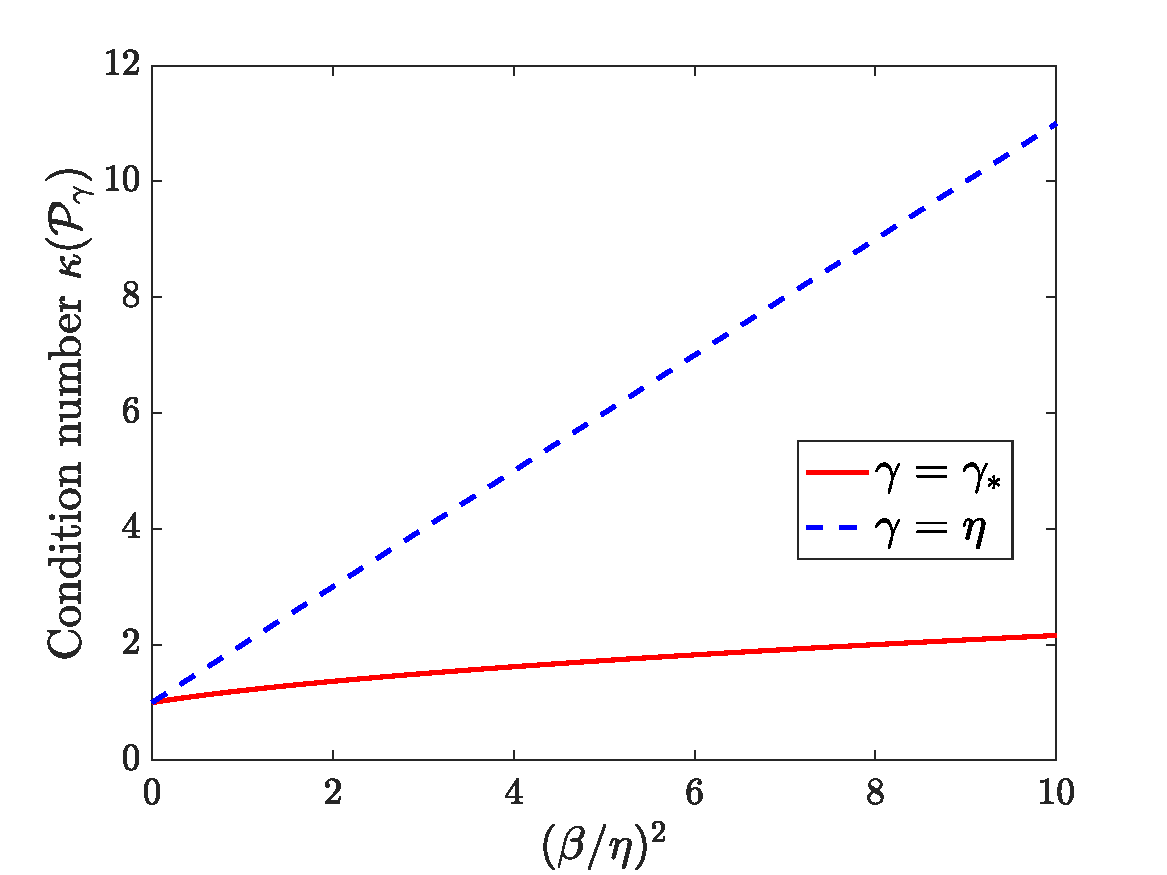
\includegraphics[width = 0.7\textwidth]{figures/conds_spsd}
\caption{Condition number of SPD ${\cal P}_{\gamma}$ for the optimal case of $\gamma = \gamma_*$ \eqref{eq:sd_kappa_Py*}, and non-optimal case of $\gamma = \eta$ \eqref{eq:sd_kappa_P_eta} as a function of $(\beta/\eta)^2$. }
\label{fig:conds}
\end{figure}

If using a simplified Newton algorithm, or solving a linear problem using this $2 \times 2$ formulation, one could likely save some work by setting $\gamma = \eta$ so that the preconditioner for the (1,1) block could also be used to precondition the Schur complement since \eqref{eq:sd_gamma*_and_kappa_gamma*} and \eqref{eq:sd_kappa_P_eta} are not too different for $\eta \gg \beta$.

\newpage
\tcb{An interesting exercise: Rather than $\gamma I - {\cal L}$, should the preconditioner instead look like $\widehat{S} = \gamma I - \zeta {\cal L}?$ To motivate this, look at the Schur complement, and assume that $\Vert 1/\eta {\cal L} \Vert < 1$,
\begin{align}
S = \eta I - {\cal L}  + \beta^2 (\eta I - {\cal L})^{-1} = \left( \eta + \frac{\beta^2}{\eta} \right) I - \left(1 - \frac{\beta^2}{\eta^2} \right) {\cal L} + {\cal O}\left( \frac{\beta^2}{\eta^3} {\cal L}^2 \right).
\end{align}
Does this say we should take the preconditioner to be
\begin{align}
\widehat{S} = \left( \eta + \frac{\beta^2}{\eta} \right) I - \left(1 - \frac{\beta^2}{\eta^2} \right) {\cal L}?
\end{align}
Quite interestingly, this gets $\gamma_* = \eta + \beta^2 / \eta$ correct. But what's weird is that for $\beta > \eta$, the sign of $\zeta$ changes from positive to negative. Nonetheless, the restriction of $\Vert 1/\eta {\cal L} \Vert < 1$ is not practical, even for an advection-dominated problem because it means imposing an explicit-like time step.
%
Actually, note that $\gamma I - \zeta {\cal L} = \zeta ( \gamma /\zeta I - {\cal L})$  has the same condition number as $\gamma/ \zeta  I - {\cal L}$ since they have the same spectrum upto scaling by $\zeta$. And, for this second matrix, we already showed the optimal constant in front of $I$ is $\gamma / \zeta = \eta + \beta^2 / \eta$, so if we choose $\gamma = \eta + \beta^2 / \eta$, then we should choose $\zeta = 1$.
}

\newpage
% ---------------------------------------------------------------------------------------------- %
% ---------------------------------------------------------------------------------------------- %
\subsection{The SPD case: Differing diagonal blocks}

As in later sections, here we consider a preconditioner of the form
\begin{align}
\widehat{S} = \gamma I -  {\cal L}_2,
\end{align}
for Schur complement
\begin{align}
S
= 
\left[ \eta I - {\cal L}_2 + \beta^2(\eta I - {\cal L}_1)^{-1} \right].
\end{align}
This results in a preconditioned operator
\begin{align}
{\cal P}
= 
S \widehat{S}^{-1} 
&= 
\left[ \eta I - {\cal L}_2 + \beta^2(\eta I - {\cal L}_1)^{-1} \right] 
\big[ \gamma I -  {\cal L}_2 \big]^{-1}, \\
&=
\big( \eta I - {\cal L}_2 \big) \big( \gamma I -  {\cal L}_2 \big)^{-1}  + \beta^2(\eta I - {\cal L}_1)^{-1} \big( \gamma I -  {\cal L}_2 \big)^{-1}.
\end{align}
Assuming that ${\cal L}_1$ and ${\cal L}_2$ are symmetric, and that they commute, ${\cal L}_1 {\cal L}_2 = {\cal L}_2 {\cal L}_1$, the preconditioned operator ${\cal P}$ is also symmetric by noting that if $AB = BA$, as is the case for $A = a I - {\cal L}_1$, $B = b I - {\cal L}_2$, then $A^{-1} B = B  A^{-1}$ and $A^{-1} B^{-1} = B^{-1} A^{-1}$.

Let $\lambda_1 \in \sigma(- {\cal L}_1) \subset [0,\infty)$ and $\lambda_2 \in \sigma(- {\cal L}_2) \subset [0,\infty)$. Denoting the spectrum of ${\cal P}$ by ${\cal F}$, we have
\begin{align}
{\cal F} 
= 
1 - 
\frac{\gamma - \eta}{\gamma + \lambda_2}
+
\frac{\beta^2}{(\eta + \lambda_1)(\gamma + \lambda_2)}.
\end{align}
Note that ${\cal F} > 0$ if $\gamma > 0$, i.e., ${\cal P}$ is SPD for $\gamma > 0$.

Differentiating ${\cal F}$ w.r.t. $\lambda_1$ and $\lambda_2$ we have
\begin{align}
{\cal F}_{\lambda_1} = -  \frac{\beta^2}{(\eta + \lambda_1)^2(\gamma + \lambda_2)}, 
\quad
{\cal F}_{\lambda_1} =  \frac{(\gamma-\eta)(\eta + \lambda_1) - \beta^2}{(\eta + \lambda_1)(\gamma + \lambda_2)}.
\end{align}
Clearly ${\cal F}_{\lambda_1} < 0$, while ${\cal F}_{\lambda_2} = 0$ for $\lambda_1^* = \frac{\beta^2}{\gamma - \eta} - \eta$. However, we also observe that ${\cal F}_{\lambda_2 \lambda_2}$ vanishes at  $\lambda_1^*$, so this is a point of inflection rather than a minimum or maximum, which is what we care  about. Thus, the extrema of ${\cal F}$ must occur at the boundaries of its domain. \tcb{This is fundamentally different to what occurred previously when the diagonal blocks were identical: The minimum of ${\cal F}$ occurred at a critical point in the eigenvalue $\lambda$.}

Basically, we find the following for ${\cal F}(\lambda_1, \lambda_2)$:
\begin{align}
{\cal F}(0,0) = \frac{1}{\gamma} \left( \eta + \frac{\beta^2}{\eta} \right), 
\quad 
{\cal F}(\infty, 0) = \frac{\eta}{\gamma},
\quad 
{\cal F}(0, \infty) = {\cal F}(\infty, \infty) = 1.
\end{align}
Assuming the spectra of  ${\cal L}_1$ and ${\cal L}_2$ are dense in $[0, \infty)$, this leads to the condition number
\begin{align}
\textrm{cond} ({\cal P}) = 
\begin{cases}
\displaystyle
\frac{1}{\gamma} \left( \eta + \frac{\beta^2}{\eta} \right), \quad &0 < \gamma \leq \eta, \\
\displaystyle
1 + \frac{\beta^2}{\eta^2}, \quad &\eta \leq \gamma \leq \eta + \frac{\beta^2}{\eta}, \\
\displaystyle
\frac{\gamma}{\eta}, \quad &\eta + \frac{\beta^2}{\eta} \leq \gamma < \infty.
\end{cases}
\end{align}
This condition number is minimized for \underline{\textbf{the entire inverval}} $\gamma \in \gamma_*  \coloneqq [\eta, \eta + \frac{\beta^2}{\eta}]$, in which case the minimum condition number is
\begin{align}
\textrm{cond} ({\cal P}_{\gamma \in \gamma_*}) = 1 + \frac{\beta^2}{\eta^2}.
\end{align}
A few remarks are in order:
\begin{itemize}
\setlength\itemsep{2ex}
 
\item Very weird how there is no longer an optimal value of $\gamma$, but instead a continuous interval of them. 

\item This condition number is dissapointingly large compared to the one in \eqref{eq:cond_min} that we get when ${\cal L}_1 = {\cal L}_2$. I think this is saying something about $\gamma I - {\cal L}_2$ not being a very good preconditioner... Since this grows too quickly w.r.t. $\beta$, I think it says that we're not doing a good enough job on the $\beta^2 (\eta I - {\cal L}_1)^{-1}$ that appears in the Schur complement. See the analysis I started in the next section to try and overcome this, but I'm not really sure it's any better/even makes sense.
  
\item Note that the analysis in here works out much the same as for the ${\cal L}_1 = {\cal L}_2$ case, except for the fact that the minimum of ${\cal F}$ does not occur at a critical point in $\lambda$, but instead at the boundary.
 
\item I somehow would have expected to recover the previous result in the case  that ${\cal L}_1 = {\cal L}_2$... But I guess the reason that this didn't happen is because when we differentiated, we assumed that $\lambda_1$ and $\lambda_2$ are independent, where, to actually recover the previous result, we'd have to assume they're the same. Is there any reason to assume that $\lambda_1$ and $\lambda_2$ would be related if ${\cal L}_1$ and ${\cal L}_2$ commute?
 
\item This result is consistent with the general analysis that arrived at bound \eqref{eq:gammastar}. It also explains why that bound is so much larger than in the case that ${\cal L}_1 \neq {\cal L}_2$: I.e., the preconditioner for ${\cal L}_1 \neq {\cal L}_2$ is simply not as good, as we've shown here for the SPD case.
 
\end{itemize}


\newpage
% ---------------------------------------------------------------------------------------------- %
% ---------------------------------------------------------------------------------------------- %
\subsection{The SPD case: Differing diagonal blocks with a modified preconditioner}

As we saw in the previous section, the preconditioner $\widehat{S} = \gamma I - {\cal L}_2$ doesn't produce great results in the sense that the condition number of the preconditioned operator grows quadratically in $\beta/\eta$. Notice in the Schur complement, the $\beta$ term weights a term containing an ${\cal L}_1$, but not a ${\cal L}_2$ term. Given that the condition number of the preconditioner grows too quickly with $\beta$, this possibly suggests that we try a preconditioner which also includes some ${\cal L}_1$ dependence. \tcb{I guess this follows on kind of from the discussion at the end of the SPD case with ${\cal L}_1 = {\cal L}_2$, where we see that modifying the ${\cal L}$ perturbation in the preconditioner influences the $\beta^2$ term. E.g., you can do the same Taylor series trick here for the Schur complement where ${\cal L}_1 \neq {\cal L}_2$.}

Let's again assume that ${\cal L}_1 {\cal L}_2 = {\cal L}_2 {\cal L}_1$, but let's say now we try a preconditioner of the form
\begin{align}
\widehat{S} = \gamma I - (\alpha {\cal L}_1 + (1 - \alpha) {\cal L}_2),
\end{align}
where the coefficients must sum to one for consistency with the case that ${\cal L}_1 = {\cal L}_2$ [although, I'm not sure this is necessary, actually...]. The preconditioned operator takes the form
\begin{align}
{\cal P}
= 
S \widehat{S}^{-1} 
= 
\left[ \eta I - {\cal L}_2 + \beta^2(\eta I - {\cal L}_1)^{-1} \right] 
\big[ \gamma I - (\alpha {\cal L}_1 + (1 - \alpha) {\cal L}_2) \big]^{-1}.
\end{align}
Let $\lambda_1 \in \sigma(- {\cal L}_1)$ and $\lambda_2 \in \sigma(- {\cal L}_2)$. Denoting the spectrum of ${\cal P}$ by ${\cal F}$, we have
\begin{align*}
{\cal F} 
&= \frac{\eta + \lambda_2}{\gamma + \alpha \lambda_1 + (1-\alpha) \lambda_2} + \frac{\beta^2}{(\eta + \lambda_1)(\gamma + \alpha \lambda_1 + (1-\alpha) \lambda_2)}, \\
\end{align*}
We can put some conditions on $\alpha$ as follows. We require ${\cal F} > 0$ to maintain positive definiteness. Noting that the numerators of each fraction are non-negative, and assuming $\gamma > 0$, this means
\begin{align*}
\gamma + \alpha \lambda_1 + (1 - \alpha) \lambda_2 > 0 
\quad \Longrightarrow \quad 
\alpha > - \frac{\lambda_2 + \gamma}{\lambda_1 - \lambda_2} < 0
\quad \textrm{and} \quad 
\alpha < \frac{\lambda_2 + \gamma}{\lambda_2 - \lambda_1} < 1.
\end{align*}
Thus, $\quad 0 \leq \alpha < 1$.
%
Also, we require that the first fraction in ${\cal F}$ remains bounded w.r.t. $\lambda_2$. We have
\begin{align*}
\lim \limits_{\lambda_2 \to \infty} \frac{\eta + \lambda_2}{\gamma + \alpha \lambda_1 + (1-\alpha) \lambda_2} 
&= 
\lim \limits_{\lambda_2 \to \infty} \frac{\tfrac{\eta}{\lambda_2} + 1}{\tfrac{\gamma}{\lambda_2} + \alpha \tfrac{\lambda_1}{\lambda_2} + (1-\alpha) } 
=
\lim \limits_{\lambda_2 \to \infty}
\frac{1}{1 - \alpha + \alpha \tfrac{\lambda_1}{\lambda_2}}.
\end{align*}
Noting that $\lambda_1$ and $\lambda_2$ are independent, this fraction remaining bounded and positive once again requires $0 \leq \alpha < 1$. Note that for $\alpha = 0$ we recover the previous preconditioner, $\gamma I - {\cal L}_2$.

Computing critical points is painful... Also, not quite sure how to compute ${\cal F}$ as $\lambda_1, \lambda_2 \to \infty$ due to them appearing together in first fraction...




\newpage
% ---------------------------------------------------------------------------------------------- %
% ---------------------------------------------------------------------------------------------- %
\section{Eigenvalue analysis of the skew symmetric case}
Assume ${\cal L}^\top = - {\cal L}$, as for central-finite-difference discretizations of a constant-coefficient advection problem, for example. While ${\cal L}$ is not going to be skew symmetric for a \textit{real-world problem}, it is a useful case to analyze because a \textit{good} advection discretization will have eigenvalues with large imaginary components, and skew symmetric matrices have purely imaginary eigenvalues; note that an \textit{exact} advection discretization would have purely imaginary eigenvalues. So while this case probably won't play out exactly in practice, I think it's a useful one to analyze and will hopefully provide some insight.

Some motivation here is that with the linear algorithm, which has a slightly different setup than this $2 \times 2$ problem, Ben observed a huge reduction in iteration count for an advection-dominated problem when using $\gamma = \gamma_*$ v.s. $\gamma = \eta$ compared with the typical types of reduction in iterations we see for diffusion-dominated problems. So, can we say anything about the optimal value $\gamma_*$, and/or whether $\gamma_*$ is significantly better than $\eta$ in this instance? Let's not set any restrictions of $\gamma$ yet, except that $\gamma \in \mathbb{R}$, so that we are left with a real matrix to invert. \tcr{Maybe it's worth redoing the following analysis for the linear case, because I'm not really sure the results I get here entirely correspond with what Ben observed numerically. Although, this difference could possibly have arisen because of an assumption I make on the size of the eigenvalues (see below), or maybe the skew-symmetric assumption I make is not a good one for the discretization/problem he tested.}

Let $\mathrm{i} \lambda \in \sigma(- {\cal L}) \subset [-\mathrm{i} c, \mathrm{i} c]$, for $\lambda \in \mathbb{R}$, $c \in \mathbb{R}_+$. For example, for a discretization of an advection problem with spacial mesh size $h$, we'd have $c \sim \delta t / h$. We're also going to assume that $\lambda$ is dense in $[-c,c]$, such that we can  treat it continuously. Note that doing so provides an upper bound on the condition number for finite-dimensional matrices who do not have such dense spectra.

The preconditioned operator is
\begin{align}
\label{eq:P_gamma_skew}
{\cal P}_{\gamma} 
= 
S \widehat{S}_{\gamma}^{-1} 
= 
\left[ \eta I - {\cal L} +  \beta^2 (\eta I - {\cal L})^{-1} \right] (\gamma I - {\cal L})^{-1}.
\end{align} 

\tcb{OK. Here's an afterthought which would have been useful to apply from the start. Notice how whenever we do these eigenvalue analyses we always end up with a condition number that doesn't depend on $\eta$ and $\beta$ independently, but only ever in the ratio $\beta/\eta$ (actually though, it seems to always depend on the square of this ratio)? This is because the preconditioned operator \eqref{eq:P_gamma_skew} actually only depends on them in this ratio. Observe that for $\beta \neq 0$,
\begin{align*}
{\cal P}_{\gamma} 
&= 
\tfrac{1}{\beta} \left[ \eta I - {\cal L} +  \beta^2 (\eta I - {\cal L})^{-1} \right] \beta (\gamma I - {\cal L})^{-1}, 
\\
&=
\left[ \tfrac{\eta}{\beta} I - \tfrac{1}{\beta} {\cal L} + (\tfrac{\eta}{\beta} I - \tfrac{1}{\beta} {\cal L})^{-1} \right] \left(\tfrac{\gamma}{\beta} I - \tfrac{1}{\beta} {\cal L} \right)^{-1},
\\
&=
\left[ x I - {\cal N} + (x I -  {\cal N})^{-1} \right] \left(y I - {\cal N} \right)^{-1} = {\cal P}_y,
\end{align*}
with $x = \eta \ /\beta > 0$, $y = \gamma / \beta > 0$ (assuming $\gamma > 0$), and ${\cal N} = {\cal L}/\beta$. So moving forward, we should be applying these transforms to simplify the analysis by reducing the parameter space by one dimension. We can see this symmetry in the original $2 \times 2$ system \eqref{eq:block} if we multiply each of the rows by $1/\beta$, which is why the Schur complement above ends up with the structure of $A + A^{-1}$.}

Assuming ${\cal L}$ is diagonalizable, the spectrum ${\cal F}_{\gamma}$ of ${\cal P}_{\gamma}$ is given by
\begin{align}
\label{eq:F_skew}
{\cal F}_{\gamma}(\lambda) = \frac{(\eta + \mathrm{i} \lambda)^2 + \beta^2}{(\gamma + \mathrm{i} \lambda) (\eta + \mathrm{i} \lambda)}.
\end{align}
Since ${\cal L}$ is normal, ${\cal P}_{\gamma}$ is too, and, thus, has a condition number
\begin{align*}
\kappa ({\cal P}_{\gamma}) = \frac{\max \limits_{\lambda \in [-c, c]}  |{\cal F}_{\gamma}(\lambda)|}{\min \limits_{\lambda \in [-c, c]}  |{\cal F}_{\gamma}(\lambda)|}.
\end{align*}
To analyze the extrema of $|{\cal F}_{\gamma}|$ we work with its square since it's easier,
\begin{align} 
\label{eq:G_def}
{\cal G}_{\gamma}(\lambda) 
\coloneqq
|{\cal F}_{\gamma}(\lambda)|^2 
=
{\cal F}_{\gamma}^{*}(\lambda) {\cal F}_{\gamma}(\lambda)
&=
\frac{\lambda^4 +  2(\eta^2 - \beta^2) \lambda^2 + (\eta^2 + \beta^2)^2}{\lambda^4 + (\eta^2 + \gamma^2) \lambda^2 + \eta^2 \gamma^2}, \\
&=
\frac{\lambda^4 +  2(\eta^2 - \beta^2) \lambda^2 + (\eta^2 + \beta^2)^2}{(\lambda^2 + \eta^2)(\lambda^2 + \gamma^2)} > 0,
\end{align}
where
\begin{align}
\label{eq:cond_skew_def}
\kappa^2 ({\cal P}_{\gamma}) = \frac{\max \limits_{\lambda \in [-c, c]}  {\cal G}_{\gamma}(\lambda)}{\min \limits_{\lambda \in [-c, c]}  {\cal G}_{\gamma}(\lambda)}.
\end{align}


\begin{itemize}
\setlength\itemsep{1ex}

\item I'm just going to \underline{assume $\beta > 0$} because it's too complicated to allow for all the edge cases if I don't. Anyway, it's obvious from \eqref{eq:P_gamma_skew} that the optimal choice if $\beta = 0$ is $\gamma = \eta$ since we get ${\cal P}_{\gamma} = I$.

\item For simplicity, let's just consider $c \to \infty$. While this won't arise in practice (where $c \sim \delta t / h$), it's helpful from an analysis point of view, since determining whether ${\cal G}_{\gamma}$ for some arbitrary $c < \infty$ is an extremum will be too complicated. However, note that considering $c \to \infty$ results in an upper bound on the condition number for finite $c$, since the min/max of $|{\cal F}|$ for $\lambda \in [-c,c]$ are bounded below/above by those in $(-\infty, \infty)$. Also, I think letting $c \to \infty$ is not such a bad assumption for big time steps, like $\delta t \sim 10 \delta x$. \tcr{Maybe come back and think some more about the case of finite $c$, I have some thoughts.}

\item Observe that as $\lambda \to \pm \infty$, ${\cal G}_{\gamma}$ approaches unity:
\begin{align}
\label{eq:Gunity}
\lim \limits_{\lambda \to \pm \infty} {\cal G}_{\gamma}(\lambda) 
= 
\frac{1 + 2(\eta^2 - \beta^2)\tfrac{1}{\lambda^2} + (\eta^2 + \beta^2)^2\tfrac{1}{\lambda^4}}{1 + (\eta^2 + \gamma^2)\tfrac{1}{\lambda^2} + \eta^2 \gamma^2 \tfrac{1}{\lambda^4}} 
=
\begin{cases}
1^{+}, \quad &\gamma^2 \leq \eta^2 - 2 \beta^2, \\
1^{-}, \quad &\gamma^2 > \eta^2 - 2 \beta^2.
\end{cases}
\end{align}
Based on this result, and the implications it has for the forthcoming analysis, we're going to \underline{assume} that 
\begin{align} 
\label{eq:gam_ass}
\gamma^2 > \eta^2 - 2 \beta^2, 
\quad
\textrm{and}
\quad
\gamma > \sqrt{\max(0, \eta^2 - 2 \beta^2)}.
\end{align}
Moreover, we're really only interested in the case where $\beta$ is at least of the order of $\eta$, which will allow us to take $\gamma$ down to zero. As such, I don't believe it's worth analyzing the other case.
Note we include the $\max$ here with 0 so that $\gamma^2  > 0$ since $\gamma \in \mathbb{R}_+$.

\item ${\cal G}_{\gamma}(\lambda)$ in \eqref{eq:G_def} is symmetric about $\lambda  = 0$, thus:
\begin{enumerate}
\setlength \itemsep{1ex}

\item We need only analyze $\lambda \in [0, \infty)$ since the extrema are also symmetric

\item \underline{$\lambda = 0$ is a turning point} since ${\cal G}_{\gamma}$ is not constant and is symmetric about $\lambda = 0$. For reference, the value of ${\cal G}_{\gamma}(0)$ is
\begin{align} \label{eq:G0}
{\cal G}_{\gamma}(0) = \left[ \frac{1}{\gamma} \left( \eta +  \frac{\beta^2}{\eta} \right) \right]^2.
\end{align}
Notice that
\begin{align}
\label{eq:G0_sizes}
{\cal G}_{\gamma}(0) 
=
\begin{cases}
> 1, \quad &0 < \gamma <  \eta +  \frac{\beta^2}{\eta}, \\
1, \quad &\gamma =  \eta +  \frac{\beta^2}{\eta}, \\
< 1, \quad  &\eta +  \frac{\beta^2}{\eta} < \gamma < \infty.
\end{cases}
\end{align}
\end{enumerate}


\item \underline{What kind of turning point is $\lambda = 0$?} To consider this, apply a Taylor series expansion about $\lambda = 0$ to get
\begin{align}
\label{eq:G_taylor}
{\cal G}_{\gamma}(\lambda) 
= 
{\cal G}_{\gamma}(0) 
+
\frac{1}{(\eta \gamma)^4} 
\Big[ 
\big( \eta^4 - 4 \eta^2 \beta^2 - \beta^4 \big) \gamma^2  - \eta^2 (\eta^2 + \beta^2)^2 
\Big] \lambda^2
+ 
{\cal O}(\lambda^4)
\end{align}
If the ${\cal O}(\lambda^2)$ term is positive, $\lambda = 0$ is a local minimum since we approach ${\cal G}_{\gamma}(0)$ from above. Conversely, if this term is negative, $\lambda = 0$ is a local maximum since we approach ${\cal G}_{\gamma}(0)$ from below. This can be restated as
\begin{align}
\Big[ \big(\eta^2 + \big(\sqrt{5}-2 \big) \beta^2 \big) \big(\eta^2 - \big( \sqrt{5}+2 \big) \beta^2 \big) \Big] \gamma^2 < \eta^2 (\eta^2 + \beta^2)^2
\quad 
\Longleftrightarrow 
\quad
\lambda = 0 \textrm{ is a local maximum!}
\end{align}
Notice that the first factor on the left-hand side is always positive, so if $\eta^2 \leq \big(\sqrt{5}+2 \big) \beta^2$, the left-hand-side is non positive, and the inequality is trivially true since the right-hand-side is positive. On the other hand, if $\eta^2 > \big(\sqrt{5}+2 \big) \beta^2$, then for $\lambda = 0$ to be a local maximum requires
\begin{align}
\label{eq:Kdef}
\gamma < \frac{\eta (\eta^2 + \beta^2)}{\sqrt{\eta^4 - 4 \eta^2 \beta^2 - \beta^4}} \eqqcolon {\cal K}. 
\end{align}
So, more concisely, we have the result
\begin{equation}
\label{eq:G0_class}
\begin{aligned}
\eta^2 \leq \big(\sqrt{5}+2 \big) \beta^2:& 
\quad 
{\cal G}_{\gamma}(0) = \textrm{local maximum}, \\
\eta^2 > \big(\sqrt{5}+2 \big) \beta^2:&
\quad
{\cal G}_{\gamma}(0) = 
\begin{cases}
\textrm{local maximum}, \quad  0 < \gamma < {\cal K}, \\
\textrm{local minimum}, \quad  {\cal K} <  \gamma  < \infty.
\end{cases}
\end{aligned}
\end{equation}

Noting that $\eta^4 > \eta^4 - 4 \eta^2 \beta^2 - \beta^4$, a sufficient condition that $\lambda = 0$ is always a local maximum is thus
\begin{align} \label{eq:suff_0max}
\gamma \leq \eta + \frac{\beta^2}{\eta} < {\cal K}.
\end{align}
Since ${\cal K} > \eta + \beta^2 / \eta$, ${\cal G}_{\gamma}(0) < 1$ when it is a local minimum due to \eqref{eq:G0_sizes}.

\item Taking the derivative of ${\cal G}$ in \eqref{eq:G_def}, we have
\begin{align} \label{eq:G_partial_skew}
\frac{\partial {\cal G}_{\gamma}}{\partial \lambda} 
= 
-\lambda
\frac{
(-\eta^2 + 2 \beta^2 + \gamma^2)\lambda^4 
- \big[ 2(\beta^2 + \eta^2)^2 - 2 \eta^2 \gamma^2  \big] \lambda^2 
+ \big[ \big( \eta^4 - 4 \eta^2 \beta^2 - \beta^4 \big) \gamma^2  - \eta^2 (\eta^2 + \beta^2)^2 \big] }
{(\gamma^2 + \lambda^2)^2 (\eta^2 + \lambda^2)^2}.
\end{align}
We immediately see the critical point $\lambda = 0$ that we just discussed. 
%
The denominator of \eqref{eq:G_partial_skew} is always positive, and, so, critical points of ${\cal G}$ occur at roots of the numerator, which we note is a quadratic function in the variable $\zeta \coloneqq \lambda^2 \geq 0$. We write this quadratic equation as
\begin{align}
\label{eq:Q_def_skew}
Q(\zeta) = a \zeta^2 + b \zeta + c,
\end{align}
with coefficients
\begin{equation}
\begin{gathered}
\label{eq:abc_def}
a \coloneqq -\eta^2 + 2 \beta^2 + \gamma^2, 
\quad
b \coloneqq - \big[ 2(\eta^2 + \beta^2)^2 - 2 \eta^2 \gamma^2  \big], \\
c \coloneqq \big( \eta^4 - 4 \eta^2 \beta^2 - \beta^4 \big) \gamma^2  - \eta^2 (\eta^2 + \beta^2)^2.
\end{gathered}
\end{equation}
Thus, the four remaining (other than $\lambda = 0$) possible critical points of ${\cal G}_{\gamma}$ occur at $\lambda = \pm \sqrt{\zeta_{\pm}}$, where $\zeta_{\pm}$ satisfy $Q(\zeta_{\pm}) = 0$. Note, however, that critical points $\zeta_{-} < 0$ or $\zeta_+ < 0$ are not valid since they'd correspond to imaginary values of $\lambda$.

Due to assumption \eqref{eq:gam_ass} resulting in ${\cal G}_{\gamma}$ approaching 1 from below as $\lambda \to \infty$, when ${\cal G}_{\gamma}(0)$ is a local maximum only one of $\zeta_-$ and $\zeta_+$ can be a turning point, and it must be a local minimum; note that the other critical point is not necessarily invalid/non-existent, it could be a point of inflection. Similarly, when ${\cal G}_{\gamma}(0)$ is a local minimum, either both $\zeta_{\pm}$ are local extrema (one being a max and the other a min), or neither of them are local extrema, in which case one or both could be points of inflection.

Let's examine the signs of the coefficients \eqref{eq:abc_def}. Note $a > 0$ always by assumption \eqref{eq:ass1}. For the second coefficient, $b < 0$ for $\gamma < \eta + \beta^2 / \eta$, $b = 0$ for $\gamma = \eta + \beta^2 / \eta$, and $b > 0$ for $\gamma > \eta + \beta^2 / \eta$. Notice that $c$ appeared exactly in the Taylor expansion \eqref{eq:G_taylor}. Thus, there is a direct correspondence between the sign of $c$ and the nature of ${\cal G}_{\gamma}(0)$: If ${\cal G}_{\gamma}(0)$ is a local maximum $c < 0$, and conversely, if ${\cal G}(0)$ is a local minimum $c > 0$. \\

Now, the roots of $Q$ in \eqref{eq:Q_def_skew} may be expressed as
\begin{align} \label{eq:zeta_pm}
\zeta_{\pm} = \frac{-b \pm \sqrt{b^2 - 4ac}}{2a}, \quad a > 0.
\end{align}
Computing the discriminant of $Q$ we find
\begin{align*}
b^2 - 4ac = 4 \beta^2 (\beta^2 + 4 \eta^2) w(\gamma),
\end{align*}
where we've defined the axillary function $w$,
\begin{align}
\label{eq:w_def}
w(\gamma) 
&\coloneqq 
\gamma^4 - 2( \eta^2 - \beta^2) \gamma^2 + \left( \eta^2 + \beta^2 \right)^2 \\
\label{eq:w_pos}
&=
\beta^4 + (\gamma^2 - \eta^2)^2 + 2 \beta^2(\gamma^2 + \eta^2) > 0. 
\end{align}
Thus, the discriminant is of $Q$ always positive, implying its roots $\zeta_{\pm}$ are always real.

Now we examine the signs of these roots to understand the nature of the critical points. Recall that if critical points $\zeta_{\pm}  < 0$ then they're to be discarded since they correspond to imaginary $\lambda$, so we examine under which conditions this happens. 
\begin{enumerate}
\setlength{\itemsep}{2ex}

\item From \eqref{eq:zeta_pm}, $\zeta_- < 0$ for any $b > 0$, and for $b<0$, we'd require $c < 0$ to have $\zeta_- < 0$. Working this through, and noting that ${\cal G}_{\gamma}(0)$ is never a local minimum for $\gamma < \eta + \beta^2 / \eta$, as in \eqref{eq:G0_class} and \eqref{eq:suff_0max}, we find that $\zeta_- < 0$ always, and so it is never a critical point.

\item From \eqref{eq:zeta_pm}, $\zeta_+ > 0$ for any $b < 0$, and for $b > 0$, we'd require $c < 0$ to have $\zeta_+ > 0$. Working this through, we find $\zeta_+ > 0$ when ${\cal G}_{\gamma}(0)$ is a local maximum, and $\zeta_+ < 0$ when ${\cal G}_{\gamma}(0)$ is a local minimum. Thus, $\zeta_+$ is a local minimum when ${\cal G}_{\gamma}(0)$ is a local maximum. And $\zeta_+$ is not a critical point when ${\cal G}_{\gamma}(0)$ is a local minimum. Moreover, we know that when $\lambda = \sqrt{\zeta_+}$ is a local minimum of ${\cal  G}_{\gamma}$, ${\cal G}_{\gamma}(\sqrt{\zeta_+}) < 1$ due to ${\cal G}_{\gamma}$ approaching unity from below as $\lambda \to \infty$, as in \eqref{eq:ass1}, and ${\cal G}_{\gamma}(0)$ being the only other turning point.

\end{enumerate}


\item Combining the above discussions, we can express the extrema of ${\cal G}_{\gamma}$ as follows. The minimum of ${\cal G}_{\gamma}$ is
\begin{align}
\min \limits_{\lambda \in \mathbb{R}} {\cal G}_{\gamma}(\lambda)
=
\begin{cases}
{\cal G}_{\gamma}(0) < 1, \quad &\textrm{ if } {\cal G}(0) \textrm{ is a local minimum}, \\
{\cal G}_{\gamma}(\sqrt{\zeta_+}) < 1, &\quad \textrm{else}.
\end{cases}
\end{align}
%
The maximum of ${\cal G}$ is
\begin{align}
\max \limits_{\lambda \in \mathbb{R}} {\cal G}_{\gamma}(\lambda)
=
\begin{cases}
{\cal G}_{\gamma}(0) \geq 1, \quad & 0 < \gamma \leq \eta + \frac{\beta^2}{\eta}, \\
1, \quad & \eta + \frac{\beta^2}{\eta} \leq \gamma  < \infty.
\end{cases}
\end{align}

Noting that ${\cal G}_{\gamma}(0)$ is always a local maximum for $\gamma < {\cal K}$, as in \eqref{eq:Kdef}, we can express the square of the condition number, as defined in \eqref{eq:cond_skew_def}, as
\begin{align} \label{eq:cond_val_skew}
\kappa^2({\cal P}_{\gamma}) =
\begin{cases}
\displaystyle
\frac{{\cal G}_{\gamma}(0)}{{\cal G}_{\gamma}(\sqrt{\zeta_+})}, 
\quad \sqrt{\max(\eta^2 - 2 \beta^2, 0)} < \gamma \leq \eta + \frac{\beta^2}{\eta}, \\[2.5ex]
\displaystyle
\frac{1}{{\cal G}_{\gamma}(\sqrt{\zeta_+})}, \quad \eta + \frac{\beta^2}{\eta} \leq \gamma < {\cal K}, \\[2.5ex]
\begin{cases}
\displaystyle
\frac{1}{{\cal G}_{\gamma}(\sqrt{\zeta_+})}, \quad &\textrm{ if } {\cal G}_{\gamma}(0) \textrm{ is a local maximum}, \\[2.5ex]
\displaystyle
\frac{1}{{\cal G}_{\gamma}(0)}, \quad &\textrm{ if } {\cal G}_{\gamma}(0) \textrm{ is a local minimum}, \quad \\
\end{cases},
\quad {\cal K} \leq \gamma < \infty.
\end{cases}
\end{align}

I had mostly given up at this point because computing ${\cal G}_{\gamma}(\sqrt{\zeta_+})$ as a function of $\gamma$ is awful, and Mathematica's \texttt{Simplify} just gave me a big mess. But actually, using Mathematica's \texttt{FullSimplify} to evaluate $1/{\cal G}_{\gamma}(\sqrt{\zeta_+})$ we get something tractable! Funnily enough, told to fully simplify ${\cal G}_{\gamma}(\sqrt{\zeta_+})$, it does so by putting a removable singularity at $\gamma = \eta$, which is not very helpful...\\

Anyway, we find that ${\cal G}_{\gamma}(\sqrt{\zeta_+})$ has the relatively simple form,
\begin{align}
\label{eq:g_d_def}
{\cal G}_{\gamma}(\sqrt{\zeta_+}) 
=
\frac{8 \eta^2 \beta}{g_{\rm d}(\gamma)}, \quad
g_{\rm d}(\gamma) \coloneqq
\beta \big( 3 \eta^2 + \beta^2 + \gamma^2 \big)  +  \sqrt{4 \eta^2 + \beta^2} \sqrt{w(\gamma)},
\end{align}
where $w$ is given by \eqref{eq:w_def}. Now we have the main result!
\begin{theorem}
Condition number \eqref{eq:cond_val_skew} is minimized with respect to $\gamma$ for 
\begin{align} 
\label{eq:gamma_opt_skew}
\gamma_* \coloneqq \underset{\sqrt{\max(\eta^2 - 2 \beta^2, 0)} < \gamma < \infty}{\textrm{argmin}} \kappa({\cal P}_{\gamma}) = \eta + \frac{\beta^2}{\eta},
\end{align}
and its minimum value is
\begin{align}
\label{eq:cond_opt_skew}
\kappa({\cal P}_{\gamma_*}) =  1 + \frac{1}{2} \left( \frac{\beta}{\eta} \right)^2.
\end{align}
\end{theorem}
\begin{proof}

The outline of the proof is as follows: We will first establish that for $\gamma > \eta + \beta^2/\eta$ condition number \eqref{eq:cond_val_skew} is strictly increasing. Then we will establish that the condition number is strictly decreasing in the interval $\sqrt{\max(\eta^2 - 2 \beta^2, 0)} < \gamma < \eta + \beta^2 / \eta$. It will therefore follow that the minimum is achieved at the intersection of these two domains, as in \eqref{eq:gamma_opt_skew}. 
%

Again, for simplicity, we work with the square of the condition number rather than the function itself. We remark that the derivative of function and the derivative of its square have the same sign because the function is positive: $[\kappa^2(\gamma)]' = 2 \kappa \kappa'$ implies $\textrm{sign}([\kappa^2]') = \textrm{sign}(\kappa')$ because $\kappa > 0$. \\

\underline{Case 1: $\gamma > \eta + \beta^2/\eta$} \quad We first consider the case in which ${\cal G}_{\gamma}(0)$ is a local maximum, such that the condition number \eqref{eq:cond_val_skew} is simply $1/{\cal G}_{\gamma}(\sqrt{\zeta_+})$. Notice from \eqref{eq:g_d_def}, that the only dependence of $1/{\cal G}_{\gamma}(\sqrt{\zeta_+})$ on $\gamma$ occurs through the dependence of $g_{\rm d}(\gamma)$ on it, so we just analyze the behaviour of this function.

Setting the derivative of $g_{\rm d}$ to zero, and searching for critical points $\gamma$, we immediately identify $\gamma =  0$ as a critical point (which it must be  by symmetry of the function in $\pm \gamma$ anyway). Working through the algebra, we find that the remaining critical points must satisfy the following equation
\begin{align}
\beta \sqrt{w} = - \sqrt{4 \eta^2 + \beta^2} (-  \eta^2 + \beta^2 + \gamma^2).
\end{align}
Notice that the equation has no solution if $\gamma^2 > \eta^2 - \beta^2$ since the left-hand side is positive while the right-hand side is negative. Thus, we conclude that critical points of $g_{\rm}$, if they exist, must occur for $\gamma^2 < \eta^2 - \beta^2$. \\

Actually, I guess this is enough to conclude that $g_{\rm d}$ is strictly increasing for $\gamma > \eta + \beta^2/\eta$, because we know that $g_{\rm d} \to \infty$ as $\gamma \to \infty$, and we've shown that if the function has critical points they must occur for $\gamma^2 < \eta^2 - \beta^2$, but $(\eta + \beta^2/\eta)^2 >  \eta^2 > \eta^2 - \beta^2$, therefore there are no critical points for $\gamma > \eta + \beta^2/\eta$. The following section in blue shows that actually the function is increasing for $\gamma > \sqrt{\max(\eta^2 - 2 \beta^2,0)}$, which I was initially using in the proof to show that $\kappa^2$ is decreasing for $\gamma \in (\sqrt{\max(\eta^2 - 2 \beta^2,0)}, \eta + \beta^2/\eta)$, but no longer am.

\tcb{
Further working through the algebra, assuming that $\gamma^2 < \eta^2 - \beta^2$, we find that such roots must satisfy a quartic equation, which can be expressed in factored form as
\begin{align*}
(\gamma^2 - \eta) \left[\gamma^2 - (\eta^2 - 2 \beta^2) \right] = 0.
\end{align*}
which we see immediately has the following pairs of solutions
\begin{align*}
\gamma^2 = \eta, \quad \gamma^2 = \eta^2 - 2 \beta^2.
\end{align*}
The first pair of solutions $\gamma^2 = \eta$ can be discarded immediately since they violate the inequality $\gamma^2 < \eta^2 - \beta^2$. Moreover, notice that the second pair of solutions is only valid when $\eta^2 - 2 \beta^2 > 0$.
%
Thus, we are left with three possible critical points of $g_{\rm d}$, $\gamma \in  \{0, \pm \sqrt{\eta^2 - 2 \beta^2} \}$. To classify these critical points, it is sufficient to examine the sign of $g_{\rm d}''(0)$ as follows. Computing this quantity, we find
\begin{align*}
g_{\rm d}''(0) = 2 \left( \beta - \sqrt{4 \eta^2 + \beta^2} \frac{ \eta^2 - \beta^2}{\eta^2 + \beta^2}  \right).
\end{align*}
If $g_{\rm d}''(0) > 0$, $\gamma = 0$ is a local minimum. If $g_{\rm d}''(0) < 0$, $\gamma =  0$ is a local maximum.
%
Working through, we find the following:
\begin{enumerate}
\setlength{\itemsep}{0.5ex}
\item $\gamma = 0$ is a local minimum if $\eta^2 - 2 \beta^2 < 0$
\item $\gamma = 0$ is a local maximum if $\eta^2 - 2 \beta^2 > 0$
\end{enumerate}
Remarking that $g_{\rm d}$ is unbounded as $\gamma \to \pm \infty$, and that the critical points $\gamma = \pm \sqrt{\eta^2 - 2 \beta^2}$ don't exist for $\eta^2 - 2 \beta^2 < 0$ allows us to classify the latter as local minima when they exist. Therefore, we can conclude the following:
\begin{align*}
g_{\rm d} \textrm{ is strictly increasing for } \gamma > \sqrt{\max(0, \eta^2 - 2 \beta^2)}.  
\end{align*}}

As such, when condition number \eqref{eq:cond_val_skew} is equal to $1/{\cal G}(\sqrt{\zeta_+}) \propto g_{\rm d}(\gamma)$ (see \eqref{eq:g_d_def}), is strictly increasing for $\gamma > \eta + \beta^2/\eta$. Consequently, the condition number does not achieve its minimum value in this interval, unless it occurs at the boundary, $\gamma = \eta + \beta^2/\eta$.\\

Now we briefly consider the case in which condition number \eqref{eq:cond_val_skew} is given by $1/{\cal G}_{\gamma}(0)$. As the critical point $\lambda = \sqrt{\zeta_+} \to 0^+$ of ${\cal G}_{\gamma}$, the local maximum at $\lambda = 0$ becomes a local minimum, and it is precisely this case in which condition number \eqref{eq:cond_val_skew} transitions from $1/{\cal G}_{\gamma}(\sqrt{\zeta_+})$ into $1/{\cal G}(0)$. Since $1/{\cal G}_{\gamma}(\sqrt{\zeta_+})$ and $1/{\cal G}_{\gamma}(0)$ are always decreasing for $\gamma > \eta + \beta^2/\eta$, it follows that ${\cal G}_{\gamma}(0)$ for $\gamma > {\cal K}$ is smaller than ${\cal G}_{\gamma}(\sqrt{\zeta_+})$ is for $\eta + \beta^2/\eta < \gamma < {\cal K}$. That is to say, when condition number \eqref{eq:cond_val_skew} is equal to $1/{\cal G}_{\gamma}(0)$, it is always larger than when it is equal to $1/{\cal G}_{\gamma}(\sqrt{\zeta_+})$.\\

\underline{Case 2: $\sqrt{\max(\eta^2 - 2 \beta^2, 0)} < \gamma < \eta + \beta^2/\eta$} \quad Having now established that $\kappa^2(\gamma)$ is strictly increasing for $\gamma > \eta + \beta^2/\eta$, we now show that it is strictly decreasing for $\gamma \in (\sqrt{\max(\eta^2 - 2 \beta^2, 0)}, \eta + \beta^2/\eta)$. Again, we work with the square of condition number \eqref{eq:cond_val_skew}, which in this interval can be expressed as
\begin{align}
\label{eq:cond_2}
\kappa^2(\gamma) = 
\frac{(\eta^2 + \beta^2)^2}{8 \eta^4 \beta} \frac{g_{\rm d}(\gamma)}{\gamma^2},
\quad
\gamma \in \left( \sqrt{\max(\eta^2 - 2 \beta^2, 0)}, \eta + \frac{\beta^2}{\eta} \right],
\end{align}
with $g_{\rm d}$ given in \eqref{eq:g_d_def}. The derivative is given by and can be bounded above as follows
\begin{align*}
[\kappa^2(\gamma)]' 
&= 
\frac{(\eta^2 + \beta^2)^2}{8 \eta^4 \beta} \frac{1}{\gamma^3} 
\big[  \gamma g_{\rm d}'(\gamma) - 2 g_{\rm d}(\gamma)
\big] \\
&=
\frac{(\eta^2 + \beta^2)^2}{4 \eta^4 \beta} \frac{1}{\sqrt{w} \gamma^3} 
\left[
\gamma^2
\big[\beta \sqrt{w} + \sqrt{4 \eta^2 + \beta^2} (-\eta^2 + \beta^2 + \gamma^2) \big] \right.\\ 
&  \left. 
\hspace{25ex} -\big[\beta(-\eta^2+\beta^2+\gamma^2) \sqrt{w} + \sqrt{4 \eta^2 + \beta^2} w \big] 
\right] \\
&=
\frac{(\eta^2 + \beta^2)^2}{4 \eta^4 \beta} \frac{1}{\sqrt{w} \gamma^3} 
\left[
-\beta(3 \eta^2 + \beta^2) \sqrt{w} + \big[ (\eta^2 - \beta^2) \gamma^2 -(\eta^2  + \beta^2) \big] \sqrt{4 \eta^2 + \beta^2} 
\right] \\
&<
\frac{(\eta^2 + \beta^2)^2}{4 \eta^4 \beta} \frac{\sqrt{4 \eta^2 + \beta^2} }{\sqrt{w} \gamma^3} 
\left[ (\eta^2 - \beta^2) \gamma^2 - (\eta^2  + \beta^2) \right].
\end{align*}
Now, we consider two cases individually. If $\eta \leq \beta$, the first term is clearly non-positive. Conversely, if $\eta > \beta$, then using that $\gamma \leq \eta + \beta^2/\eta$, we have 
\begin{align*}
(\eta^2 - \beta^2) \gamma^2 - (\eta^2 + \beta^2) \leq - \left[ \frac{\beta (\eta^2 + \beta^2)}{\eta} \right]^2 < 0.
\end{align*}
Applying both of the above results, we find $[\kappa^2]' < 0$ for $\gamma \leq \eta + \beta^2 / \eta$. \\

Finally, by virtue of its relationship with $\kappa^2$, $\kappa$ is strictly decreasing for $\sqrt{\max(\eta^2 - 2 \beta^2, 0)} < \gamma < \eta + \beta^2/\eta$, and strictly increasing for $\gamma > \eta + \beta^2/\eta$. Therefore $\kappa$ is minimized at the interface, $\gamma = \gamma_* = \eta + \beta^2/\eta$, as in \eqref{eq:gamma_opt_skew}. Evaluating \eqref{eq:cond_2} at $\gamma_*$ gives result \eqref{eq:cond_opt_skew}.\\
\end{proof}

\item

While $\kappa({\cal P}_{\gamma_*})$ in \eqref{eq:cond_opt_skew} is disappointingly large, it is only just smaller than the bound on it that Ben derived for general matrices ${\cal L}$, which was 
\begin{align} 
\label{eq:kappa_star_bound}
\kappa(\mathcal{P}_{\gamma_*}) \leq 2+\frac{\beta^2}{2\eta^2} - \frac{\beta^2}{2\eta^2+2\beta^2}
= 2 + \frac{1}{2} \left( \frac{\beta}{\eta} \right)^2 \frac{1}{(\eta/\beta)^2 + 1}
\end{align}
Notice that as $\beta/\eta \to \infty$, or $\eta/\beta \to 0$, this bound sits just slightly above $\kappa({\cal P}_{\gamma_*})$ for the SS case of \eqref{eq:cond_opt_skew}.

I guess this says that 1: That the bound Ben derived for general matrices is fairly tight because here we have a specific class of matrix for which it is tight. 2: Skew symmetric matrices lead to a fairly poorly conditioned ${\cal P}_{\gamma}$, in general, since we saw for SPSD matrices that the operator has a much smaller condition number.\\

Another case of interest is $\gamma = \eta$. Evaluating condition number \eqref{eq:cond_val_skew} for $\gamma = \eta$ we find
\begin{align}
\label{eq:kappa_eta_skew}
\kappa({\cal P}_{\eta}) = \frac{1}{2} \sqrt{4 + \left( \frac{\beta}{\eta} \right)^2} \left[ 1 + \left( \frac{\beta}{\eta} \right)^2 \right].
\end{align}
Clearly $\kappa({\cal P}_{\gamma_*}) < \kappa({\cal P}_{\eta})$. 

See Figure \ref{fig:conds_all} for a comparison of the condition numbers for the SS and SPSD cases, which also includes the general upper bound \eqref{eq:kappa_star_bound}.

\end{itemize}

\begin{figure}[!htb]
\label{fig:conds_all}
\centering
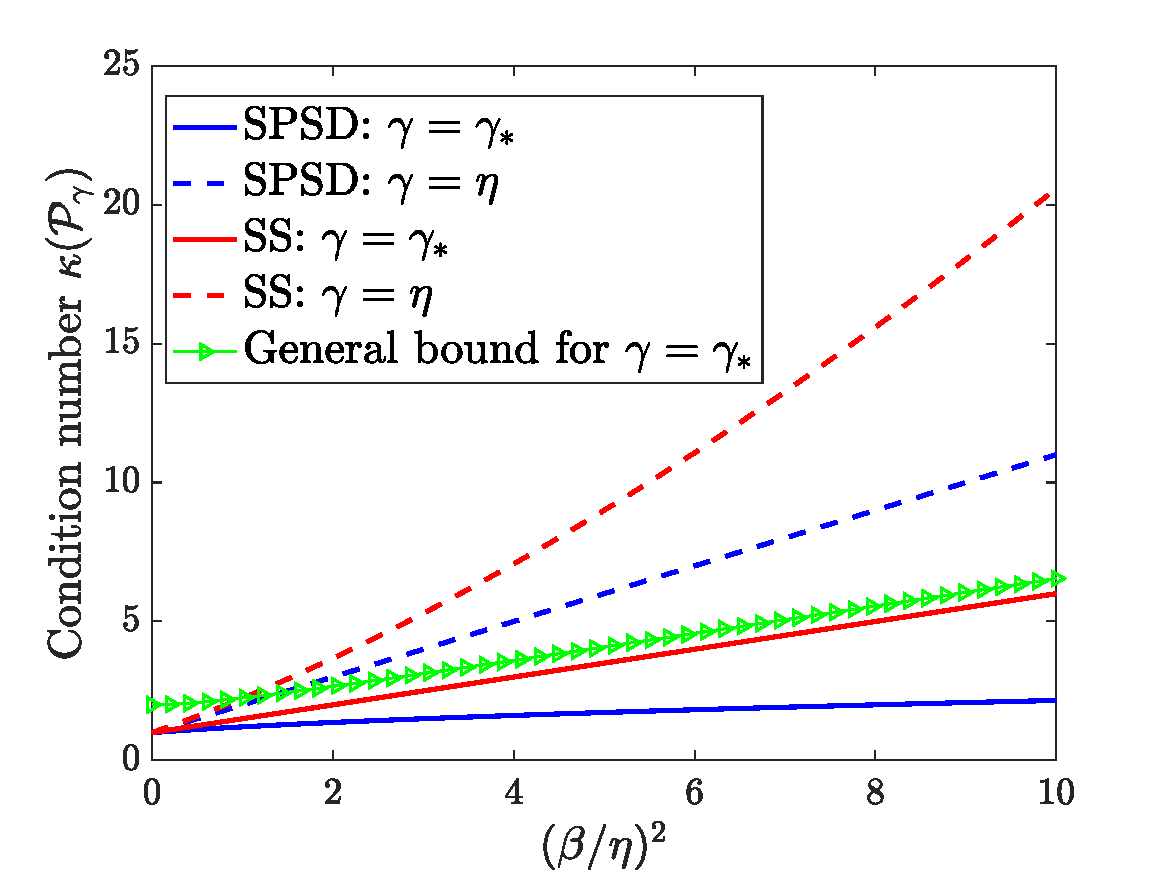
\includegraphics[width=0.65\textwidth]{figures/conds_spsd_ss}
\caption{Condition numbers of ${\cal P}_{\gamma}$ for SPSD and SS matrices ${\cal L}$ as a function of $(\beta/\eta)^2$. The SS condition numbers are \eqref{eq:cond_opt_skew} and \eqref{eq:kappa_eta_skew} for $\gamma = \gamma_*$ and $\gamma = \eta$, respectively. Also included is the general upper bound for the condition number of ${\cal P}_{\gamma_*}$ from \eqref{eq:kappa_star_bound}.}
\end{figure}

\subsection{Convergence of GMRES}

Convergence of GMRES applied to the $2 \times 2$ system is defined by convergence of GMRES on the preconditioned Schur complement, ${\cal P}_{\gamma}$ (at least I think that's how it works; pretty sure Ben has written that somewhere). So, given the above analysis, what can be said about the convergence of GMRES? \\

Assuming that the symmetric part of ${\cal P}_{\gamma}$, that is $\tfrac{1}{2}\left({\cal P}_{\gamma} +  {\cal P}_{\gamma}^\top \right)$, is positive definite, the $k$th GMRES residual may be bounded as
\begin{align} 
\label{eq:gmres_eig_bound}
\frac{\Vert \mathbf{r}_k \Vert_2}{\Vert \mathbf{r}_0 \Vert_2} \leq
\left[1 -  \frac{\mu_{\min}^2 \left( \tfrac{1}{2} \left( {\cal P}_{\gamma} +  {\cal P}_{\gamma}^\top \right) \right)}{\mu_{\max} \left( {\cal P}_{\gamma} {\cal P}_{\gamma}^\top \right)}  \right]^{k/2} \eqqcolon {\cal Z}_{\gamma}^{k/2},
\end{align}
where $\mu_{\min},\mu_{\max}$ represent  the minimum,maximum eigenvalues of the associated operator.

By the skew symmetry of ${\cal L}$, we have
\begin{align}
\label{eq:PT_gamma_skew}
{\cal P}_{\gamma}^\top = \left[ \eta I + {\cal L} +  \beta^2 (\eta I + {\cal L})^{-1} \right] (\gamma I + {\cal L})^{-1}.
\end{align}
So notice that ${\cal P}_{\gamma}^\top$ is the same as ${\cal P}_{\gamma}$, just with ${\cal L} \mapsto - {\cal L}$. As such, the spectrum of \eqref{eq:PT_gamma_skew} is simply ${\cal F}_{\gamma}(- \lambda)$, where ${\cal F}_{\gamma}(\lambda)$ is the spectrum of ${\cal P}_{\gamma}$ defined in \eqref{eq:F_skew}. Furthermore, the spectrum of ${\cal P}_{\gamma} {\cal P}_{\gamma}^\top $ is simply ${\cal F}_{\gamma}(- \lambda) {\cal F}_{\gamma}(\lambda) = {\cal F}_{\gamma}^*(\lambda) {\cal F}_{\gamma}(\lambda) = {\cal G}_{\gamma}(\lambda)$, as defined in \eqref{eq:G_def}.

So, we can immediately compute the maximum eigenvalue as follows
\begin{equation}
\begin{aligned}
\label{eq:mu_skew}
\mu_{\max} \left( {\cal P}_{\eta} {\cal P}_{\eta}^\top \right) 
&= {\cal G}_{\eta}(0)
= 
\left[ \left(\frac{\beta}{\eta}\right)^2 +1 \right]^2, 
\\
\mu_{\max} \left( {\cal P}_{\gamma_*} {\cal P}_{\gamma_*}^\top \right) 
&= {\cal G}_{\gamma_*}(0) 
= 
1,
\end{aligned}
\end{equation}
since we know that the max of ${\cal G}_{\gamma}$ is at $\lambda = 0$ for $\gamma \leq \eta + \beta^2 / \eta$. 

Letting
\begin{align*}
{\cal H}_{\gamma}(\lambda) \coloneqq \tfrac{1}{2} \left( {\cal F}_{\gamma}(- \lambda) + {\cal F}_{\gamma}(\lambda) \right)
\end{align*}
denote the spectrum of the symmetric part of ${\cal P}_{\gamma}$, we find
\begin{align*}
{\cal H}_{\eta}(\lambda) 
&= 
1 + \beta^2 \frac{(\eta - \lambda)(\eta + \lambda)}{(\eta^2 + \lambda^2)^2}
\\
{\cal H}_{\gamma_*}(\lambda) 
&= 
\eta^2 \frac{\beta^4 + 2 \eta^2 \beta^2 +  (\eta^2 + \lambda^2)^2}{(\eta^2 + \lambda^2) \left[ (\eta^2 + \beta^2)^2 + (\eta \lambda)^2 \right]}.
\end{align*}

For the global minima of these functions, we find
\begin{equation}
\begin{aligned}
\label{eq:H_min_skew}
\mu_{\min} \left( \tfrac{1}{2}  \left( {\cal P}_{\eta} +  {\cal P}_{\eta}^\top \right) \right) 
&= 
\underset{\lambda \in \mathbb{R}}{\min} \,  {\cal H}_{\eta}(\lambda) = 1 - \frac{1}{8} \left( \frac{\beta}{\eta} \right)^2, \\
\mu_{\min} \left( \tfrac{1}{2} \left( {\cal P}_{\gamma_*} +  {\cal P}_{\gamma_*}^\top \right) \right)
&=
\underset{\lambda \in \mathbb{R}}{\min} \,  {\cal H}_{\gamma_*}(\lambda) =  \frac{2}{\left( \beta/\eta \right)^2 + 2}. 
\end{aligned}
\end{equation}

\begin{remark}[Indefiniteness of symmetric part of ${\cal P}_{\eta}$]
Observe from \eqref{eq:H_min_skew} that the symmetric part of ${\cal P}_{\eta}$ is not always positive definite; for this to remain positive definite, it requires that $\beta / \eta < 2 \sqrt{2} \lesssim 2.83$. As such, bound \eqref{eq:gmres_eig_bound} cannot be applied for $(\beta / \eta)^2 > 8$, or $\beta / \eta \geq 2 \sqrt{2}$. Conversely, the symmetric part of ${\cal P}_{\gamma_*}$ is always positive definite since its minimum eigenvalue is positive (which we could see from the fact that the equation for ${\cal H}_{\gamma_*}(\lambda) $ above is always positive).
%
For reference, we also have
\begin{align*}
\underset{\lambda \in \mathbb{R}}{\max} \,  {\cal H}_{\eta}(\lambda) = 1 + \left( \frac{\beta}{\eta} \right)^2,
\quad
\underset{\lambda \in \mathbb{R}}{\max} \,  {\cal H}_{\gamma_*}(\lambda) = 1.
\end{align*}
So as $\left( \frac{\beta}{\eta} \right)^2$ increases and the symmetric component of ${\cal P}_{\eta}$ loses positive definitess, it become more and more indefinite since its maximum eigenvalue continues to increase also.   
%
This is interesting. Is there any significance other than GMRES bound \eqref{eq:gmres_eig_bound} cannot be applied? E.g., is it known that GMRES convergence for matrices with indefinite symmetric components is worse than those without? If something like this is true, then it definitely says that $\gamma = \eta$ is a poor choice for skew symmetric matrices. 
\end{remark}
I don't really know anything about GMRES convergence theory. But I did find the following From Corollary 3 of the GMRES paper by Saad and Schultz: ``\textit{...
A consequence of Proposition 2 is that the restarted algorithm GMRES(m) does
not break down. GMRES(m) would therefore constitute a very reliable algorithm if
it always converged. Unfortunately this is not always the case, i.e. there are instances
where the residual norms produced by the algorithm, although nonincreasing, do not
converge to zero. In [5] it was shown that the GCR (m-1) method converges under
the condition that A is positive real and so the same result is true for GMRES(m).
It is easy to construct a counter-example showing that this result does not extend to
indefinite problems, i.e. that the method may not converge if the symmetric part of A
is not positive definite. In fact it is possible to show that the restarted GMRES method
may be stationary.}'' 

So I guess from this, it probably is bad news for GMRES that for $\beta/\eta$ large enough the symmetric component of ${\cal P}_{\eta}$ becomes indefinite (since we're using restarted GMRES, that is).\\

Plugging the maxima and minima from \eqref{eq:mu_skew} and \eqref{eq:H_min_skew} into GMRES bound \eqref{eq:gmres_eig_bound} we find
\begin{align}
\label{eq:GMRES_bounds_skew}
{\cal Z}_{\eta} 
= 
\frac{9}{64} \left( \frac{\beta}{\eta} \right)^2 \frac{7 \left( \frac{\beta}{\eta} \right)^2 + 16}{\left[ \left( \frac{\beta}{\eta} \right)^2 + 1 \right]^2}, 
\quad 
\left( \frac{\beta}{\eta} \right)^2 < 8, 
\quad
{\cal Z}_{\gamma_*} = 1 - \frac{4}{\left[\left( \frac{\beta}{\eta} \right)^2 + 2 \right]^2}.
\end{align}



\begin{figure}[!htb]
\label{fig:gmres_bounds}
\centering
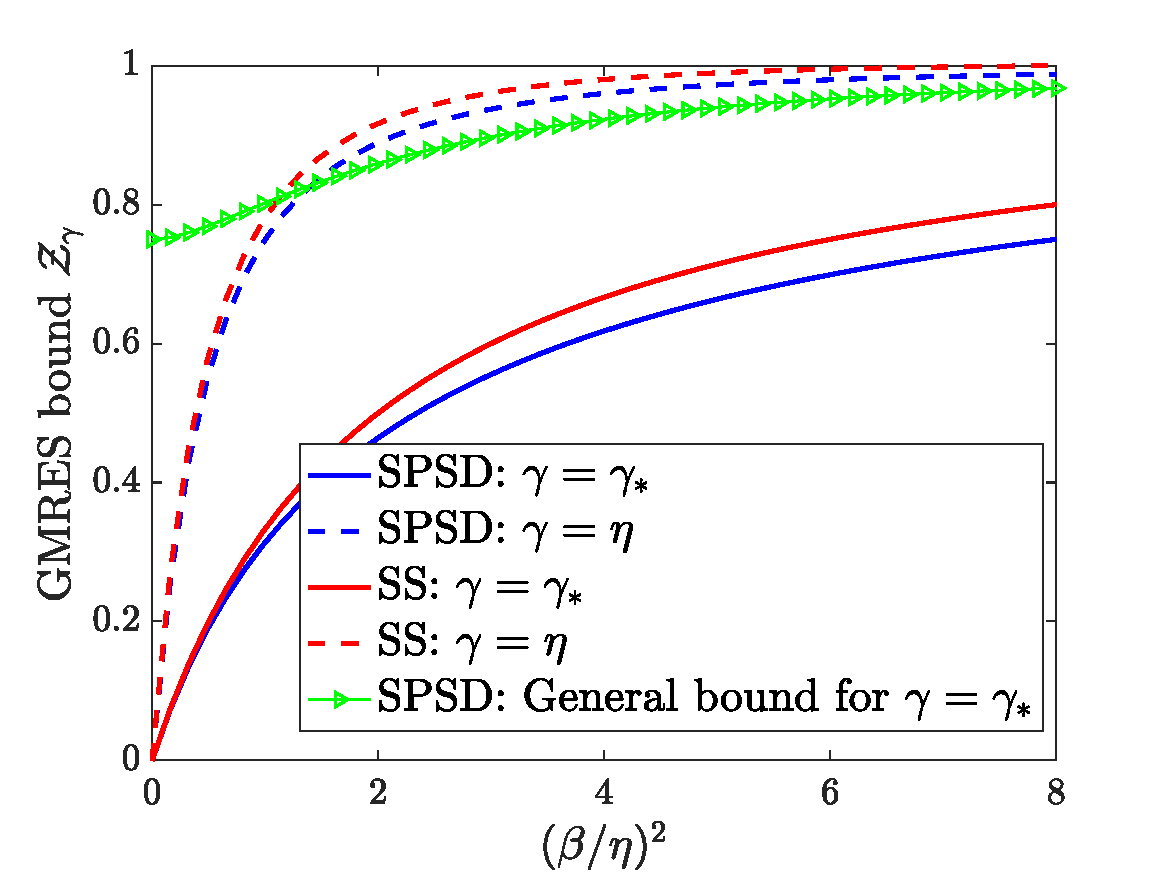
\includegraphics[width=0.65\textwidth]{figures/gmres_bounds_spsd_ss}
\caption{GMRES bound ${\cal Z}_{\gamma}$ from \eqref{eq:gmres_eig_bound} for SPSD and SS matrices ${\cal L}$ as a function of $(\beta/\eta)^2$. The SS bounds are given in \eqref{eq:GMRES_bounds_skew}. Also included is the GMRES bound for SPD ${\cal P}_{\gamma_*}$ that's calculated from upper bound on $\kappa({\cal P}_{\gamma_*})$ in \eqref{eq:kappa_star_bound}. Notice how the general GMRES bound for the SPSD case and the SS $\gamma_*$ cases asymptote towards each other; this regime also corresponds to when their condition numbers asymptote to each other, as discussed with \eqref{eq:kappa_star_bound}. I suppose this does demonstrates that condition number is a good proxy for how quickly GMRES will converge, even though bounds \eqref{eq:gmres_eig_bound} are more complicated than that for non SPD matrices. The SPD bounds are computed via their condition number with \eqref{eq:gmres_bounds_spd}.}.
\end{figure}

See Figure \ref{fig:gmres_bounds} for a plot of the GMRES bounds which also includes the SPSD convergence bounds. In the case of SPD ${\cal P}_{\gamma}$, bound \eqref{eq:gmres_eig_bound} can be computed in terms of condition number as 
\begin{align}
\label{eq:gmres_bounds_spd}
{\cal Z}_{\gamma} = 1 - \frac{1}{\kappa^2({\cal P}_{\gamma})} = \frac{\kappa^2({\cal P}_{\gamma}) - 1}{\kappa^2({\cal P}_{\gamma})}.
\end{align}


So the thing I was hoping to get out of this analysis was that for skew symmetric matrices, it was much more important that we use $\gamma_*$ v.s. $\eta$ than it is for SPSD problems. Recalling that in the linear algorithm, for a hyperbolic example, Ben saw a much larger reduction in iteration count when using $\gamma_*$ v.s. $\eta$ for a hyperbolic problem over a diffusive one. However, the plots in Figure \ref{fig:gmres_bounds} don't strongly suggest this is the case, but it is a little hard to tell because this is a convergence factor and has an inverse logarithmic relationship with the number of iterations. \\

To investigate further, let's assume that \eqref{eq:gmres_eig_bound} is relatively tight, and say we solve to a relative tolerance of $10^{-\varepsilon}$, then we can approximate the number of GMRES iterations $k$ as
\begin{align}
\label{eq:gmres_approx_iters}
10^{-\varepsilon} \approx {\cal Z}^{k/2} 
\quad \Longrightarrow \quad
k \approx \frac{-2 \varepsilon}{\log_{10} ({\cal Z}_{\gamma})}.
\end{align}

\begin{figure}[!htb]
\label{fig:gmres_iters}
\centering
\makebox[\textwidth][c]{
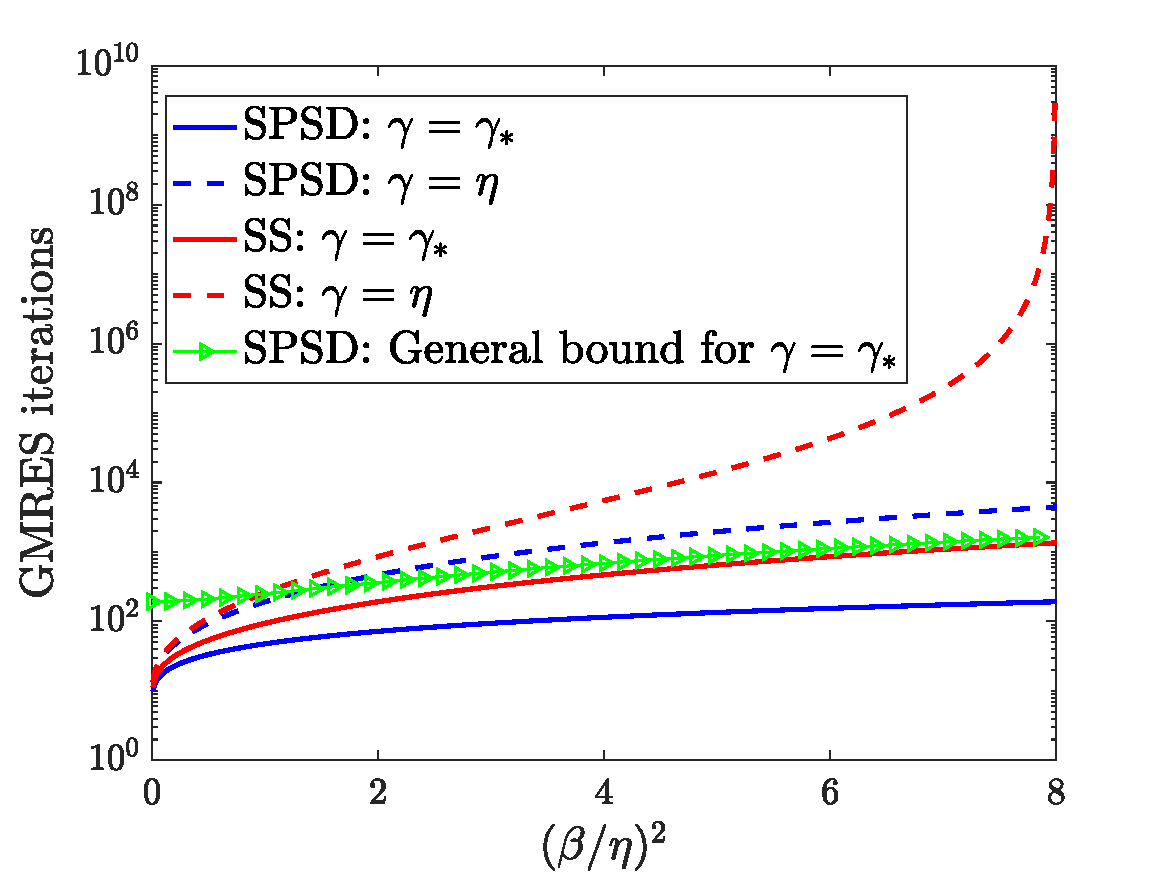
\includegraphics[width=0.575\textwidth]{figures/gmres_iters_spsd_ss}
\hspace{-5ex}
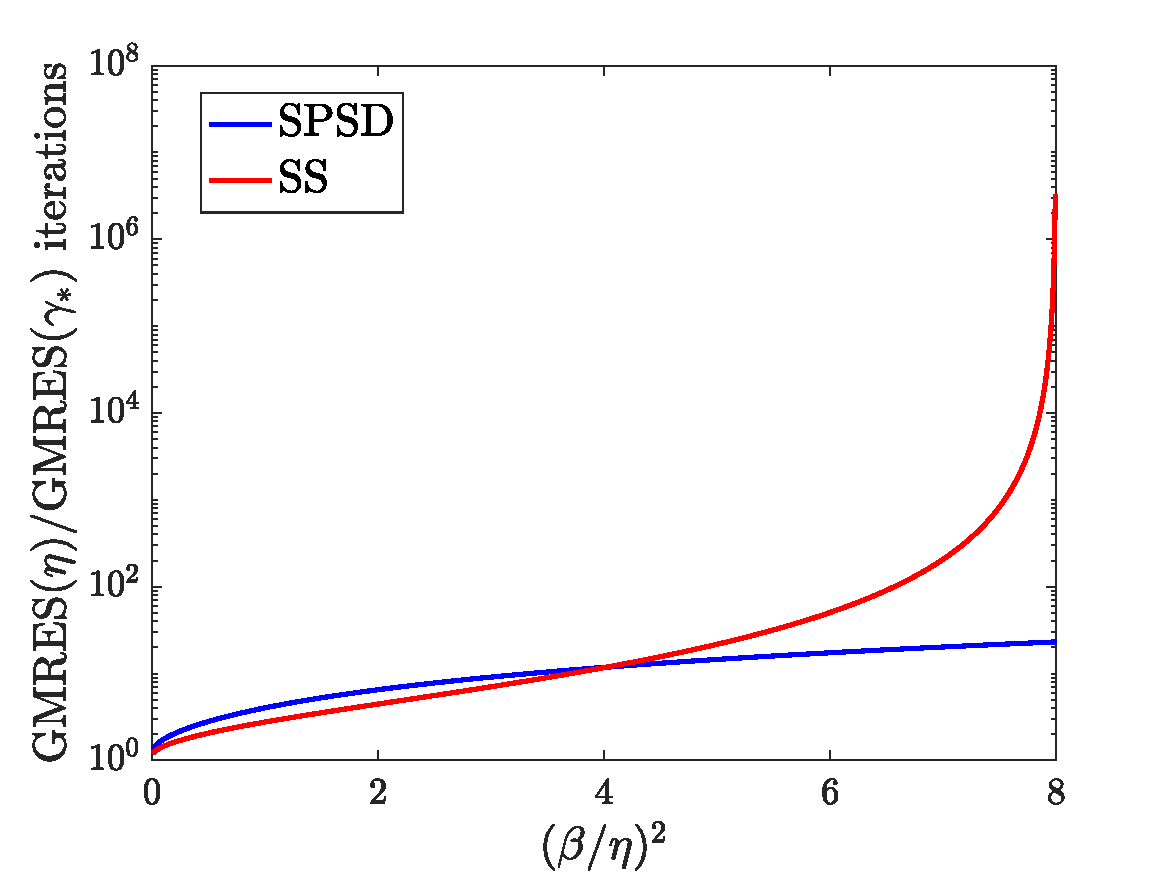
\includegraphics[width=0.575\textwidth]{figures/gmres_rel_iters_spsd_ss}
}
\caption{Approximate number of GMRES iterations \eqref{eq:gmres_approx_iters} based on convergence bounds \eqref{eq:gmres_eig_bound}, and solving to a relative tolerance of $10^{-12}$. \textbf{Left:} Absolute number of iterations for the convergence bounds plotted in Figure \ref{fig:gmres_bounds}. \textbf{Right:} Relative number of iterations for the SPSD and SS cases using $\gamma = \eta$ vs. $\gamma = \gamma_*$.}
\end{figure}

This predicted number of iterations results for this are shown in Figure \ref{fig:gmres_iters}. Notice first of all that the number of iterations for the SS $\gamma  = \eta$ case explodes as $(\beta/\eta)^2 \to 8$; we expected this however, from the earlier analysis since the symmetric component of ${\cal P}_{\gamma}$ becomes indefinite, and hence bound \eqref{eq:gmres_eig_bound} no longer holds. What I'd like to know is in this limit where GMRES \eqref{eq:gmres_eig_bound} breaks down, does it become less tight, or would be really see iteration growth qualitatively similar to that predicted in Figure \ref{fig:gmres_iters}.

From the right panel, we see this corresponds to a very large reduction in number of iterations when using $\gamma_*$ over $\eta$ when $(\beta/\eta)^2$ is large enough. Furthermore, there is a cross over point where the $\eta$ vs. $\gamma_*$ distinction becomes more important for the SS case compared to the SPSD case. 

Another observation: The reduction in iterations by a factor of $\sim$5--10 for the SPSD case is quite a bit larger than what we've observed in practice. For example, on this  $2 \times 2$ problem with linear diffusion, I got a reduction of 29 GMRES iterations to 15 at a value of $(\beta/\eta)^2 = 4.88$, so about a factor of 2. And this was using a relative stopping tolerance of $10^{-12}$, so the predicted number of iterations in the left-hand-side panel of $\sim$100 when using $\gamma_*$ is quite a bit too large...\\


I suppose I should just do some numerical tests to see if I get behaviour qualitatively similar to the right-hand-side of Figure \ref{fig:gmres_iters}.







% ---------------------------------------------------------------------------------------------- %
% ---------------------------------------------------------------------------------------------- %
\newpage
\subsection{General conditioning theory}

Consider the more general problem of the \tcb{right} preconditioning 
%
\begin{align}\nonumber
\mathcal{P}_\gamma :&=
S(\gamma I- \widehat{\mathcal{L}}_2)^{-1} \\
& = \left[ (\gamma I - \widehat{\mathcal{L}}_2) + (\eta-\gamma)I +
	\beta^2 (\eta I - \widehat{\mathcal{L}}_1)^{-1}\right]
	(\gamma I - \widehat{\mathcal{L}}_2)^{-1} \\
& = I - (\gamma - \eta)( \gamma I- \widehat{\mathcal{L}}_2)^{-1} + 
	\beta^2( \eta I-\widehat{\mathcal{L}}_1)^{-1}
	( \gamma I- \widehat{\mathcal{L}}_2)^{-1}\nonumber\\
& = I - \frac{\gamma - \eta}{\gamma} ( I- \tfrac{1}{\gamma}\widehat{\mathcal{L}}_2)^{-1} + 
	\frac{\beta^2}{\gamma\eta}( I- \tfrac{1}{\eta}\widehat{\mathcal{L}}_1)^{-1}
	( I- \tfrac{1}{\gamma}\widehat{\mathcal{L}}_2)^{-1},\label{eq:gamma2}
\end{align}




\begin{theorem}[Conditioning of preconditioned operator]\label{th:cond}
Suppose Assumptions \ref{ass:eig} and \ref{ass:fov} hold, that is, $\eta > 0$
and $W(\mathcal{L}) \leq 0$ \eqref{eq:fov}. Additionally, assume that
$\langle\mathcal{L}_1\mathbf{w},\mathcal{L}_2\mathbf{w}\rangle\geq 0$.
Let $\mathcal{P}_\gamma$ denote the right-preconditioned Schur complement,
with preconditioner $(\gamma I - \widehat{\mathcal{L}}_2)^{-1}$, for
$\gamma >\eta$, and define $\gamma_* := \tfrac{\eta^2+\beta^2}{\eta}$.
Then
\begin{align}\label{eq:gammastar}
\textnormal{cond}(\mathcal{P}_{\gamma_*}) \leq 
	2 + \frac{\beta^2}{\eta^2}.
\end{align}
\end{theorem}
\begin{proof}
Recall for matrix $A$, cond$(A) = \|A\|\|A^{-1}\|$.
First, consider bounding $\|(\gamma I- \widehat{\mathcal{L}}_2)^{-1}S\|$ for
$\gamma \geq \eta$:
%
\begin{align}\nonumber
\|\mathcal{P}_\gamma\| & = \left\| I - \frac{\gamma - \eta}{\gamma}
	( I- \tfrac{1}{\gamma}\widehat{\mathcal{L}}_2)^{-1} + 
	\frac{\beta^2}{\gamma\eta}( I- \tfrac{1}{\eta}\widehat{\mathcal{L}}_1)^{-1}
	( I- \tfrac{1}{\gamma}\widehat{\mathcal{L}}_2)^{-1} \right\| \\
% & \leq \left\| I - 2\frac{\gamma-\eta}
% 	{\gamma}\left(I - \tfrac{1}{\gamma}\mathcal{L}\right)^{-1}\right\| +
% 		\frac{\beta^2 + (\gamma-\eta)^2}{\gamma^2}\left\|
% 		\left(I - \tfrac{1}{\gamma}\mathcal{L}\right)^{-2} \right\| \\
& \leq \left\| I - \frac{\gamma-\eta}
	{\gamma}\left(I - \tfrac{1}{\gamma}\mathcal{L}_2\right)^{-1}\right\| +
		\frac{\beta^2}{\gamma\eta}
		\left\|( I- \tfrac{1}{\eta}\widehat{\mathcal{L}}_1)^{-1} \right\|
		\left\|( I- \tfrac{1}{\gamma}\widehat{\mathcal{L}}_2)^{-1}\right\|\nonumber \\
& \leq \left\| I - \frac{\gamma-\eta}
	{\gamma}\left(I - \tfrac{1}{\gamma}\mathcal{L}_2\right)^{-1}\right\| +
		\frac{\beta^2}{\gamma\eta}. \label{eq:Pgn}
\end{align}
%
For the first term, note that maximizing over $\mathbf{v}\in\mathbb{R}^n$ and
letting $\mathbf{v} := (I - \tfrac{1}{\gamma}\mathcal{L}_2)\mathbf{w}$,
%
\begin{align*}
\left\| I - \tfrac{\gamma-\eta}
	{\gamma}(I - \tfrac{1}{\gamma}\mathcal{L}_2)^{-1}\right\|^2
		& = \sup_{\mathbf{v}\neq\mathbf{0}} \frac{\left\| [I - \frac{\gamma-\eta}
	{\gamma}(I - \tfrac{1}{\gamma}\mathcal{L}_2)^{-1}]\mathbf{v}\right\|^2}{\|\mathbf{v}\|^2} 
= \sup_{\mathbf{w}\neq\mathbf{0}} \frac{\left\| (I - \tfrac{1}{\gamma}\mathcal{L}_2 -
		\frac{\gamma-\eta}{\gamma}I )\mathbf{w}\right\|^2}{\|(I - \tfrac{1}{\gamma}\mathcal{L}_2)
		\mathbf{w}\|^2} \\
% & = \sup_{\mathbf{w}\neq\mathbf{0}} \frac{\left\|[(1 - 2\frac{\gamma-\eta}{\gamma})
% 	I - \tfrac{1}{\gamma}\mathcal{L}_2]\mathbf{w}\right\|^2}{\|(I - \tfrac{1}{\gamma}\mathcal{L}_2)
% 		\mathbf{w}\|^2} \\
&\hspace{-5ex} = \sup_{\mathbf{w}\neq\mathbf{0}} \frac{(\tfrac{\eta}{\gamma})^2\|\mathbf{w}\|^2
	- \tfrac{\eta}{\gamma^2}\langle (\mathcal{L}_2 + \mathcal{L}_2^T)
		\mathbf{w},\mathbf{w}\rangle + \tfrac{1}{\gamma}^2\|\mathcal{L}_2\mathbf{w}\|^2}
	{\|\mathbf{w}\|^2 - \tfrac{1}{\gamma}\langle (\mathcal{L}_2 + \mathcal{L}_2^T)
		\mathbf{w},\mathbf{w}\rangle + \tfrac{1}{\gamma}^2\|\mathcal{L}_2\mathbf{w}\|^2}.
\end{align*}
%
Note that by assumption, $\gamma \geq \eta$, which implies
$0< \tfrac{\eta}{\gamma^2} \leq \tfrac{\eta^2}{\gamma^2}  < 1$, and 
$|1 - 2\tfrac{\gamma-\eta}{\gamma}| < 1$. In addition, we assume $W(\mathcal{L}_2)\leq 0$,
which implies $-\langle (\mathcal{L}_2+\mathcal{L}_2^T)\mathbf{w},\mathbf{w}\rangle \geq 0$
(see \Cref{th:fov}). It follows that all terms in the numerator and denominator are
positive, and
%
\begin{align} \label{eq:P1}
\left\| I - \tfrac{\gamma-\eta}
	{\gamma}(I - \tfrac{1}{\gamma}\mathcal{L}_2)^{-1}\right\|^2
& < \sup_{\mathbf{w}\neq\mathbf{0}} \frac{\|\mathbf{w}\|^2
	- \tfrac{1}{\gamma}\langle (\mathcal{L}_2 + \mathcal{L}_2^T)
		\mathbf{w},\mathbf{w}\rangle + \tfrac{1}{\gamma}^2\|\mathcal{L}_2\mathbf{w}\|^2}
	{\|\mathbf{w}\|^2 - \tfrac{1}{\gamma}\langle (\mathcal{L}_2 + \mathcal{L}^T)
		\mathbf{w},\mathbf{w}\rangle + \tfrac{1}{\gamma}^2\|\mathcal{L}\mathbf{w}\|^2} 
= 1.
\end{align}
%
Combining \eqref{eq:P0} and \eqref{eq:P1} yields
%
\begin{align}\label{eq:Pgamma_gen}
\|\mathcal{P}_\gamma\| \leq 1 + \frac{\beta^2}{\gamma\eta}.
\end{align}

Now consider bounding $\|\mathcal{P}_\gamma^{-1}\|$ from above. Let $s_{\max}(A)$
and $s_{\min}(A)$ denote the maximum and minimum singular value of matrix $A$,
respectively, and recall
%
\begin{align*}
\|\mathcal{P}_\gamma^{-1}\| = s_{\max}(\mathcal{P}_\gamma^{-1})
	& = \frac{1}{s_{\min}(\mathcal{P}_\gamma)}, \hspace{5ex}\textnormal{where}\hspace{2ex}
s_{\min}(\mathcal{P}_\gamma) =
	\min_{\mathbf{v}\neq\mathbf{0}} \frac{\|\mathcal{P}_\gamma\mathbf{v}\|}{\|\mathbf{v}\|}.
\end{align*}
%
Thus, consider the minimum singular value of $\mathcal{P}_\gamma$. Letting $\mathbf{v} :=
(I - \tfrac{1}{\gamma}\mathcal{L}_2)(I - \tfrac{1}{\eta}\mathcal{L}_1)\mathbf{w}$,
%
\begin{align}\nonumber
s_{\min}(\mathcal{P}_\gamma)^2 & = \min_{\mathbf{v}\neq\mathbf{0}}
	\frac{\left\| \left[I - \frac{\gamma - \eta}{\gamma}
	( I- \tfrac{1}{\gamma}\widehat{\mathcal{L}}_2)^{-1} + 
	\frac{\beta^2}{\gamma\eta}( I- \tfrac{1}{\eta}\widehat{\mathcal{L}}_1)^{-1}
	( I- \tfrac{1}{\gamma}\widehat{\mathcal{L}}_2)^{-1}\right]\mathbf{v} \right\|^2}
	{\|\mathbf{v}\|^2} \\
& = \min_{\mathbf{w}\neq\mathbf{0}}
	\frac{\left\| \left[(I - \tfrac{1}{\gamma}\mathcal{L}_2)(I - \tfrac{1}{\eta}\mathcal{L}_1)
		- \frac{\gamma-\eta}{\gamma}(I - \tfrac{1}{\eta} \mathcal{L}_1) +
		\frac{\beta^2}{\gamma\eta} I\right]\mathbf{w} \right\|^2}
	{\|(I - \tfrac{1}{\gamma}\mathcal{L}_2)(I - \tfrac{1}{\eta}\mathcal{L}_1)\mathbf{w}\|^2} \nonumber\\
& = \min_{\mathbf{w}\neq\mathbf{0}}
	\frac{\left\| \left[(I - \tfrac{1}{\gamma}\mathcal{L}_2)(I - \tfrac{1}{\eta}\mathcal{L}_1)
		+ \frac{\gamma-\eta}{\gamma\eta}\mathcal{L}_1 +
		\frac{\beta^2+\eta^2 - \gamma\eta}{\gamma\eta} I\right]\mathbf{w} \right\|^2}
	{\|(I - \tfrac{1}{\gamma}\mathcal{L}_2)(I - \tfrac{1}{\eta}\mathcal{L}_1)\mathbf{w}\|^2} \nonumber
\end{align}
%
Let us make the strategic choice of picking $\gamma$ such that the identity perturbation
$\tfrac{\beta^2+\eta^2 - \gamma\eta}{\gamma\eta} I = \mathbf{0}$, given by $\gamma_*
:= \tfrac{\eta^2+\beta^2}{\eta}$. Note, this is exactly the optimal $\gamma$ in the case
of SPD operators $\mathcal{L}$. Expanding, we have
%
\begin{align}
s_{\min}(\mathcal{P}_\gamma)^2 & = 
	\min_{\mathbf{w}\neq\mathbf{0}}
	\frac{\left\| \left[(I - \tfrac{1}{\gamma}\mathcal{L}_2)(I - \tfrac{1}{\eta}\mathcal{L}_1)
		+ \frac{\beta^2}{\eta(\eta^2+\beta^2)}\mathcal{L}_1\right]\mathbf{w} \right\|^2}
	{\|(I - \tfrac{1}{\gamma}\mathcal{L}_2)(I - \tfrac{1}{\eta}\mathcal{L}_1)\mathbf{w}\|^2} \nonumber\\
& = \min_{\mathbf{w}\neq\mathbf{0}} 1 +
	\frac{\beta^2}{\eta(\eta^2+\beta^2)}\cdot 
	\frac{\frac{\beta^2}{\eta(\eta^2+\beta^2)}\left\|\mathcal{L}_1\mathbf{w} \right\|^2
		+ 2\left\langle(I - \tfrac{1}{\gamma}\mathcal{L}_2)(I - \tfrac{1}{\eta}\mathcal{L}_1)\mathbf{w},
		\mathcal{L}_1\mathbf{w} \right\rangle}
	{\|(I - \tfrac{1}{\gamma}\mathcal{L}_2)(I - \tfrac{1}{\eta}\mathcal{L}_1)\mathbf{w}\|^2} \nonumber\\
& = 1 - \frac{\beta^2}{\eta^2+\beta^2} \cdot\max_{\mathbf{w}\neq\mathbf{0}}
	\frac{(-\tfrac{2}{\eta})\left\langle(I - \tfrac{1}{\gamma}\mathcal{L}_2)(I -
		\tfrac{1}{\eta}\mathcal{L}_1)\mathbf{w},
		\mathcal{L}_1\mathbf{w} \right\rangle- 
		\frac{\beta^2}{\eta^2(\eta^2+\beta^2)}\left\|\mathcal{L}_1\mathbf{w} \right\|^2}
	{\|(I - \tfrac{1}{\gamma}\mathcal{L}_2)(I - \tfrac{1}{\eta}\mathcal{L}_1)\mathbf{w}\|^2}.
	\label{eq:gen_smin}
\end{align}
%
Expanding the numerator term, we have
\begin{align}\nonumber
& (-\tfrac{2}{\eta})\left\langle(I - \tfrac{1}{\gamma}\mathcal{L}_2)(I - \tfrac{1}{\eta}\mathcal{L}_1)\mathbf{w},
		\mathcal{L}_1\mathbf{w} \right\rangle- 
		\frac{\beta^2}{\eta^2(\eta^2+\beta^2)}\left\|\mathcal{L}_1\mathbf{w} \right\|^2 \\
& = \left(\frac{2}{\eta^2} - \frac{\beta^2}{\eta^2(\eta^2+\beta^2)}\right)
			\left\|\mathcal{L}_1\mathbf{w} \right\|^2
		- \frac{2}{\eta}\langle\mathbf{w},\mathcal{L}_1\mathbf{w}\rangle
		- \frac{2}{\gamma\eta^2}\langle\mathcal{L}_2(\mathcal{L}_1\mathbf{w}),\mathcal{L}_1\mathbf{w}\rangle
		+ \frac{2}{\gamma\eta}\langle\mathcal{L}_1\mathbf{w},\mathcal{L}_2\mathbf{w}\rangle \nonumber\\
& = \left(\frac{1}{\eta^2} + \frac{1}{\eta^2+\beta^2}\right)
			\left\|\mathcal{L}_1\mathbf{w} \right\|^2
		- \frac{2}{\eta}\langle\mathbf{w},\mathcal{L}_1\mathbf{w}\rangle
		- \frac{2}{\gamma\eta^2}\langle\mathcal{L}_2(\mathcal{L}_1\mathbf{w}),\mathcal{L}_1\mathbf{w}\rangle
		+ \frac{2}{\gamma\eta}\langle\mathcal{L}_1\mathbf{w},\mathcal{L}_2\mathbf{w}\rangle.
		\label{eq:num_gen}
\end{align}
%
Now consider the denominator:
%
\begin{align}
\left\|(I - \tfrac{1}{\gamma}\mathcal{L}_2)(I - \tfrac{1}{\eta}\mathcal{L}_1)\mathbf{w}\right\|^2
& = \left\|\left(I + \tfrac{1}{\gamma\eta}\mathcal{L}_2\mathcal{L}_1\right)\mathbf{w} - 
	\left(\tfrac{1}{\gamma}\mathcal{L}_2 + \tfrac{1}{\eta}\mathcal{L}_1\right)\mathbf{w}\right\|^2 \nonumber\\
& = \left\|\left(I + \tfrac{1}{\gamma\eta}\mathcal{L}_2\mathcal{L}_1\right)\mathbf{w}\right\|^2
	+ \frac{1}{\gamma^2}\|\mathcal{L}_2\mathbf{w}\|^2
	+ \frac{1}{\eta^2}\|\mathcal{L}_1\mathbf{w}\|^2
	+ \frac{2}{\gamma\eta}\langle\mathcal{L}_1\mathbf{w},\mathcal{L}_2\mathbf{w}\rangle
	\nonumber\\ & \hspace{5ex}
	- \frac{2}{\gamma}\Big\langle \left(I + \tfrac{1}{\gamma\eta}\mathcal{L}_2\mathcal{L}_1\right)\mathbf{w},
		\mathcal{L}_2\mathbf{w}\Big\rangle
	- \frac{2}{\eta}\Big\langle \left(I + \tfrac{1}{\gamma\eta}\mathcal{L}_2\mathcal{L}_1\right)\mathbf{w},
		\mathcal{L}_1\mathbf{w}\Big\rangle \nonumber\\
& \geq \left\|\left(I + \tfrac{1}{\gamma\eta}\mathcal{L}_2\mathcal{L}_1\right)\mathbf{w}\right\|^2
	+ \frac{1}{\gamma^2}\|\mathcal{L}_2\mathbf{w}\|^2
	+ \frac{1}{\eta^2}\|\mathcal{L}_1\mathbf{w}\|^2
	+ \frac{2}{\gamma\eta}\langle\mathcal{L}_1\mathbf{w},\mathcal{L}_2\mathbf{w}\rangle
	\nonumber\\ & \hspace{5ex}
	- \frac{2}{\gamma}\left\| \left(I + \tfrac{1}{\gamma\eta}\mathcal{L}_2\mathcal{L}_1\right)\mathbf{w}\right\|
		\left\|\mathcal{L}_2\mathbf{w}\right\|
	- \frac{2}{\eta}\Big\langle \left(I + \tfrac{1}{\gamma\eta}\mathcal{L}_2\mathcal{L}_1\right)\mathbf{w},
		\mathcal{L}_1\mathbf{w}\Big\rangle \nonumber\\
& = \left( \left\|\left(I + \tfrac{1}{\gamma\eta}\mathcal{L}_2\mathcal{L}_1\right)\mathbf{w}\right\|
		- \frac{1}{\gamma}\|\mathcal{L}_2\mathbf{w}\|\right)^2
	+ \frac{1}{\eta^2}\|\mathcal{L}_1\mathbf{w}\|^2
	\nonumber\\ & \hspace{5ex}
	- \frac{2}{\eta}\Big\langle \left(I + \tfrac{1}{\gamma\eta}\mathcal{L}_2\mathcal{L}_1\right)\mathbf{w},
		\mathcal{L}_1\mathbf{w}\Big\rangle
	+ \frac{2}{\gamma\eta}\langle\mathcal{L}_1\mathbf{w},\mathcal{L}_2\mathbf{w}\rangle \nonumber\\
& \geq \frac{1}{\eta^2}\|\mathcal{L}_1\mathbf{w}\|^2
	- \frac{2}{\eta}\langle \mathbf{w}, \mathcal{L}_1\mathbf{w}\Big\rangle 
	- \frac{2}{\gamma\eta^2}\langle \mathcal{L}_2(\mathcal{L}_1\mathbf{w}),
		\mathcal{L}_1\mathbf{w}\Big\rangle
	+ \frac{2}{\gamma\eta}\langle\mathcal{L}_1\mathbf{w},\mathcal{L}_2\mathbf{w}\rangle.
		\label{eq:den_gen}
\end{align}
%

By assumption $\langle\mathcal{L}_1\mathbf{w},\mathcal{L}_2\mathbf{w}\rangle\geq 0$,
and thus all terms in \eqref{eq:num_gen} and \eqref{eq:den_gen} are non-negative.
Returning to the minimum singular value defined in \eqref{eq:gen_smin} and plugging in
the numerator \eqref{eq:num_gen} and denominator bounds \eqref{eq:den_gen} yields
an upper bound on the maximum over $\mathbf{w}$,
%
\begin{align*}
&\hspace{-5ex} \max_{\mathbf{w}\neq\mathbf{0}}
	\frac{(-\tfrac{2}{\eta})\left\langle(I - \tfrac{1}{\gamma}\mathcal{L}_2)(I -
		\tfrac{1}{\eta}\mathcal{L}_1)\mathbf{w},
		\mathcal{L}_1\mathbf{w} \right\rangle- 
		\frac{\beta^2}{\eta^2(\eta^2+\beta^2)}\left\|\mathcal{L}_1\mathbf{w} \right\|^2}
	{\|(I - \tfrac{1}{\gamma}\mathcal{L}_2)(I - \tfrac{1}{\eta}\mathcal{L}_1)\mathbf{w}\|^2} \\
& \leq \max_{\mathbf{w}\neq\mathbf{0}}\frac{\left(\frac{1}{\eta^2} + \frac{1}{\eta^2+\beta^2)}\right)
			\left\|\mathcal{L}_1\mathbf{w} \right\|^2
		- \frac{2}{\eta}\langle\mathbf{w},\mathcal{L}_1\mathbf{w}\rangle
		- \frac{2}{\gamma\eta^2}\langle\mathcal{L}_2(\mathcal{L}_1\mathbf{w}),\mathcal{L}_1\mathbf{w}\rangle
		+ \frac{2}{\gamma\eta}\langle\mathcal{L}_1\mathbf{w},\mathcal{L}_2\mathbf{w}\rangle}
	{\frac{1}{\eta^2}\|\mathcal{L}_1\mathbf{w}\|^2
	- \frac{2}{\eta}\langle \mathbf{w}, \mathcal{L}_1\mathbf{w}\Big\rangle 
	- \frac{2}{\gamma\eta^2}\langle \mathcal{L}_2(\mathcal{L}_1\mathbf{w}),
		\mathcal{L}_1\mathbf{w}\Big\rangle
	+ \frac{2}{\gamma\eta}\langle\mathcal{L}_1\mathbf{w},\mathcal{L}_2\mathbf{w}\rangle} \nonumber\\
& \leq \frac{\frac{1}{\eta^2} + \frac{1}{\eta^2+\beta^2)}}{\frac{1}{\eta^2}} \\
& = \frac{2\eta^2 + \beta^2}{\eta^2+\beta^2}.
\end{align*}
%
Plugging in to \eqref{eq:gen_smin} yields
%
\begin{align}
s_{\min}(\mathcal{P}_{\gamma_*})^2 &\geq 1 - \frac{\beta^2}{\eta^2+\beta^2}
	\frac{2\eta^2 + \beta^2}{\eta^2+\beta^2}
= \frac{\eta^4}{(\eta^2+\beta^2)^2}.
\end{align}
%
Combing with \eqref{eq:Pgamma_gen} yields
%
\begin{align}
\textnormal{cond}(\mathcal{P}_{\gamma_*}) = \|\mathcal{P}_{\gamma_*}\|\|\mathcal{P}_{\gamma_*}^{-1}\|
	\leq \left(1+\frac{\eta^2}{\eta^2+\beta^2}\right)\frac{\eta^2+\beta^2}{\eta^2}
	= 2+\frac{\beta^2}{\eta^2},
\end{align}
%
which completes the proof.
\end{proof}
%


% ---------------------------------------------------------------------------------------------- %
% ---------------------------------------------------------------------------------------------- %
\subsection{Block conditioning theory: $\mathcal{L}_1 = \mathcal{L}_2$}
%
\begin{theorem}[Conditioning of preconditioned operator]\label{th:cond}
Suppose Assumptions \ref{ass:eig} and \ref{ass:fov} hold, that is, $\eta > 0$
and $W(\widehat{\mathcal{L}}),W(\widehat{\mathcal{L}}) \leq 0$ \eqref{eq:fov}.
Additionally, assume that $\langle\widehat{\mathcal{L}}\mathbf{w},
\widehat{\mathcal{L}}\mathbf{w}\rangle\geq 0$. Let $\mathcal{P}_\gamma$
denote the right-preconditioned Schur complement \eqref{eq:gamma2}, with
preconditioner $(\gamma I - \widehat{\mathcal{L}})^{-1}$, for $\gamma >\eta$,
and define $\gamma_* := \tfrac{\eta^2+\beta^2}{\eta}$. Then
\begin{align}\label{eq:gammastar_cond}
\textnormal{cond}(\mathcal{P}_{\gamma_*}) \leq 
	2 + \frac{\beta^2}{\eta^2}.
\end{align}
\end{theorem}
\begin{proof}
Recall for matrix $A$, cond$(A) = \|A\|\|A^{-1}\|$.
First, consider bounding $\|(\gamma I- \widehat{\mathcal{L}})^{-1}S\|$ for
$\gamma \geq \eta$:
%
\begin{align}\nonumber
\|\mathcal{P}_\gamma\| & = \left\| I - \frac{\gamma - \eta}{\gamma}
	( I- \tfrac{1}{\gamma}\widehat{\mathcal{L}})^{-1} + 
	\frac{\beta^2}{\gamma\eta}( I- \tfrac{1}{\eta}\widehat{\mathcal{L}})^{-1}
	( I- \tfrac{1}{\gamma}\widehat{\mathcal{L}})^{-1} \right\| \\
% & \leq \left\| I - 2\frac{\gamma-\eta}
% 	{\gamma}\left(I - \tfrac{1}{\gamma}\widehat{\mathcal{L}}\right)^{-1}\right\| +
% 		\frac{\beta^2 + (\gamma-\eta)^2}{\gamma^2}\left\|
% 		\left(I - \tfrac{1}{\gamma}\widehat{\mathcal{L}}\right)^{-2} \right\| \\
& \leq \left\| I - \frac{\gamma-\eta}
	{\gamma}\left(I - \tfrac{1}{\gamma}\widehat{\mathcal{L}}\right)^{-1}\right\| +
		\frac{\beta^2}{\gamma\eta}
		\left\|( I- \tfrac{1}{\eta}\widehat{\mathcal{L}})^{-1} \right\|
		\left\|( I- \tfrac{1}{\gamma}\widehat{\mathcal{L}})^{-1}\right\|\nonumber \\
& \leq \left\| I - \frac{\gamma-\eta}
	{\gamma}\left(I - \tfrac{1}{\gamma}\widehat{\mathcal{L}}\right)^{-1}\right\| +
		\frac{\beta^2}{\gamma\eta}. \label{eq:Pgn}
\end{align}
%
For the first term, note that maximizing over $\mathbf{v}\in\mathbb{R}^n$ and
letting $\mathbf{v} := (I - \tfrac{1}{\gamma}\widehat{\mathcal{L}})\mathbf{w}$,
%
\begin{align*}
\left\| I - \tfrac{\gamma-\eta}
	{\gamma}(I - \tfrac{1}{\gamma}\widehat{\mathcal{L}})^{-1}\right\|^2
		& = \sup_{\mathbf{v}\neq\mathbf{0}} \frac{\left\| [I - \frac{\gamma-\eta}
	{\gamma}(I - \tfrac{1}{\gamma}\widehat{\mathcal{L}})^{-1}]\mathbf{v}\right\|^2}{\|\mathbf{v}\|^2}  \\
& = \sup_{\mathbf{w}\neq\mathbf{0}} \frac{\left\| (I - \tfrac{1}{\gamma}\widehat{\mathcal{L}} -
		\frac{\gamma-\eta}{\gamma}I )\mathbf{w}\right\|^2}{\|(I - \tfrac{1}{\gamma}\widehat{\mathcal{L}})
		\mathbf{w}\|^2} \\
% & = \sup_{\mathbf{w}\neq\mathbf{0}} \frac{\left\|[(1 - 2\frac{\gamma-\eta}{\gamma})
% 	I - \tfrac{1}{\gamma}\widehat{\mathcal{L}}]\mathbf{w}\right\|^2}{\|(I - \tfrac{1}{\gamma}\widehat{\mathcal{L}})
% 		\mathbf{w}\|^2} \\
& = \sup_{\mathbf{w}\neq\mathbf{0}} \frac{(\tfrac{\eta}{\gamma})^2\|\mathbf{w}\|^2
	- \tfrac{\eta}{\gamma^2}\langle (\widehat{\mathcal{L}} + \widehat{\mathcal{L}}^T)
		\mathbf{w},\mathbf{w}\rangle + \tfrac{1}{\gamma}^2\|\widehat{\mathcal{L}}\mathbf{w}\|^2}
	{\|\mathbf{w}\|^2 - \tfrac{1}{\gamma}\langle (\widehat{\mathcal{L}} + \widehat{\mathcal{L}}^T)
		\mathbf{w},\mathbf{w}\rangle + \tfrac{1}{\gamma}^2\|\widehat{\mathcal{L}}\mathbf{w}\|^2}.
\end{align*}
%
Note that by assumption, $\gamma \geq \eta$, which implies
$0< \tfrac{\eta}{\gamma^2} \leq \tfrac{\eta^2}{\gamma^2}  < 1$, and 
$|1 - 2\tfrac{\gamma-\eta}{\gamma}| < 1$. In addition, by \Cref{ass:fov} $W(\widehat{\mathcal{L}})\leq 0$,
which implies $-\langle (\widehat{\mathcal{L}}+\widehat{\mathcal{L}}^T)\mathbf{w},\mathbf{w}\rangle \geq 0$
\cite{gustafson1997numerical,mees1979domains}.
It follows that all terms in the numerator and denominator are positive, and
%
\begin{align} \label{eq:P1}
\left\| I - \tfrac{\gamma-\eta}
	{\gamma}(I - \tfrac{1}{\gamma}\widehat{\mathcal{L}})^{-1}\right\|^2
& < \sup_{\mathbf{w}\neq\mathbf{0}} \frac{\|\mathbf{w}\|^2
	- \tfrac{1}{\gamma}\langle (\widehat{\mathcal{L}} + \widehat{\mathcal{L}}^T)
		\mathbf{w},\mathbf{w}\rangle + \tfrac{1}{\gamma}^2\|\widehat{\mathcal{L}}\mathbf{w}\|^2}
	{\|\mathbf{w}\|^2 - \tfrac{1}{\gamma}\langle (\widehat{\mathcal{L}} + \widehat{\mathcal{L}}^T)
		\mathbf{w},\mathbf{w}\rangle + \tfrac{1}{\gamma}^2\|\widehat{\mathcal{L}}\mathbf{w}\|^2} 
= 1.
\end{align}
%
Combining \eqref{eq:Pgn} and \eqref{eq:P1} yields
%
\begin{align}\label{eq:Pgamma_gen}
\|\mathcal{P}_\gamma\| \leq 1 + \frac{\beta^2}{\gamma\eta}.
\end{align}

Now consider bounding $\|\mathcal{P}_\gamma^{-1}\|$ from above. Let $s_{\max}(A)$
and $s_{\min}(A)$ denote the maximum and minimum singular value of matrix $A$,
respectively, and recall
%
\begin{align}\label{eq:sing_vals}
\|\mathcal{P}_\gamma^{-1}\| = s_{\max}(\mathcal{P}_\gamma^{-1})
	& = \frac{1}{s_{\min}(\mathcal{P}_\gamma)}, \hspace{5ex}\textnormal{where}\hspace{2ex}
s_{\min}(\mathcal{P}_\gamma) =
	\min_{\mathbf{v}\neq\mathbf{0}} \frac{\|\mathcal{P}_\gamma\mathbf{v}\|}{\|\mathbf{v}\|}.
\end{align}
%
Thus, consider the minimum singular value of $\mathcal{P}_\gamma$. Letting $\mathbf{v} :=
(I - \tfrac{1}{\gamma}\widehat{\mathcal{L}})(I - \tfrac{1}{\eta}\widehat{\mathcal{L}})\mathbf{w}$,
%
\begin{align}\nonumber
s_{\min}(\mathcal{P}_\gamma)^2 & = \min_{\mathbf{v}\neq\mathbf{0}}
	\frac{\left\| \left[I - \frac{\gamma - \eta}{\gamma}
	( I- \tfrac{1}{\gamma}\widehat{\mathcal{L}})^{-1} + 
	\frac{\beta^2}{\gamma\eta}( I- \tfrac{1}{\eta}\widehat{\mathcal{L}})^{-1}
	( I- \tfrac{1}{\gamma}\widehat{\mathcal{L}})^{-1}\right]\mathbf{v} \right\|^2}
	{\|\mathbf{v}\|^2} \\
& = \min_{\mathbf{w}\neq\mathbf{0}}
	\frac{\left\| \left[(I - \tfrac{1}{\gamma}\widehat{\mathcal{L}})(I - \tfrac{1}{\eta}\widehat{\mathcal{L}})
		- \frac{\gamma-\eta}{\gamma}(I - \tfrac{1}{\eta} \widehat{\mathcal{L}}) +
		\frac{\beta^2}{\gamma\eta} I\right]\mathbf{w} \right\|^2}
	{\|(I - \tfrac{1}{\gamma}\widehat{\mathcal{L}})(I - \tfrac{1}{\eta}\widehat{\mathcal{L}})\mathbf{w}\|^2} \nonumber\\
& = \min_{\mathbf{w}\neq\mathbf{0}}
	\frac{\left\| \left[(I - \tfrac{1}{\gamma}\widehat{\mathcal{L}})(I - \tfrac{1}{\eta}\widehat{\mathcal{L}})
		+ \frac{\gamma-\eta}{\gamma\eta}\widehat{\mathcal{L}} +
		\frac{\beta^2+\eta^2 - \gamma\eta}{\gamma\eta} I\right]\mathbf{w} \right\|^2}
	{\|(I - \tfrac{1}{\gamma}\widehat{\mathcal{L}})(I - \tfrac{1}{\eta}\widehat{\mathcal{L}})\mathbf{w}\|^2} \nonumber
\end{align}
%
Let us make the strategic choice of picking $\gamma$ such that the identity perturbation
$\tfrac{\beta^2+\eta^2 - \gamma\eta}{\gamma\eta} I = \mathbf{0}$, given by $\gamma_*
:= \tfrac{\eta^2+\beta^2}{\eta}$. Note, this is exactly the optimal $\gamma$ derived 
in \Cref{sec:theory:spd}. Expanding, we have
%
\begin{align}
& \hspace{-5ex}
s_{\min}(\mathcal{P}_\gamma)^2 = 
	\min_{\mathbf{w}\neq\mathbf{0}}
	\frac{\left\| \left[(I - \tfrac{1}{\gamma}\widehat{\mathcal{L}})(I - \tfrac{1}{\eta}\widehat{\mathcal{L}})
		+ \frac{\beta^2}{\eta(\eta^2+\beta^2)}\widehat{\mathcal{L}}\right]\mathbf{w} \right\|^2}
	{\|(I - \tfrac{1}{\gamma}\widehat{\mathcal{L}})(I - \tfrac{1}{\eta}\widehat{\mathcal{L}})\mathbf{w}\|^2} \nonumber\\
& = \min_{\mathbf{w}\neq\mathbf{0}} 1 +
	\frac{\beta^2}{\eta(\eta^2+\beta^2)}\cdot 
	\frac{\frac{\beta^2}{\eta(\eta^2+\beta^2)}\left\|\widehat{\mathcal{L}}\mathbf{w} \right\|^2
		+ 2\left\langle(I - \tfrac{1}{\gamma}\widehat{\mathcal{L}})(I - \tfrac{1}{\eta}\widehat{\mathcal{L}})\mathbf{w},
		\widehat{\mathcal{L}}\mathbf{w} \right\rangle}
	{\|(I - \tfrac{1}{\gamma}\widehat{\mathcal{L}})(I - \tfrac{1}{\eta}\widehat{\mathcal{L}})\mathbf{w}\|^2} \nonumber\\
& = 1 - \frac{\beta^2}{\eta^2+\beta^2} \cdot\max_{\mathbf{w}\neq\mathbf{0}}
	\frac{(-\tfrac{2}{\eta})\left\langle(I - \tfrac{1}{\gamma}\widehat{\mathcal{L}})(I -
		\tfrac{1}{\eta}\widehat{\mathcal{L}})\mathbf{w},
		\widehat{\mathcal{L}}\mathbf{w} \right\rangle- 
		\frac{\beta^2}{\eta^2(\eta^2+\beta^2)}\left\|\widehat{\mathcal{L}}\mathbf{w} \right\|^2}
	{\|(I - \tfrac{1}{\gamma}\widehat{\mathcal{L}})(I - \tfrac{1}{\eta}\widehat{\mathcal{L}})\mathbf{w}\|^2}.
	\label{eq:gen_smin}
\end{align}
%
Expanding the numerator term, we have
{\small
\begin{align}\nonumber
& (-\tfrac{2}{\eta})\left\langle(I - \tfrac{1}{\gamma}\widehat{\mathcal{L}})(I -
	\tfrac{1}{\eta}\widehat{\mathcal{L}})\mathbf{w}, \widehat{\mathcal{L}}\mathbf{w} \right\rangle- 
		\frac{\beta^2}{\eta^2(\eta^2+\beta^2)}\left\|\widehat{\mathcal{L}}\mathbf{w} \right\|^2 \\
% & = \left(\frac{2}{\eta^2} - \frac{\beta^2}{\eta^2(\eta^2+\beta^2)}\right)
% 			\left\|\widehat{\mathcal{L}}\mathbf{w} \right\|^2
% 		- \frac{2}{\eta}\langle\mathbf{w},\widehat{\mathcal{L}}\mathbf{w}\rangle
% 		- \frac{2}{\gamma\eta^2}\langle\widehat{\mathcal{L}}(\widehat{\mathcal{L}}\mathbf{w}),\widehat{\mathcal{L}}\mathbf{w}\rangle
% 		+ \frac{2}{\gamma\eta}\langle\widehat{\mathcal{L}}\mathbf{w},\widehat{\mathcal{L}}\mathbf{w}\rangle \nonumber\\
& = \left(\frac{1}{\eta^2} + \frac{1}{\eta^2+\beta^2} + \frac{2}{\gamma\eta}\right)
			\left\|\widehat{\mathcal{L}}\mathbf{w} \right\|^2
		- \frac{2}{\eta}\langle\mathbf{w},\widehat{\mathcal{L}}\mathbf{w}\rangle
		- \frac{2}{\gamma\eta^2}\langle\widehat{\mathcal{L}}(\widehat{\mathcal{L}}\mathbf{w}),\widehat{\mathcal{L}}\mathbf{w}\rangle.
		\label{eq:num_gen}
\end{align}
}
%
Now consider the denominator:
%
\begin{align}
& \hspace{-10ex}
\left\|(I - \tfrac{1}{\gamma}\widehat{\mathcal{L}})(I - \tfrac{1}{\eta}\widehat{\mathcal{L}})\mathbf{w}\right\|^2
= \left\|\left(I + \tfrac{1}{\gamma\eta}\widehat{\mathcal{L}}^2\right)\mathbf{w} - 
	\tfrac{\gamma+\eta}{\gamma\eta}\widehat{\mathcal{L}}\mathbf{w}\right\|^2 \nonumber\\
& = \left\|\left(I + \tfrac{1}{\gamma\eta}\widehat{\mathcal{L}}^2\right)\mathbf{w}\right\|^2
	+ \frac{(\gamma+\eta)^2}{(\gamma\eta)^2}\|\widehat{\mathcal{L}}\mathbf{w}\|^2
	- \frac{2(\gamma+\eta)}{\gamma\eta}\langle \widehat{\mathcal{L}}\mathbf{w}, \mathbf{w}\rangle
	- \frac{2(\gamma+\eta)}{(\gamma\eta)^2}\langle \widehat{\mathcal{L}}(\widehat{\mathcal{L}}\mathbf{w}),
		\widehat{\mathcal{L}}\mathbf{w}\rangle \nonumber\\
& \geq \frac{(\gamma+\eta)^2}{(\gamma\eta)^2}\|\widehat{\mathcal{L}}\mathbf{w}\|^2
	- \frac{2(\gamma+\eta)}{\gamma\eta}\langle \widehat{\mathcal{L}}\mathbf{w}, \mathbf{w}\rangle
	- \frac{2(\gamma+\eta)}{(\gamma\eta)^2}\langle \widehat{\mathcal{L}}(\widehat{\mathcal{L}}\mathbf{w}),
		\widehat{\mathcal{L}}\mathbf{w}\rangle . \label{eq:den_gen}
\end{align}
%

Note that all terms in \eqref{eq:num_gen} and \eqref{eq:den_gen} are non-negative.
Returning to the minimum singular value defined in \eqref{eq:gen_smin} and plugging in
the numerator \eqref{eq:num_gen} and denominator bounds \eqref{eq:den_gen} yields
an upper bound on the maximum over $\mathbf{w}$,
%
\begin{align*}
&\max_{\mathbf{w}\neq\mathbf{0}}
	\frac{(-\tfrac{2}{\eta})\left\langle(I - \tfrac{1}{\gamma}\widehat{\mathcal{L}})(I -
		\tfrac{1}{\eta}\widehat{\mathcal{L}})\mathbf{w},
		\widehat{\mathcal{L}}\mathbf{w} \right\rangle- 
		\frac{\beta^2}{\eta^2(\eta^2+\beta^2)}\left\|\widehat{\mathcal{L}}\mathbf{w} \right\|^2}
	{\|(I - \tfrac{1}{\gamma}\widehat{\mathcal{L}})(I - \tfrac{1}{\eta}\widehat{\mathcal{L}})\mathbf{w}\|^2} \\
& \leq \max_{\mathbf{w}\neq\mathbf{0}}\frac{\left(\frac{1}{\eta^2} +
		\frac{1}{\eta^2+\beta^2} + \frac{2}{\gamma\eta}\right)
			\left\|\widehat{\mathcal{L}}\mathbf{w} \right\|^2
		- \frac{2}{\eta}\langle\mathbf{w},\widehat{\mathcal{L}}\mathbf{w}\rangle
		- \frac{2}{\gamma\eta^2}\langle\widehat{\mathcal{L}}(\widehat{\mathcal{L}}\mathbf{w}),\widehat{\mathcal{L}}\mathbf{w}\rangle}
	{\frac{(\gamma+\eta)^2}{(\gamma\eta)^2}\|\widehat{\mathcal{L}}\mathbf{w}\|^2
	- \frac{2(\gamma+\eta)}{\gamma\eta}\langle \widehat{\mathcal{L}}\mathbf{w}, \mathbf{w}\rangle
	- \frac{2(\gamma+\eta)}{(\gamma\eta)^2}\langle \widehat{\mathcal{L}}(\widehat{\mathcal{L}}\mathbf{w}),
		\widehat{\mathcal{L}}\mathbf{w}\rangle} \nonumber\\
& \leq \frac{\frac{1}{\eta^2} + \frac{1}{\eta^2+\beta^2}+ \frac{2}{\gamma\eta}}
	{\frac{(\gamma+\eta)^2}{(\gamma\eta)^2}} \\
& = \frac{\beta^4+5\beta^2\eta^2+4\eta^4}{\beta^4+4\beta^2\eta^2+4\eta^4}.
\end{align*}
%
Simplifying and plugging in to \eqref{eq:gen_smin} yields
%
\begin{align}\label{eq:smin_bound}
s_{\min}(\mathcal{P}_{\gamma_*})^2 &\geq 1 - \frac{\beta^2}{\eta^2+\beta^2} \cdot
	\frac{\beta^4+5\beta^2\eta^2+4\eta^4}{\beta^4+4\beta^2\eta^2+4\eta^4}
= \frac{4\eta^4}{(2\eta^2+\beta^2)^2}.
\end{align}
%
Applying \eqref{eq:sing_vals} to \eqref{eq:smin_bound} and
combining with \eqref{eq:Pgamma_gen} yields
%
\begin{align}
\textnormal{cond}(\mathcal{P}_{\gamma_*}) = \|\mathcal{P}_{\gamma_*}\|\|\mathcal{P}_{\gamma_*}^{-1}\|
	\leq \left(1+\frac{\eta^2}{\eta^2+\beta^2}\right)\frac{2\eta^2+\beta^2}{2\eta^2}
	= 2+\frac{\beta^2}{2\eta^2} - \frac{\beta^2}{2\eta^2+2\beta^2},
\end{align}
%
which completes the proof.
\end{proof}
%



% ---------------------------------------------------------------------------------------------- %
% ---------------------------------------------------------------------------------------------- %
\subsection{Better block conditioning theory: $\mathcal{L}_1 = \mathcal{L}_2$}

Here we use Oliver's approach to get a tighter bound.
Consider the more general problem of the \tcb{right} preconditioning 
%
\begin{align}\nonumber
\mathcal{P}_\gamma :&=
S(\gamma I- \widehat{\mathcal{L}}_2)^{-1} \\
& = \left[ (\gamma I - \widehat{\mathcal{L}}_2) + (\eta-\gamma)I +
	\beta^2 (\eta I - \widehat{\mathcal{L}}_1)^{-1}\right]
	(\gamma I - \widehat{\mathcal{L}}_2)^{-1} \\
& = I - (\gamma - \eta)( \gamma I- \widehat{\mathcal{L}}_2)^{-1} + 
	\beta^2( \eta I-\widehat{\mathcal{L}}_1)^{-1}
	( \gamma I- \widehat{\mathcal{L}}_2)^{-1}\nonumber
\end{align}
%
In considering $\|\mathcal{P}_\gamma\mathbf{w}\|/\|\mathbf{w}\|$, let $\mathbf{w}:= 
(\gamma I- \widehat{\mathcal{L}}_2)(\eta I-\widehat{\mathcal{L}}_1)\mathbf{v}$.
Then,
%
\begin{align*}
\mathcal{P}_\gamma\mathbf{w} & = \left[
	(\gamma I- \widehat{\mathcal{L}}_2)(\eta I-\widehat{\mathcal{L}}_1) ]
	 - (\gamma - \eta)(\eta I-\widehat{\mathcal{L}}_1) + \beta^2 I\right]\mathbf{v} \\
& = \left[\eta\gamma I - \eta\widehat{\mathcal{L}}_2 - \gamma \widehat{\mathcal{L}}_1
	+ \widehat{\mathcal{L}}_2\widehat{\mathcal{L}}_1 - \gamma\eta I + \eta^2 I
	+ \gamma \widehat{\mathcal{L}}_1 - \eta \widehat{\mathcal{L}}_1 + \beta^2\right]\mathbf{v} \\
& = \left[ (\eta^2+\beta^2) I - \eta (\widehat{\mathcal{L}}_1 + \widehat{\mathcal{L}}_2) +
	\widehat{\mathcal{L}}_2\widehat{\mathcal{L}}_1 \right]\mathbf{v}, \\
\mathbf{w} & = \left[ \gamma\eta I - \gamma\widehat{\mathcal{L}}_2 -
	\eta \widehat{\mathcal{L}}_1 +
	\widehat{\mathcal{L}}_2\widehat{\mathcal{L}}_1 \right]\mathbf{v}.
\end{align*}
%
For now, assume $ \widehat{\mathcal{L}}_1 = \widehat{\mathcal{L}}_2$. Then,
%
\begin{align*}
\mathcal{P}_\gamma\mathbf{w} & = \left[ (\eta^2+\beta^2) I - 2\eta \widehat{\mathcal{L}} +
	\widehat{\mathcal{L}}^2 \right]\mathbf{v}, \\
\mathbf{w} & = \left[ \eta\gamma I - (\eta+\gamma)\widehat{\mathcal{L}} +
	\widehat{\mathcal{L}}^2\right]\mathbf{v}.
\end{align*}
%
Then, 
%
\begin{align*}
\frac{\|\mathcal{P}_\gamma\mathbf{w}\|^2}{\|\mathbf{w}\|^2}
	& = \frac{\left\|\left[ (\eta^2+\beta^2) I - 2\eta \widehat{\mathcal{L}} +
	\widehat{\mathcal{L}}^2 \right]\mathbf{v}\right\|^2}
		{\left\|\left[ \eta\gamma I - (\eta+\gamma)\widehat{\mathcal{L}} +
	\widehat{\mathcal{L}}^2\right]\mathbf{v}\right\|^2 } \\
& = \frac{\left\| (\eta^2+\beta^2) \mathbf{v} + \widehat{\mathcal{L}}^2\mathbf{v}\right\|^2
	+ 4\eta^2\|\widehat{\mathcal{L}}\mathbf{v}\|^2 - 
	4\eta (\eta^2+\beta^2)\langle \widehat{\mathcal{L}}\mathbf{v},\mathbf{v}\rangle -
	4\eta \langle \widehat{\mathcal{L}}(\widehat{\mathcal{L}}\mathbf{v}),
		\widehat{\mathcal{L}}\mathbf{v}\rangle}
	{\left\| \eta\gamma \mathbf{v} + \widehat{\mathcal{L}}^2\mathbf{v}\right\|^2
	+ (\eta+\gamma)^2\|\widehat{\mathcal{L}}\mathbf{v}\|^2 -
	2(\eta+\gamma)\eta\gamma\langle \widehat{\mathcal{L}}\mathbf{v},\mathbf{v}\rangle -
	2(\eta+\gamma) \langle \widehat{\mathcal{L}}(\widehat{\mathcal{L}}\mathbf{v}),
		\widehat{\mathcal{L}}\mathbf{v}\rangle}
\end{align*}
%
Notice all terms in the numerator and denominator are nonnegative, with at least
one strictly positive. Making the strategic choice $\gamma = (\eta^2+\beta^2)/\eta$,
we get the simplification 
%
\begin{align*}
\frac{\|\mathcal{P}_\gamma\mathbf{w}\|^2}{\|\mathbf{w}\|^2}
& = \frac{\left\| (\eta^2+\beta^2) \mathbf{v} + \widehat{\mathcal{L}}^2\mathbf{v}\right\|^2
	+ 4\eta^2\|\widehat{\mathcal{L}}\mathbf{v}\|^2 - 
	4\eta (\eta^2+\beta^2)\langle \widehat{\mathcal{L}}\mathbf{v},\mathbf{v}\rangle -
	4\eta \langle \widehat{\mathcal{L}}(\widehat{\mathcal{L}}\mathbf{v}),
		\widehat{\mathcal{L}}\mathbf{v}\rangle}
	{\left\| (\eta^2+\beta^2) \mathbf{v} + \widehat{\mathcal{L}}^2\mathbf{v}\right\|^2
	+ (\eta+\gamma)^2\|\widehat{\mathcal{L}}\mathbf{v}\|^2 -
	2(\eta+\gamma)\eta\gamma\langle \widehat{\mathcal{L}}\mathbf{v},\mathbf{v}\rangle -
	2(\eta+\gamma) \langle \widehat{\mathcal{L}}(\widehat{\mathcal{L}}\mathbf{v}),
		\widehat{\mathcal{L}}\mathbf{v}\rangle}
\end{align*}
%
Taking the ratio of terms in the numerator and denominator, we have
%
\begin{align*}
c_0 & = 1, \\
c_1 & = \frac{4\eta^2}{(\eta+\gamma^2)} = \frac{4\eta^4}{4\eta^4+\beta^4+4\eta^2\beta^2}
	= \left(\frac{2\eta^2}{2\eta^2+\beta^2}\right)^2, \\
c_2 & = \frac{4\eta(\eta^2+\beta^2)}{2\eta\gamma(\eta+\gamma)} 
	= \frac{2\eta^2}{2\eta^2+\beta^2}, \\
c_3 & = \frac{4\eta}{2(\eta+\gamma)} = \frac{2\eta^2}{2\eta^2+\beta^2}.
\end{align*}
%
Then,
%
\begin{align*}
\textnormal{cond}(\mathcal{P}_\gamma) \leq \frac{\max_i \sqrt{c_i}}{\min_i \sqrt{c_i}} 
	& = \frac{2\eta^2+\beta^2}{2\eta^2} = 1 + \frac{\beta^2}{2\eta^2}.
\end{align*}


% ---------------------------------------------------------------------------------------------- %
% ---------------------------------------------------------------------------------------------- %
\subsection{Better block conditioning theory: $\mathcal{L}_1 \neq \mathcal{L}_2$}

Here we use Oliver's approach to get a tighter upper bound.
Consider the more general problem of the \tcb{right} preconditioning 
%
\begin{align}\nonumber
\mathcal{P}_\gamma & = I - (\gamma - \eta)( \gamma I- \widehat{\mathcal{L}}_2)^{-1} + 
	\beta^2( \eta I-\widehat{\mathcal{L}}_1)^{-1}
	( \gamma I- \widehat{\mathcal{L}}_2)^{-1}\nonumber
\end{align}
%
In considering $\|\mathcal{P}_\gamma\mathbf{w}\|/\|\mathbf{w}\|$, let $\mathbf{w}:= 
(\gamma I- \widehat{\mathcal{L}}_2)(\eta I-\widehat{\mathcal{L}}_1)\mathbf{v}$.
Then,
%
\begin{align*}
\mathcal{P}_\gamma\mathbf{w} & = \left[
	(\gamma I- \widehat{\mathcal{L}}_2)(\eta I-\widehat{\mathcal{L}}_1) ]
	 - (\gamma - \eta)(\eta I-\widehat{\mathcal{L}}_1) + \beta^2 I\right]\mathbf{v} \\
% & = \left[\eta\gamma I - \gamma\widehat{\mathcal{L}}_2 - \eta \widehat{\mathcal{L}}_1
% 	+ \widehat{\mathcal{L}}_2\widehat{\mathcal{L}}_1 - \gamma\eta I + \eta^2 I
% 	+ \gamma \widehat{\mathcal{L}}_1 - \eta \widehat{\mathcal{L}}_1 + \beta^2\right]\mathbf{v} \\
& = \left[ (\eta^2+\beta^2) I +	\widehat{\mathcal{L}}_2\widehat{\mathcal{L}}_1 -
	( (2\eta - \gamma)\widehat{\mathcal{L}}_1 +
	\gamma \widehat{\mathcal{L}}_2) \right]\mathbf{v}, \\
\mathbf{w} & = \left[ \gamma\eta I + \widehat{\mathcal{L}}_2\widehat{\mathcal{L}}_1 
	- (\eta \widehat{\mathcal{L}}_1 + \gamma\widehat{\mathcal{L}}_2)
	\right]\mathbf{v}.
\end{align*}
%
Then, 
%
\begin{align}\nonumber
\max_{\mathbf{w}\neq\mathbf{0}}
\frac{\|\mathcal{P}_\gamma\mathbf{w}\|^2}{\|\mathbf{w}\|^2}
	& = \max_{\mathbf{v}\neq\mathbf{0}}
	 \frac{\left\|\left[ (\eta^2+\beta^2) I +
		\widehat{\mathcal{L}}_2\widehat{\mathcal{L}}_1 -
		( (2\eta - \gamma)\widehat{\mathcal{L}}_1 +
		\gamma \widehat{\mathcal{L}}_2) \right]\mathbf{v}\right\|^2}
	{\left\|\left[ \gamma\eta I + \widehat{\mathcal{L}}_2\widehat{\mathcal{L}}_1 
		- (\eta \widehat{\mathcal{L}}_1 + \gamma\widehat{\mathcal{L}}_2)
		\right]\mathbf{v}\right\|^2 } \\
& = \max_{\mathbf{v}\neq\mathbf{0}}
	\frac{\left\| (\eta^2+\beta^2) \mathbf{v} +
	\widehat{\mathcal{L}}_2\widehat{\mathcal{L}}_1\mathbf{v}\right\|^2
	+ \left\|(2\eta - \gamma)\widehat{\mathcal{L}}_1\mathbf{v} +
		\gamma \widehat{\mathcal{L}}_2\mathbf{v}\right\|^2 + \mathcal{C}_N}
	{\left\| \eta\gamma \mathbf{v} +
		\widehat{\mathcal{L}}_2\widehat{\mathcal{L}}_1\mathbf{v}\right\|^2
	+ \left\|\eta\widehat{\mathcal{L}}_1\mathbf{v} +
		\gamma \widehat{\mathcal{L}}_2\mathbf{v}\right\|^2 + \mathcal{C}_D},\label{eq:ratio}
\end{align}
%
where
%
\begin{align*}
\mathcal{C}_N :&= -2 \Big\langle (\eta^2+\beta^2) \mathbf{v} +
	\widehat{\mathcal{L}}_2\widehat{\mathcal{L}}_1\mathbf{v}, 
	(2\eta - \gamma)\widehat{\mathcal{L}}_1\mathbf{v} +
		\gamma \widehat{\mathcal{L}}_2\mathbf{v} \Big\rangle \\
& = -2(\eta^2+\beta^2)(2\eta-\gamma)\langle \widehat{\mathcal{L}}_1\mathbf{v},
	\mathbf{v}\rangle -2\gamma(\eta^2+\beta^2) \langle \widehat{\mathcal{L}}_2\mathbf{v},
	\mathbf{v}\rangle - \\ 
	& \hspace{10ex} 2(2\eta-\gamma)\langle \widehat{\mathcal{L}}_2
	(\widehat{\mathcal{L}}_1\mathbf{v}), \widehat{\mathcal{L}}_1\mathbf{v}\rangle
	- 2\gamma\langle \widehat{\mathcal{L}}_2
	(\widehat{\mathcal{L}}_1\mathbf{v}), \widehat{\mathcal{L}}_2\mathbf{v}\rangle, \\
\mathcal{C}_D &=  -2 \Big\langle \eta\gamma\mathbf{v} +
	\widehat{\mathcal{L}}_2\widehat{\mathcal{L}}_1\mathbf{v}, 
	\eta\widehat{\mathcal{L}}_1\mathbf{v} +
		\gamma \widehat{\mathcal{L}}_2\mathbf{v} \Big\rangle \\
& = -2\eta^2\gamma\langle \widehat{\mathcal{L}}_1\mathbf{v},
	\mathbf{v}\rangle -2\eta\gamma^2 \langle \widehat{\mathcal{L}}_2\mathbf{v},
	\mathbf{v}\rangle - \\ 
	& \hspace{10ex} 2\eta\langle \widehat{\mathcal{L}}_2
	(\widehat{\mathcal{L}}_1\mathbf{v}), \widehat{\mathcal{L}}_1\mathbf{v}\rangle
	- 2\gamma\langle \widehat{\mathcal{L}}_2
	(\widehat{\mathcal{L}}_1\mathbf{v}), \widehat{\mathcal{L}}_2\mathbf{v}\rangle
\end{align*}

Letting $\gamma = \gamma_*:= (\eta^2+\beta^2)/\eta$,
%
\begin{align*}
\mathcal{C}_N - \mathcal{C}_D & = (2\eta^2\gamma - 2(\eta^2+\beta^2)(2\eta-\gamma))
	\langle \widehat{\mathcal{L}}_1\mathbf{v},\mathbf{v}\rangle
	+ (2\eta\gamma^2 - 2\gamma(\eta^2+\beta^2))\langle \widehat{\mathcal{L}}_2\mathbf{v},
	\mathbf{v}\rangle +
	\\& \hspace{5ex}
	(2\eta - 2(2\eta - \gamma))\langle \widehat{\mathcal{L}}_2
	(\widehat{\mathcal{L}}_1\mathbf{v}), \widehat{\mathcal{L}}_1\mathbf{v}\rangle \\
& = \frac{2\beta^2(\eta^2+\beta^2)}{\eta}
	\langle \widehat{\mathcal{L}}_1\mathbf{v},\mathbf{v}\rangle +
	\frac{2\beta^2}{\eta} \langle \widehat{\mathcal{L}}_2
	(\widehat{\mathcal{L}}_1\mathbf{v}), \widehat{\mathcal{L}}_1\mathbf{v}\rangle \\
& \leq 0.
\end{align*}
%
Also note that $\gamma_*$ yields
$\| \eta\gamma_* \mathbf{v} + \widehat{\mathcal{L}}_2\widehat{\mathcal{L}}_1\mathbf{v}\|
= \| (\eta^2+\beta^2) \mathbf{v} + \widehat{\mathcal{L}}_2\widehat{\mathcal{L}}_1\mathbf{v}\|$
and expanding the other terms,
%
\begin{align*}
\left\|(2\eta - \gamma)\widehat{\mathcal{L}}_1\mathbf{v} +
		\gamma \widehat{\mathcal{L}}_2\mathbf{v}\right\|^2
	& = (2\eta-\gamma)^2\|\widehat{\mathcal{L}}_1\mathbf{v}\|^2 + \gamma^2
		\|\widehat{\mathcal{L}}_2\mathbf{v}\|^2 - 2(2\eta-\gamma)\gamma
		\langle \widehat{\mathcal{L}}_1\mathbf{v},\widehat{\mathcal{L}}_2\mathbf{v}\rangle, \\
\left\|\eta\widehat{\mathcal{L}}_1\mathbf{v} +
		\gamma \widehat{\mathcal{L}}_2\mathbf{v}\right\|^2
	& = \eta^2\|\widehat{\mathcal{L}}_1\mathbf{v}\|^2 + \gamma^2
		\|\widehat{\mathcal{L}}_2\mathbf{v}\|^2 - 2\eta\gamma
		\langle \widehat{\mathcal{L}}_1\mathbf{v},\widehat{\mathcal{L}}_2\mathbf{v}\rangle.
\end{align*}
%
Taking the difference yields
%
\begin{align*}
\frac{\beta^2(\beta^2 - 2\eta^2)}{\eta^2}\|\widehat{\mathcal{L}}_1\mathbf{v}\|^2 
	-\frac{2\beta^2(\eta^2+\beta^2)}{\eta^2}
	\langle \widehat{\mathcal{L}}_1\mathbf{v},\widehat{\mathcal{L}}_2\mathbf{v}\rangle
\end{align*}
%
\tcb{This could be positive, doesn't seem to be working out well.}

\end{document}


 
% % ---------------------------------------------------------------------------------------------- %
% % ---------------------------------------------------------------------------------------------- %
% % ---------------------------------------------------------------------------------------------- %
% \section{A better constant}

% {\color{blue}
% \textbf{This section is outdated and did not yield anything useful.}
% }


% Note that for real $k>0$, $W\left[\left(I - \tfrac{1}{k}\mathcal{L}\right)^{-1}\right]$ and
% $W\left[\left(I - \tfrac{1}{k}\mathcal{L}\right)^{-2}\right]$ are contained in
% the positive half unit circle. Now consider the more general preconditioning
% %
% \begin{align}\nonumber
% (kI - \mathcal{L})^{-2}\Big[(nI - \mathcal{L})^2 + \beta^2 I\Big] 
% 	& = (kI - \mathcal{L})^{-2}\Big[(\eta-k)I + (kI - \mathcal{L}))^2 + \beta^2 I\Big] \\
% & = (kI - \mathcal{L})^{-2}\Big[(k-\eta)^2I - 2(k-\eta)(kI - \mathcal{L}) + (kI - \mathcal{L})^2 + \beta^2 I\Big] \nonumber\\
% & = I - 2(k-\eta)(kI - \mathcal{L})^{-1} + (\beta^2 + (k-\eta)^2)(kI - \mathcal{L})^{-2} \nonumber\\
% & = I - 2\frac{k-\eta}{k}\left(I - \tfrac{1}{k}\mathcal{L}\right)^{-1} + \frac{\beta^2 + (k-\eta)^2}{k^2}
% 	\left(I - \tfrac{1}{k}\mathcal{L}\right)^{-2}.\label{eq:gen1}
% \end{align}
% %
% Note that we have a quadratic polynomial in $\left(I - \tfrac{1}{k}\mathcal{L}\right)^{-1}$.
% Working out the roots of the corresponding polynomial, one can see they come in
% conjugate pairs,
% %
% \begin{align*}
% \frac{ 2\frac{k-\eta}{k} \pm \sqrt{4\frac{(k-\eta)^2}{k^2} - 4\frac{\beta^2}{k^2} -
% 	4\frac{(k-\eta)^2}{k^2}}}{ 2\frac{\beta^2 + (k-\eta)^2}{k^2}} 
% = \frac{k(k-\eta) \pm \mathrm{i} k\beta}{\beta^2 + (k-\eta)^2}.
% \end{align*}
% %
% Let $\alpha$ denote the inverse of thees roots. Then \eqref{eq:gen1} can
% be expressed in factored form as
% %
% \begin{align*}
% (kI - \mathcal{L})^{-2}\Big[(nI - \mathcal{L})^2 + \beta^2 I\Big] 
% 	& = \Big[I - \overline{\alpha}\left(I - \tfrac{1}{k}\mathcal{L}\right)^{-1}\Big]
% 	\Big[I - \alpha\left(I - \tfrac{1}{k}\mathcal{L}\right)^{-1}\Big],
% \end{align*}
% %
% where $\alpha + \overline{\alpha} = 2\tfrac{k-\eta}{k}$ and $\alpha\overline{\alpha}
% = \tfrac{\beta^2 + (k-\eta)^2}{k^2}$. For ease of notation, let us denote
% $\mathcal{P} := \left(I - \tfrac{1}{k}\mathcal{L}\right)^{-1}$,
% and consider the field of values of 
% %
% \begin{align*}
% \mathcal{Z} := (I - \overline{\alpha}\mathcal{P})(I - {\alpha}\mathcal{P}).
% \end{align*}
% %

% We start by considering the real part of $\mathcal{Z}$ to bound the FOV along the real axis,
% %
% \begin{align*}
% \frac{1}{2}(\mathcal{Z} + \mathcal{Z}^*)
% 	& = \frac{1}{2}\Big[ 2I - (\alpha + \overline{\alpha})(\mathcal{P}+\mathcal{P}^T) +
% 		\alpha\overline{\alpha}(\mathcal{P}^2 + (\mathcal{P}^T)^2)\Big] \\
% & = \frac{1}{2}\Big[ \Big(I - (\alpha + \overline{\alpha})(\mathcal{P}+\mathcal{P}^T) +
% 		\alpha\overline{\alpha}(\mathcal{P} + \mathcal{P}^T)^2\Big) +
% 		\Big(I - \alpha\overline{\alpha}(\mathcal{P}\mathcal{P}^T + \mathcal{P}^T\mathcal{P})\Big) \Big].
% \end{align*}
% %
% Note that $(\mathcal{P}+\mathcal{P}^T)$, $\mathcal{P}\mathcal{P}^T$, and
% $\mathcal{P}^T\mathcal{P}$ are all SPD with eigenvalues $\lambda\in(0,2)$
% for $(\mathcal{P}+\mathcal{P}^T)$ and $\lambda\in(0,1)$ for the others.
% If $\mathcal{P}=\mathcal{P}^T$ is symmetric, the two operators above would
% share eigenvectors as well, and we could get tighter bounds. As is, we have
% to assume worst case that the eigenvectors of
% $\mathcal{P}^T\mathcal{P} + \mathcal{P}\mathcal{P}^T$ corresponding to the
% largest eigenvalues correspond to the smallest of $(\mathcal{P}+\mathcal{P}^T$,
% and vice versa. In this case, we have bounds 
% %
% \begin{align}
% \lambda_{\max}\left(\frac{1}{2}(\mathcal{Z} + \mathcal{Z}^*)\right) & \leq 
% 	\frac{1}{2}\Big(2 - (\alpha + \overline{\alpha})\lambda +
% 		\alpha\overline{\alpha}\lambda^2\Big) \label{eq:lam_max}.
% % & = \frac{1}{2}\Big(1 + (1 -\alpha\lambda)(1 -\overline{\alpha}\lambda)\Big).
% \end{align}
% %
% for $\lambda\in(0,2)$. Finding the critical point $\lambda_* =
% \tfrac{\alpha+\overline{\alpha}}{2\alpha\overline{\alpha}}$, the maximum will
% be obtained at be evaluating \eqref{eq:lam_max} for $\lambda\in\{0,2,\lambda_*\}$.
% Note, the difference between here and the symmetric case is for symmetric we only
% evaluate to $\lambda = 1$ I think.

% Letting $k := \sqrt{\eta^2+\beta^2}$, we have
% %
% \begin{align*}
% \alpha + \overline{\alpha} & = 2\frac{\sqrt{\eta^2+\beta^2} - \eta}{\sqrt{\eta^2+\beta^2}}
% 	= 2 - 2\frac{\eta}{\sqrt{\eta^2+\beta^2}}, \\
% |\alpha|^2 & = \alpha\overline{\alpha} = \frac{\beta^2 + \left(\sqrt{\eta^2+\beta^2} - \eta\right)^2}{\eta^2+\beta^2} \\
% & = 2 - 2\frac{\eta}{\sqrt{\eta^2+\beta^2}}.
% \end{align*}
% %
% Noting that here we have $\alpha + \overline{\alpha} = \alpha\overline{\alpha}$, 
% \eqref{eq:lam_max} simplifies to
% %
% \begin{align*}
% \lambda_{\max}\left(\frac{1}{2}(\mathcal{Z} + \mathcal{Z}^*)\right) & \leq 
% 	\frac{1}{2}\Big(2 + \alpha \overline{\alpha}(\lambda^2 - \lambda)\Big),
% \end{align*}
% %
% and $\lambda_* = \frac{\alpha + \overline{\alpha}}{2\alpha\overline{\alpha}} = \frac{1}{2}$.
% Evaluating \eqref{eq:lam_max} at $\lambda\in\{0,2,\lambda_*\}$, where now
% $\lambda_* = \tfrac{1}{2}$, yields
% %
% \begin{align*}
% \lambda & = 0 \mapsto \frac{1}{2}(2), \\
% \lambda & = 1 \mapsto \frac{1}{2}(2), \\
% \lambda & = 2 \mapsto 3 - \frac{\eta}{\sqrt{\eta^2+\beta^2}}, \\
% \lambda_* & = \frac{1}{2} \mapsto \frac{1}{2}\Big(\frac{3}{2} + \frac{\eta}{2\sqrt{\eta^2+\beta^2}} \Big)
% \end{align*}
% %

% For the minimum eigenvalue, the best we can do is
% %
% \begin{align}
% \lambda_{\min}\left(\frac{1}{2}(\mathcal{Z} + \mathcal{Z}^*)\right) & \geq 
% 	\frac{1}{2}\Big(2 - (\alpha + \overline{\alpha})\lambda +
% 		\alpha\overline{\alpha}\lambda^2 - 2\alpha\overline{\alpha}\Big) \nonumber\\
% & = \frac{1}{2}\Big(2 + \alpha\overline{\alpha}(\lambda^2 - \lambda - 2)\Big).\label{eq:lam_min}
% \end{align}
% %
% Here we again have a critical point at $\lambda_* = \tfrac{1}{2}$. Evaluating
% \eqref{eq:lam_min} yields
% %
% \begin{align*}
% \lambda & = 0 \mapsto -1 + 2\frac{\eta}{\sqrt{\eta^2+\beta^2}}, \\
% \lambda & = 1 \mapsto -1 + 2\frac{\eta}{\sqrt{\eta^2+\beta^2}}, \\
% \lambda & = 2 \mapsto \frac{1}{2}(2), \\
% \lambda_* & = \frac{1}{2} \mapsto 
% \end{align*}
% %

% {\color{blue}0 and 1 only positive for $\beta < \sqrt{3}\eta$ =(.

% Current approach can be seen as using spectral equivalence
% %
% \begin{align*}
% P^2 + (P^T)^2 & = (P+P^T)^2 - (PP^T + P^TP) \geq (P+P^T)^2.
% \end{align*}
% %
% This is too rough of an estimate. Need better spectral equivalence
% to replace 

% }

% % ---------------------------------------------------------------------------------------------- %
% % ---------------------------------------------------------------------------------------------- %
% % ---------------------------------------------------------------------------------------------- %
% \section{Tom}

% Let $\eta,\beta > 0$ be real constants and $\mathcal{L}$ a spatial operator with
% negative field of values, $W(\mathcal{L} \leq 0$. Now suppose we want to precondition
% the quadratic polynomial in $\mathcal{L}$,
% %
% \begin{align*}
% Q := (\eta I - \mathcal{L})^2 + \beta^2 I.
% \end{align*}
% %
% I derived some nice field of values analysis that shows using
% %
% \begin{align*}
% P_\eta := (\eta I - \mathcal{L})^{-2}
% \end{align*}
% %
% results in a nicely bounded field of values show below:
% %
% \begin{figure}[h!]
% \centering
% 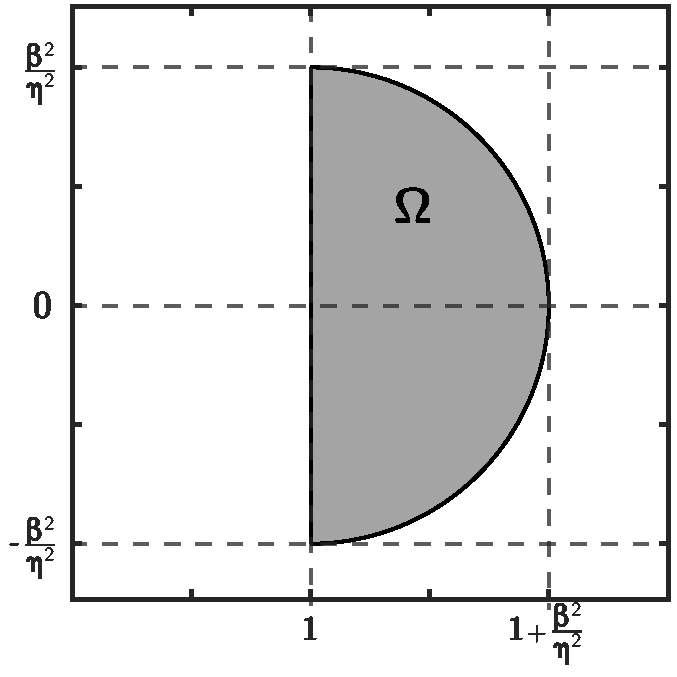
\includegraphics[width = 0.3\textwidth]{./fov_fig.pdf}
% \caption{}
% \label{fig:bound}
% \end{figure}
% %

% However, $\eta$ is probably not the best constant to use. For SPD matrices, 
% somebody proved that using a constant $k := \sqrt{\eta^2+\beta^2}$ and
% preconditioner
% %
% \begin{align*}
% P_k := (k I - \mathcal{L})^{-2}
% \end{align*}
% %
% is a much better choice for $\beta \gg \eta$. I am trying to figure out if
% anything similar can be said for the FOV (or other more general types of
% analysis/operator).

% Note that for real $k>0$, $W\left[\left(I - \tfrac{1}{k}\mathcal{L}\right)^{-1}\right]$ and
% $W\left[\left(I - \tfrac{1}{k}\mathcal{L}\right)^{-2}\right]$ are contained in
% the positive half unit circle. Now consider the more general preconditioning
% %
% \begin{align}\nonumber
% (kI - \mathcal{L})^{-2}\Big[(nI - \mathcal{L})^2 + \beta^2 I\Big] 
% 	& = (kI - \mathcal{L})^{-2}\Big[(\eta-k)I + (kI - \mathcal{L}))^2 + \beta^2 I\Big] \\
% & = (kI - \mathcal{L})^{-2}\Big[(k-\eta)^2I - 2(k-\eta)(kI - \mathcal{L}) + (kI - \mathcal{L})^2 + \beta^2 I\Big] \nonumber\\
% & = I - 2(k-\eta)(kI - \mathcal{L})^{-1} + (\beta^2 + (k-\eta)^2)(kI - \mathcal{L})^{-2} \nonumber\\
% & = I - 2\frac{k-\eta}{k}\left(I - \tfrac{1}{k}\mathcal{L}\right)^{-1} + \frac{\beta^2 + (k-\eta)^2}{k^2}
% 	\left(I - \tfrac{1}{k}\mathcal{L}\right)^{-2}.\label{eq:gen0}
% \end{align}
% %
% Note that we have a quadratic polynomial in $\left(I - \tfrac{1}{k}\mathcal{L}\right)^{-1}$.
% Let $\alpha$ denote the inverse of the roots of the corresponding polynomial.
% Then \eqref{eq:gen1} can be expressed in factored form as
% %
% \begin{align*}
% (kI - \mathcal{L})^{-2}\Big[(nI - \mathcal{L})^2 + \beta^2 I\Big] 
% 	& = \Big[I - \overline{\alpha}\left(I - \tfrac{1}{k}\mathcal{L}\right)^{-1}\Big]
% 	\Big[I - \alpha\left(I - \tfrac{1}{k}\mathcal{L}\right)^{-1}\Big],
% \end{align*}
% %
% where $\alpha + \overline{\alpha} = 2\tfrac{k-\eta}{k}$ and $\alpha\overline{\alpha}
% = \tfrac{\beta^2 + (k-\eta)^2}{k^2}$. For ease of notation, let us denote
% $\mathcal{P} := \left(I - \tfrac{1}{k}\mathcal{L}\right)^{-1}$.
% {\color{blue}
% We are now interested in the field of values of 
% %
% \begin{align*}
% \mathcal{Z} := (I - \overline{\alpha}\mathcal{P})(I - {\alpha}\mathcal{P}).
% \end{align*}
% %
% where $W(\mathcal{P})$ is contained in the positive half of the unit circle.
% This seems like a nice structure and operator, but I'm stuck. I've tried the
% standard symmetric and skew symmetric splittings. The symmetric works okay for
% an opper bound, but I cannot get a lower bound $> 0$. This is all related to
% \eqref{eq:gen0}, in particular how $\langle \mathcal{P}\mathbf{x},\mathbf{x}\rangle$
% and $\langle \mathcal{P}^2\mathbf{x},\mathbf{x}\rangle$ relate? In general I know
% the FOV of $A$ and $A^2$ don't necessarily relate, but there's a lot of nice
% structure here, and numerical results make $k = \sqrt{\eta^2+\beta^2}$ seem
% optimal for very nonsymmetric advective matrices as well.
% }


% % ------------------------------------------------------------------- %
% % ------------------------------ WRONG ------------------------------
% % ------------------------------------------------------------------- %
% \section{Old analysis different consatnts, SPD operators}

% \tcr{THIS IS WRONG BECAUSE CANNOT POSE AS QUADRATIC POLYNOMIAL WITH DIFFERENT CONSTANTS}

% Suppose $\widehat{\mathcal{L}}$ is symmetric negative definite and, thus, has an orthogonal
% basis of eigenvectors, and consider the conditioning of \eqref{eq:gamma0}. Assume that the
% eigenvalues of $( I- \tfrac{1}{\eta}\widehat{\mathcal{L}})^{-1} \subset (0,1)$, and are
% somewhat dense in this interval. This is to be expected for parabolic problems, where the
% eigenvalues of $-\widehat{\mathcal{L}}$ range from $\sim \delta t$ to $\sim \delta t/h^2$,
% which typically corresponds to $\sim(0,\infty)$ as $h,\delta t\to 0$.

% Note that \eqref{eq:gamma0} is a quadratic polynomial in an SPD operator, and the
% eigenvalues of \eqref{eq:gamma0} are then a quadratic function $P(\lambda)$ of the
% eigenvalues $\{\lambda\}$ of $\widehat{\mathcal{L}}$, where
% %
% \begin{align}\label{eq:quadratic}
% P(\lambda,\gamma) &:= \frac{\beta^2}{\gamma\eta}\lambda^2 - \frac{\gamma - \eta}{\gamma}\lambda + 1.
% \end{align}
% %
% Assume that we choose $\gamma$ such that \eqref{eq:gamma0} is also SPD (choosing otherwise
% would be a poor choice in terms of conditioning). Then the condition number of
% \eqref{eq:gamma0} is given by
% %
% \begin{align}\label{eq:cond0}
% \textnormal{cond}\left((\gamma I- \widehat{\mathcal{L}})^{-1}S\right) & =
% 	\frac{\lambda_{\max}\left((\gamma I- \widehat{\mathcal{L}})^{-1}S\right)}
% 		{\lambda_{\min}\left((\gamma I- \widehat{\mathcal{L}})^{-1}S\right)}.
% \end{align}
% %
% Again assuming that eigenvalues $\lambda\in\sigma\left(\widehat{\mathcal{L}}\right)$ take
% on values $\lambda\in(0,1)$, the condition number \eqref{eq:cond0} can be expressed
% precisely as $h,\delta t\to 0$ via
% %
% \begin{align}\label{eq:cond1}
% \textnormal{cond}\left((\gamma I- \widehat{\mathcal{L}})^{-1}S\right) & =
% 	\frac{\max_{x\in(0,1)} P(x,\gamma)}{\min_{y\in(0,1)} P(y,\gamma)}.
% \end{align}
% %
% With this closed form, it is natural to pose a minimization problem to find the
% optimal $\gamma$ in terms of minimizing the condition number \eqref{eq:cond0}.
% We make the assumption that $\eta \leq \gamma \leq \eta^2+\beta^2$, and consider
% the problem
% %
% \begin{align*}
% \gamma_* & = \textnormal{argmin}_{\gamma \geq \eta}
% 	\frac{\max_{x\in(0,1)} P(x,\gamma)}{\min_{y\in(0,1)} P(y,\gamma)}.
% \end{align*}
% %

% For $\gamma > 0$, $P(\lambda,\gamma)$ is concave up in $\lambda$, and thus
% the maximum over a closed interval $[0,1]$ will be obtained at one of the
% end points,
% %
% \begin{align*}
% P(0) = 1, \hspace{5ex} P(1) = \frac{\eta^2+\beta^2}{\eta\gamma}.
% \end{align*}
% %
% For the maximum eigenvalue, this yields
% %
% \begin{align}\label{eq:max0}
% \lambda_{\max} & = \begin{cases} 
% 	\frac{\eta^2+\beta^2}{\gamma\eta} & \gamma\leq \frac{\eta^2+\beta^2}{\eta}, \\
% 	1 & \gamma > \frac{\eta^2+\beta^2}{\eta}.
% 	\end{cases}
% \end{align}
% %
% If there is a critical point within the interval $(0,1)$, the minimum
% will be obtained at this critical point, otherwise it will be obtained
% at the other endpoint (i.e., not where the maximum is obtained). Solving
% for $\tfrac{\partial P(\lambda,\gamma)}{\lambda}$ and setting equal to
% zero, we have a root
% %
% \begin{align*}
% \lambda_0 := \frac{\eta(\gamma-\eta)}{ 2\beta^2} \geq 0, \hspace{5ex}
% P(\lambda_0,\gamma) & = 1 - \frac{\eta(\gamma-\eta)^2}{4\beta^2\gamma},
% \end{align*}
% %
% which satisfies $\lambda_0<1$ when $\gamma < \tfrac{2\beta^2+\eta^2}{\eta}$.
% If we suppose $\lambda_0<1$, we have 
% %
% \begin{align}\label{eq:min0}
% \lambda_{\min} & = P(\lambda_0,\gamma) = 1 - \frac{\eta(\gamma-\eta)^2}{4\beta^2\gamma}.
% \end{align}
% %
% For $\gamma \geq \tfrac{\eta^2+2\beta^2}{\eta} > \tfrac{\eta^2+\beta^2}{\eta}$,
% from \eqref{eq:max0}, we have $\lambda_{\min} = \frac{\eta^2+\beta^2}{\gamma\eta}$.
% Altogether, we have the condition number as a continuous function of $\gamma$,
% %
% \begin{align}\label{eq:cases}
% \textnormal{cond}\left((\gamma I- \widehat{\mathcal{L}})^{-1}S\right) & =
% % 	\begin{cases}
% % 		\frac{\frac{\eta^2+\beta^2}{\gamma\eta}}{1 - \frac{\eta(\gamma-\eta)^2}{4\beta^2\gamma}}
% % 			& \gamma\leq \frac{\eta^2+\beta^2}{\eta}, \\
% % 		\frac{1}{1 - \frac{\eta(\gamma-\eta)^2}{4\beta^2\gamma}}
% % 			& \frac{\eta^2+\beta^2}{\eta} \leq \gamma\leq \frac{\eta^2+2\beta^2}{\eta}, \\
% % 		\frac{1}{\frac{\eta^2+\beta^2}{\gamma\eta}}
% % 			& \frac{\eta^2+2\beta^2}{\eta} \leq \gamma.
% % 	\end{cases}
% % \\ & = \textnormal{argmin}_{\gamma \in[\eta,\eta^2+\beta^2]} 
% 	\begin{cases}
% 		\frac{4\beta^2(\eta^2+\beta^2)}{4\beta^2\gamma\eta - \eta^2(\gamma-\eta)^2}
% 			& \eta \leq \gamma< \frac{\eta^2+\beta^2}{\eta}, \\
% 		\frac{4\beta^2\gamma}{4\beta^2\gamma - \eta(\gamma-\eta)^2}
% 			& \frac{\eta^2+\beta^2}{\eta} \leq \gamma < \frac{\eta^2+2\beta^2}{\eta}, \\
% 		\frac{\gamma\eta}{\eta^2+\beta^2}
% 			& \frac{\eta^2+2\beta^2}{\eta} \leq \gamma.
% 	\end{cases}
% \end{align}
% %
% To proceed with the proof, we consider each of these cases individually.\\
% \\
% \underline{$\mathbf{\frac{\boldsymbol{\eta}^2+2\boldsymbol{\beta}^2}{\boldsymbol{\eta}}
% 	\leq \boldsymbol{\gamma}:}$}
% This is the simplest case. Simply note that for $0<\eta\leq \gamma$,
% %
% \begin{align*}
% \frac{\partial}{\partial\gamma} \left[\frac{\gamma\eta}{\eta^2+\beta^2}\right] = 
% 	\frac{\eta}{\eta^2+\beta^2} > 0,
% \end{align*}
% %
% and thus the minimum value for $\gamma \geq \frac{\eta^2+2\beta^2}{\eta}$ is
% obtained at the lower point of the interval, $\gamma = \frac{\eta^2+2\beta^2}{\eta}$.\\
% \\
% \underline{$\mathbf{\frac{\boldsymbol{\eta}^2+\boldsymbol{\beta}^2}{\boldsymbol{\eta}} \leq
% 	\boldsymbol{\gamma} < \frac{\boldsymbol{\eta}^2+2\boldsymbol{\beta}^2}{\boldsymbol{\eta}}}$:}
% Taking the derivative with respect to $\gamma$ from the appropriate equation in
% \eqref{eq:cases}, we get nice cancellation to arrive at
% %
% \begin{align*}
% \frac{\partial}{\partial\gamma} \left[\frac{4\beta^2\gamma}{4\beta^2\gamma - \eta(\gamma-\eta)^2}\right] 
% 	& = 4\beta^2\eta \frac{\gamma^2 - \eta^2}{\left(4\beta^2\gamma - \eta(\gamma-\eta)^2\right)^2}
% 	> 0.
% \end{align*}
% %
% As in the previous case, this yields the minimum value for $\gamma \in\left[\tfrac{\eta^2+\beta^2}{\eta} ,
% \tfrac{\eta^2+2\beta^2}{\eta}\right]$ is obtained at the lower point of the interval,
% $\gamma = \frac{\eta^2+\beta^2}{\eta}$.\\
% \\
% \underline{$\mathbf{\boldsymbol{\eta} \leq \boldsymbol{\gamma}} <
% 	\frac{\boldsymbol{\eta}^2+\boldsymbol{\beta}^2}{\boldsymbol{\eta}}:$}
% Again taking the derivative with respect to $\gamma$ yields
% %
% \begin{align}\label{eq:deriv_gam}
% \frac{\partial}{\partial\gamma} \left[\frac{4\beta^2(\eta^2+\beta^2)}{4\beta^2\gamma\eta
% 	- \eta^2(\gamma-\eta)^2}\right] & =
% 	\frac{4\beta^2(\eta^2+\beta^2)}{\left(4\beta^2\gamma\eta - \eta^2(\gamma-\eta)^2\right)^2}
% 	\left(2\eta^2\gamma - 4\beta^2\eta - 2\eta^3 \right).
% \end{align}
% %
% Note that the sign (and root) of \eqref{eq:deriv_gam} is fully determined by 
% the term on the right, $(2\eta^2\gamma - 4\beta^2\eta - 2\eta^3 )$.
% Setting equal to zero and solving, we have a root at
% %
% \begin{align*}
% \gamma_0 := \frac{2\beta^2 + \eta^2}{\eta} > \frac{\beta^2+\eta^2}{\eta},
% \end{align*}
% %
% where \eqref{eq:deriv_gam} is $<0$ for $\gamma < \gamma_0$. Thus,
% \eqref{eq:deriv_gam} is $<0$ for all $\gamma \in[\eta,\tfrac{\eta^2+\beta^2}{\eta}]$,
% and the minimum value of the function is obtained at the upper end of the interval,
% $\gamma = \frac{\eta^2+\beta^2}{\eta}$.

% Combining the above cases, we have
% %
% \begin{align}\label{eq:gamma_opt}
% \gamma_* & := \frac{\eta^2+\beta^2}{\eta}.
% \end{align}
% %
% with condition number
% %
% \begin{align}\label{eq:opt_cond}
% \textnormal{cond}\left((\gamma_* I- \widehat{\mathcal{L}})^{-1}S\right) & =
% 	1 + \frac{\beta^2}{3\beta^2 + 4\eta^2},
% \end{align}
% %
% whereas using $\eta$ instead of $\gamma_*$ yields condition number
% $1 + \tfrac{\beta^2}{\eta^2}$ \eqref{eq:cases}. Interestingly, if we look at
% the product of the two constants, $\eta\gamma_* = \eta^2+\beta^2$, we have
% the same as when we use a single constant twice in \eqref{eq:gamma_opt0},
% $\gamma_\times^2 = (\sqrt{\eta^2+\beta^2})^2 = \eta^2+\beta^2$.





% ---------------------------------------------------------------------------------------------- %
% --------------------- Incorrect eigenvalue analysis
% ---------------------------------------------------------------------------------------------- %
% \subsubsection{Remainder of Ben's analysis}
% In choosing $\gamma$, note that $\mathcal{F}(\gamma,\lambda_-) < 0$, which contradicts
% the assumption of positive definiteness. Thus, we must make an additional assumption
% that $\lambda_-\not\in(0,\infty)$.\footnote{\tcb{OAK: But why \textit{must} we assume that $\mathcal{F}(\gamma,\lambda_-) < 0$ implies/requires/means that $\lambda_- < 0$?}} From \eqref{eq:roots}, this is equivalent to saying that
% %
% \begin{align*}
% \beta^2-\eta(\gamma-\eta) & < \beta\sqrt{\beta^2+(\gamma-\eta)^2}, \\
% \Longleftrightarrow\hspace{19.5ex}
% \left(\beta^2-\eta(\gamma-\eta)\right)^2& < \beta^2\left(\beta^2+(\gamma-\eta)^2\right), \\
% \Longleftrightarrow\hspace{5ex}
% (\gamma-\eta)\left[\beta^2(\gamma+\eta) - \eta^2(\gamma-\eta)\right] & > 0, \\
% \Longleftrightarrow\hspace{24ex}
% \frac{\beta^2}{\eta^2} > \frac{\gamma-\eta}{\gamma+\eta}.
% \end{align*}
% %
% Noting that $\tfrac{\gamma-\eta}{\gamma+\eta} < 1$, the above constraint clearly holds
% for $\beta > \eta$, which is the only regime in which we need a better constant anyways.

% Assume now that $\beta > \eta$, in which case maxima and minima of
% $\mathcal{F}(\gamma,\lambda)$ in $\lambda$ can be obtained at
% $\lambda\in\{0,\lambda_+,\infty\}$. Note for $\gamma < \sqrt{\eta^2+\beta^2}$,
% %
% \begin{align*}
% \max_{\lambda\in[0,\infty)} \mathcal{F}(\gamma,\lambda) & =
% 	1 + \frac{\eta^2+\beta^2 - \gamma^2}{\eta\gamma} > 1, \\
% \min_{\lambda\in[0,\infty)} \mathcal{F}(\gamma,\lambda) & =
% 	\frac{2\beta}{\beta + \sqrt{\beta^2 + (\gamma-\eta)^2}} < 1,
% \end{align*}
% %
% while for $\gamma \geq \sqrt{\eta^2+\beta^2}$,
% %
% \begin{align*}
% \max_{\lambda\in[0,\infty)} \mathcal{F}(\gamma,\lambda) & = 1, \\
% \min_{\lambda\in[0,\infty)} \mathcal{F}(\gamma,\lambda) & =
% 	\min\left\{\mathcal{F}(\gamma,0),\mathcal{F}(\gamma,\lambda_+)\right\}.
% \end{align*}
% %

% Returning to \eqref{eq:gam_opt}, let us start with the case
% $\gamma \geq \sqrt{\eta^2+\beta^2}$. We will do show by showing that both
% $\tfrac{1}{\mathcal{F}(\gamma,0)}$ and $\tfrac{1}{\mathcal{F}(\gamma,\lambda_+)}$
% are minimized over $\gamma \geq \sqrt{\eta^2+\beta^2}$ at
% $\gamma = \sqrt{\eta^2+\beta^2}$ (because the maximum eigenvalue is 1).
% For $\mathcal{F}(\gamma,\lambda_+)$, taking the partial of
% $\tfrac{1}{\mathcal{F}(\gamma,\lambda_+)}$ with respect to $\gamma$ yields
% %
% \begin{align*}
% \frac{\gamma-\eta}{2\beta\sqrt{\beta^2+(\gamma-\eta)^2}} > 0,
% \end{align*}
% %
% which implies the minimum is obtained at the beginning of the interval, in
% this case $\gamma = \sqrt{\eta^2+\beta^2}$. Analogous derivations hold when
% evaluating at $\lambda=0$, yielding the optimal $\gamma \geq \sqrt{\eta^2+\beta^2}$
% with respect to \eqref{eq:gam_opt} given by $\gamma = \sqrt{\eta^2+\beta^2}$.

% For $\gamma < \sqrt{\eta^2+\beta^2}$, we will also consider the derivative
% of \eqref{eq:gam_opt} in $\gamma$ to minimize, but without explicit construction.
% Consider $\gamma_*$ as a product rule of $\lambda_{\max}(\gamma)\cdot
% \lambda_{\min}(\gamma)$, where
% %
% \begin{align*}
% \lambda_{\max}(\gamma) := 1 + \frac{\eta^2+\beta^2 - \gamma^2}{\eta\gamma}, \hspace{5ex}
% \lambda_{\min}(\gamma) := \frac{\beta + \sqrt{\beta^2 + (\gamma-\eta)^2}}{2\beta}.
% \end{align*}
% %
% It is straightforward to verify that for all $\gamma\in(\eta,\sqrt{\eta^2+\beta^2})$,
% $\lambda_{\max}(\gamma) > 0$, $\lambda_{\min}(\gamma) > 0$, $\lambda_{\min}'(\gamma) > 0$,
% and $\lambda_{\max}'(\gamma) < 0$. The derivative of \eqref{eq:gam_opt} is then
% given by 
% %
% \begin{align*}
% \mathcal{D}(\gamma) := \lambda_{\max}(\gamma)\lambda_{\min}'(\gamma) +
% 	\lambda_{\max}'(\gamma)\lambda_{\min}(\gamma),
% \end{align*}
% %
% and to show $\mathcal{D}(\gamma) < 0$ for $\gamma\in(\eta,\sqrt{\eta^2+\beta^2})$,
% it is sufficient to show that
% %
% \begin{equation*}
% -\lambda_{\max}'(\gamma)\lambda_{\min}(\gamma) > \lambda_{\max}(\gamma)\lambda_{\min}'(\gamma).
% \end{equation*}
% %
% Plugging in, we want to show
% %
% \begin{align*}
% \left(\frac{1}{\eta} + \frac{\eta^2+\beta^2}{\eta\gamma^2}\right)
% 	\left(\frac{\beta + \sqrt{\beta^2 + (\gamma-\eta)^2}}{2\beta}\right) 
% & > \left(\frac{\gamma-\eta}{2\beta\sqrt{\beta^2+(\gamma-\eta)^2}} \right)
% 	\left(\frac{\eta\gamma+\eta^2+\beta^2-\gamma^2}{\eta\gamma}\right), \\
% \left(\eta^2+\beta^2+\gamma^2\right)
% 	\left(\beta^2 + (\gamma-\eta)^2 + \beta\sqrt{\beta^2+(\gamma-\eta)^2}\right)
% & > \gamma(\gamma-\eta)\left(\eta\gamma+\eta^2+\beta^2-\gamma^2\right).
% \end{align*}
% %
% Then note that for the first term on each side,
% %
% \begin{align*}
% 2\gamma(\gamma-\eta) = 2\gamma^2 - 2\gamma\eta < 2\gamma^2 \leq \eta^2+\beta^2 + \gamma^2.
% \end{align*}
% %
% For the second, first note that $\beta\sqrt{\beta^2+(\gamma-\eta)^2} < \beta^2$.
% Then we want to show that
% %
% \begin{align*}
% 2\beta^2 + (\gamma-\eta)^2 & > \frac{1}{2}\left(\eta\gamma+\eta^2+\beta^2-\gamma^2\right), \\
% 4\beta^2 + 2\gamma^2 + 2\eta^2 - 4\gamma\eta & > \eta\gamma+\eta^2+\beta^2-\gamma^2, \\
% 3\beta^2 + 3\gamma^2 + \eta^2 & > 5 \gamma\eta.
% \end{align*}
% %
% Noting that $5\gamma\eta < 5\gamma^2$, it is sufficient to show that 
% %
% \begin{align*}
% 3\beta^2 + 3\gamma^2 + \eta^2 & > 5 \gamma^2, \\
% 3\beta^2 + \eta^2 & > 2 \gamma^2.
% \end{align*}
% %
% Finally, by assumption that $\gamma < \sqrt{\eta^2+\beta^2}$ and $\beta > \eta$,
% we have $2\gamma^2 < 2\eta^2+2\beta^2 < 3\beta^2+\eta^2$.

% Altogether, we have that for $\gamma \in(\eta,\sqrt{\eta^2+\beta^2})$,
% %
% \begin{align*}
% \frac{\partial}{\partial\gamma}\left[ 
% 	\frac{\max_{\lambda\in[0,\infty)} \mathcal{F}(\gamma,\lambda)}
% 	{\min_{\lambda\in[0,\infty)} \mathcal{F}(\gamma,\lambda)} \right] < 0
% \end{align*}
% %
% meaning the optimal $\gamma \in(\eta,\sqrt{\eta^2+\beta^2})$ with respect to
% \eqref{eq:gam_opt} is given by the maximum $\gamma = \sqrt{\eta^2+\beta^2}$.
% Plugging in, we can evaluate our resulting bound as
% %
% \begin{align}\label{eq:cond_opt}
% \textnormal{cond}\left((\gamma_* I- \widehat{\mathcal{L}})^{-1}S\right) & =
% 	\frac{1}{2} + \frac{\sqrt{(\eta^2+\beta^2) - \eta\sqrt{\eta^2+\beta^2}}}{\sqrt{2}\beta}.
% \end{align}
% %
% \tcb{This seems to small, need to check closer/make sure algebra is correct
% and the resulting condition numbers are reasonable.}